\documentclass[11pt,oneside]{article}    %use"amsart"insteadof"article"forAMSLaTeXformat
\usepackage{geometry}        %Seegeometry.pdftolearnthelayoutoptions.Therearelots.
\geometry{letterpaper}        %...ora4paperora5paperor...
%\geometry{landscape}        %Activateforforrotatedpagegeometry
%\usepackage[parfill]{parskip}        %Activatetobeginparagraphswithanemptylineratherthananindent
\usepackage{graphicx}                %Usepdf,png,jpg,orepsßwithpdflatex;useepsinDVImode
                                %TeXwillautomaticallyconverteps-->pdfinpdflatex        
\usepackage{amssymb}
\usepackage[colorlinks]{hyperref}

%----macros begin---------------------------------------------------------------
\usepackage{color}
\usepackage{amsthm}

\def\conv{\mbox{\textrm{conv}\,}}
\def\aff{\mbox{\textrm{aff}\,}}
\def\I{\mathbb{I}}
\def\E{\mathbb{E}}
\def\R{\mathbb{R}}
\def\Z{\mathbb{Z}}
\def\tex{\TeX}
\def\latex{\LaTeX}
\def\v#1{{\bf #1}}
\def\p#1{{\bf #1}}
\def\T#1{{\bf #1}}

\def\vet#1{{\left(\begin{array}{cccccccccccccccccccc}#1\end{array}\right)}}
\def\mat#1{{\left(\begin{array}{cccccccccccccccccccc}#1\end{array}\right)}}

\def\lin{\mbox{\rm lin}\,}
\def\aff{\mbox{\rm aff}\,}
\def\pos{\mbox{\rm pos}\,}
\def\cone{\mbox{\rm cone}\,}
\def\conv{\mbox{\rm conv}\,}
\newcommand{\homog}[0]{\mbox{\rm homog}\,}
\newcommand{\relint}[0]{\mbox{\rm relint}\,}

%----macros end-----------------------------------------------------------------

\title{Concept and preliminary design of a hospital system
\footnote{This document is part of the \emph{Linear Algebraic Representation with CoChains} (LAR-CC) framework~\cite{cclar-proj:2013:00}. \today}
}
\author{Alberto Paoluzzi}
%\date{}                            %Activatetodisplayagivendateornodate

\begin{document}
\maketitle
\nonstopmode
\tableofcontents

\begin{abstract}
In this module we develop stepwise the concept and the preliminary building program of a hospital of medium size, using as source the document~\cite{who:2013} of the World Health Organisation. The main aim of this modelling is to make experiments with ``cochain calculus'' over a cell decomposition of a quite complex engineering project. It may be useful to exemplify some characters of a model-based engineering approach to the initial, and more important setps of an engineering project.
\end{abstract}

\section{Introduction}

The development of the geometric model of a general hospital, and some computational experiments of model-based engineering, is the topic and the main aim of this software module.

\section{Model planning}

\subsection{Data sources}

The starting point of the modelling developed here is the paper~\cite{who:2013}, about Hospital Planning and Design, downloadable from~\href{http://paoluzzi.dia.uniroma3.it/web/hospital-planning-and-design.pdf}{here}, and in particular the two images shown in Figure~\ref{fig:hismail} and relative to the functional zoning of floors, and providing an axonometric view of the vertical organisation of the hospital.

\begin{figure}[htbp] %  figure placement: here, top, bottom, or page
   \centering
   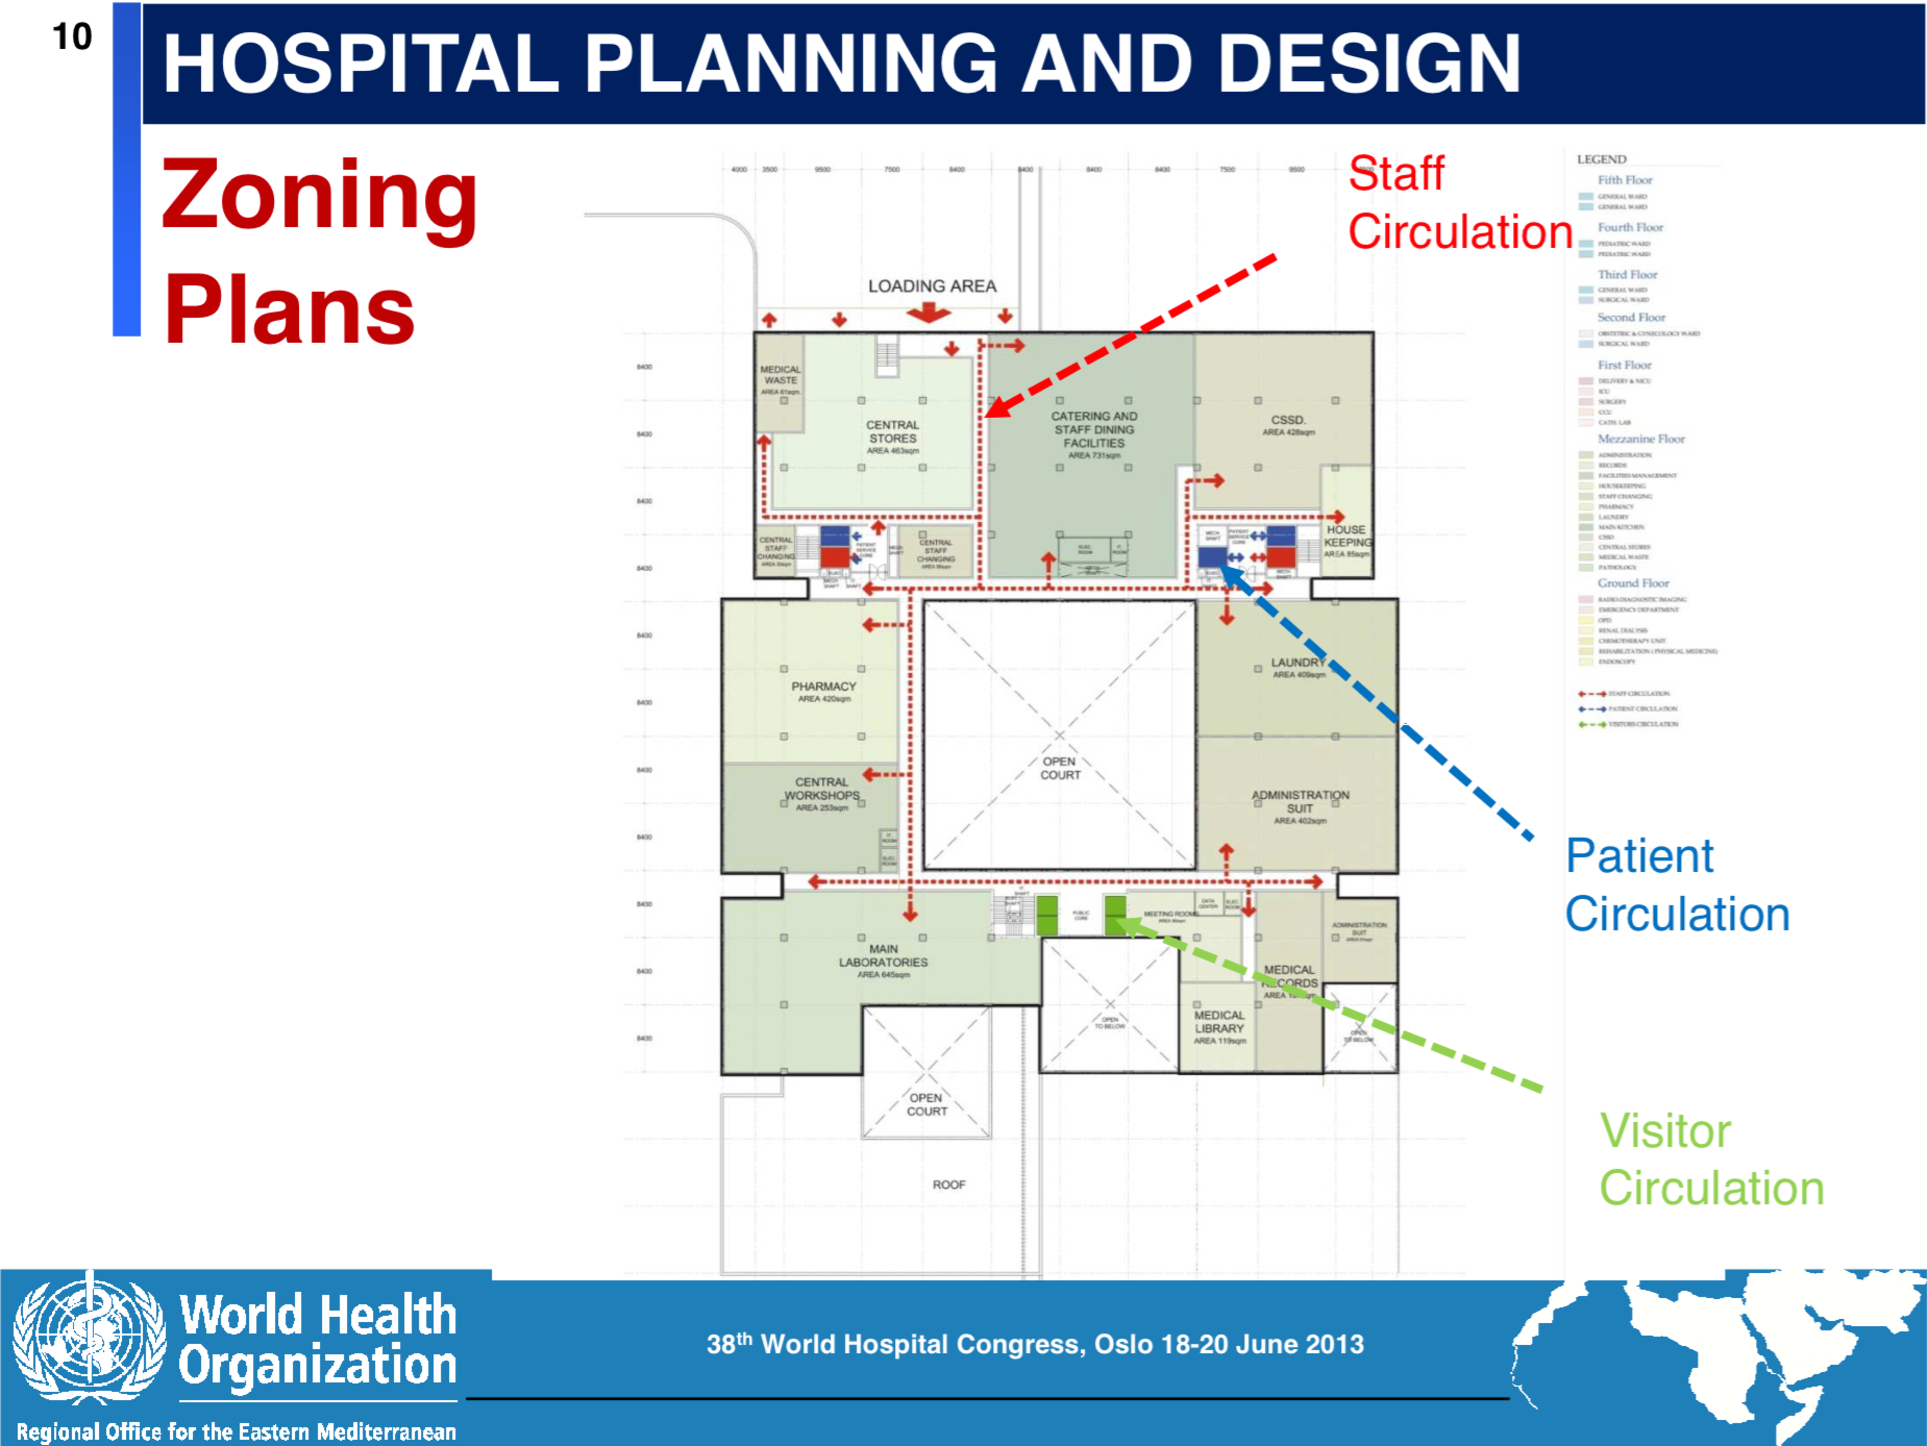
\includegraphics[width=0.495\linewidth]{images/hismail-1} 
   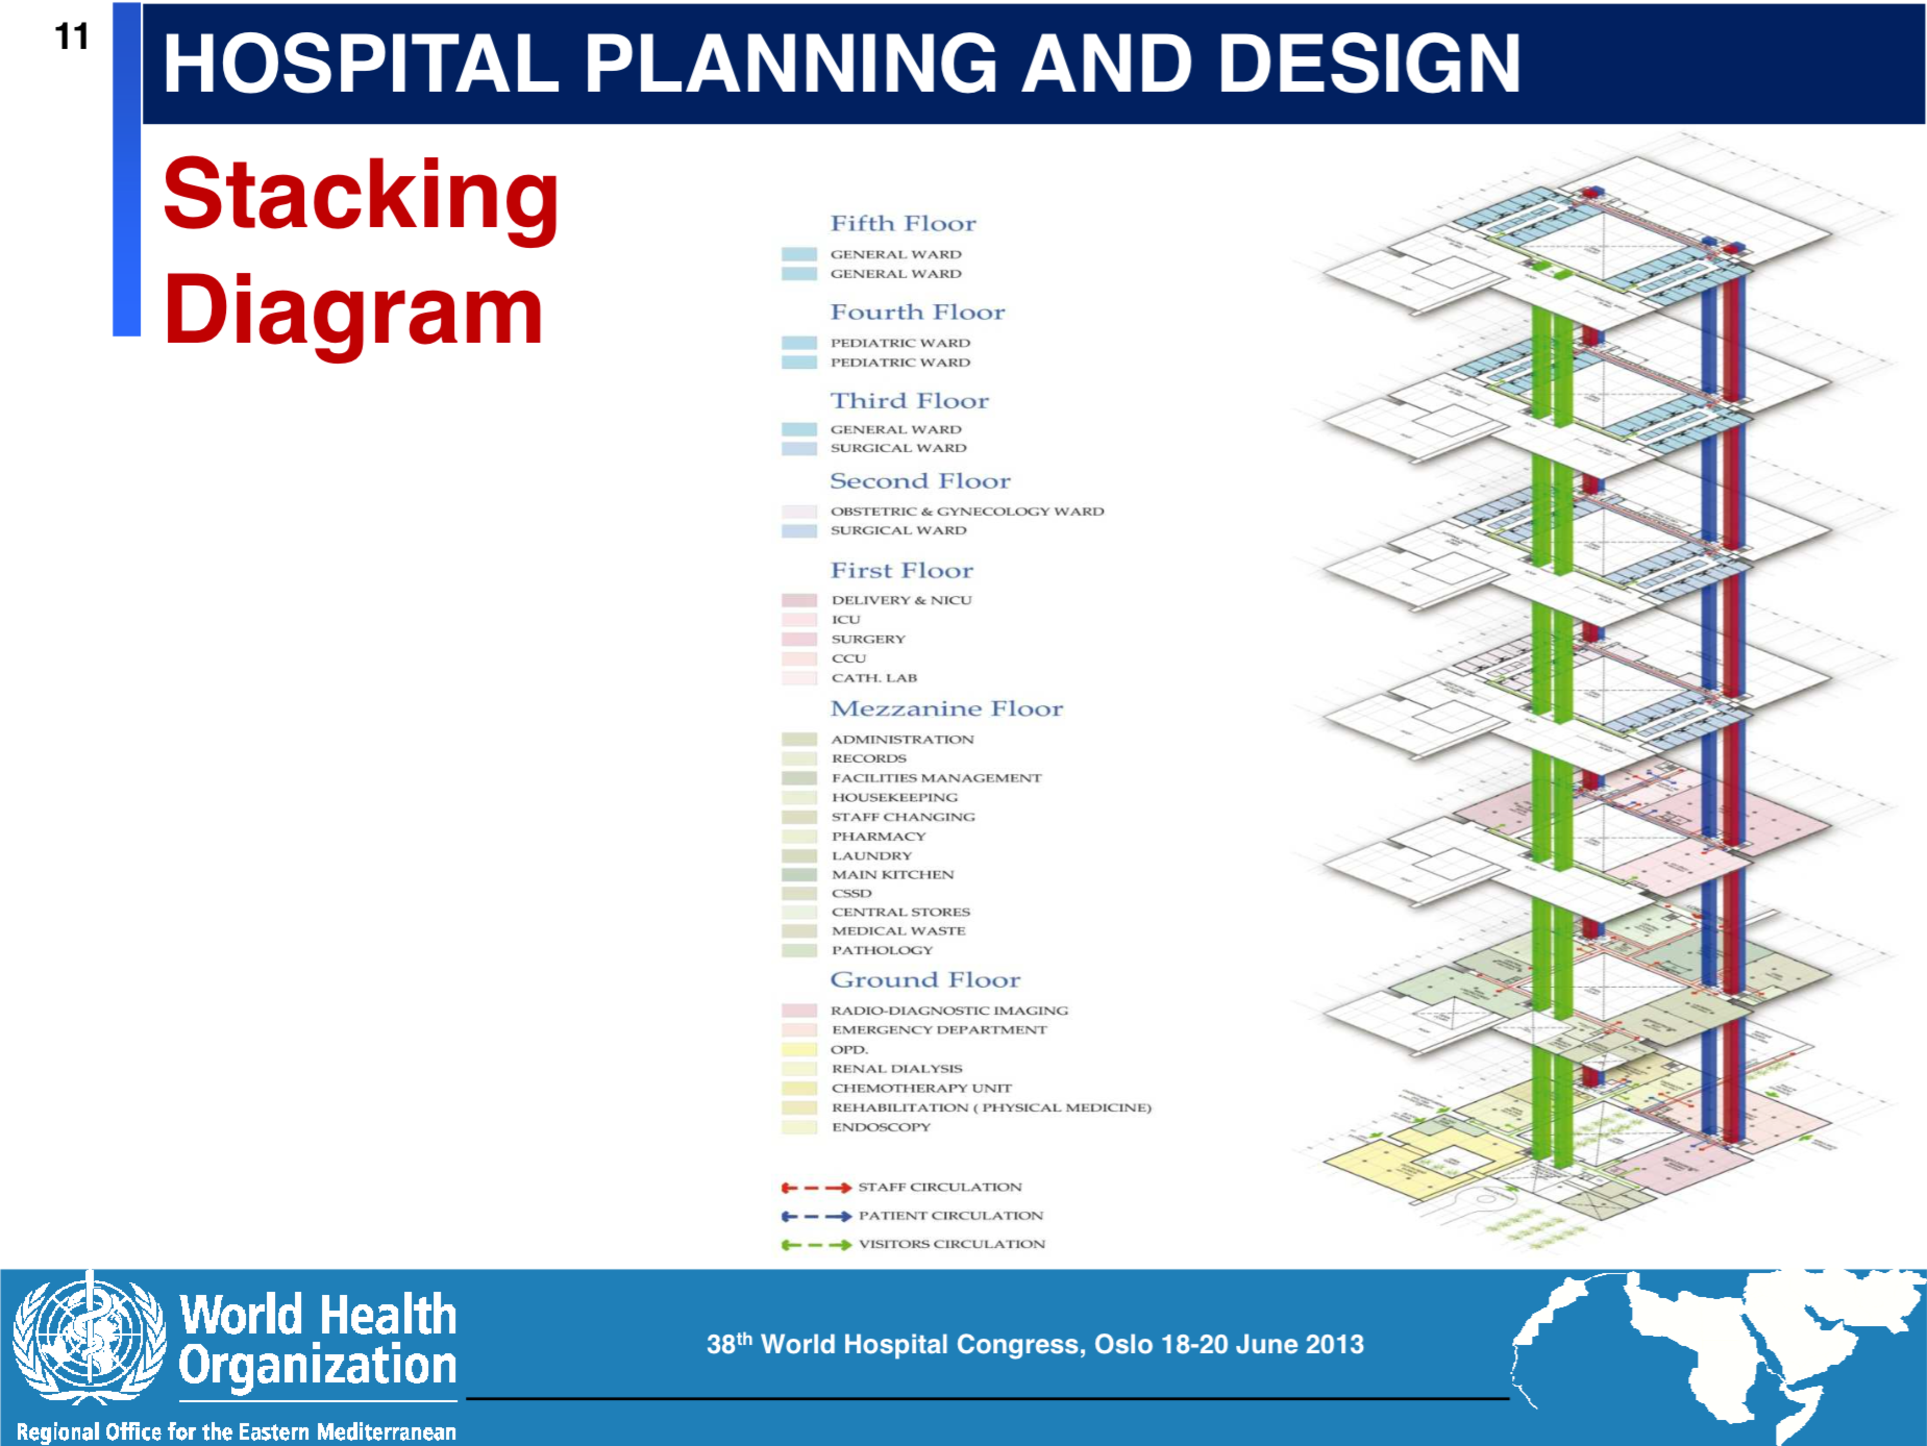
\includegraphics[width=0.495\linewidth]{images/hismail-2} 
   \caption{Two images of the example model for hospital planning and design used in this module: (a) functional zoning of the mezzanine floor; (b) axonometric view of the vertical design organisation.}
   \label{fig:hismail}
\end{figure}

\subsection{Reference grid}
\label{sec:grid}

Looking at the images of Figure~\ref{fig:hismail}, it is easy to notice the presence of a very regular structural frame, providing in the following a reference grid for the numeric input of the geometry of the departments and floors of the hospital model. Some images with evidenced (in blue) the structural frame grid are shown in Figure~\ref{fig:referencegrid}.

It may be useful to underline that the grid step in the $y$ direction (from top to bottom of the drawings) is constant and equal to $8.4 m$, whereas the grid in the $x$ direction (from left to right of the drawings) alternates the $[7.5,9.5,7.5] m$ pattern with the step-size used in the other direction ($8.4 m$).  the above numeric patterns are actually derived by the architect from the layout of the inpatient wards.

Notice also that both grid directions, and of course the structural frame of the building, are aligned with the \emph{inpatient wards}, that supply one the main ideas of the design concept as a whole.


\begin{figure}[htbp] %  figure placement: here, top, bottom, or page
   \centering
   \includegraphics[width=0.495\linewidth]{images/firstfloor} 
   \includegraphics[width=0.495\linewidth]{images/secondfloor} 
   \caption{The zooming of two floor plans, with evidentced the structural grid (in blue): (a) first floor; (b) second floor.}
   \label{fig:referencegrid1}
\end{figure}

\paragraph{Reference grid}

The reference grid is defined as \texttt{structuralGrid} in the script below, where \texttt{PROD} is the \texttt{pyplasm} primitive for Cartesian product of geometric values. The global variable \texttt{YMAX} is used in this module to compute (in the \texttt{metric} function) a proper coordinate transformation of the model from the reference frame used in the 2D hospital drawings (origin at top-left point, $y$ pointing downwards---see Figure~\ref{fig:referencegrid1}) to the standard righthand reference frame (origin at bottom-left point, $y$ pointing upwards---see Figure~\ref{fig:referencegrid2}).

%-------------------------------------------------------------------------------
@D Reference grid
@{""" Reference grid """
X = [0]+[7.5,9.5,7.5]+4*[8.4]+[7.5,9.5,7.5]+[0]
Y = [0]+14*[8.4]+[0]
xgrid = QUOTE(X[1:-1])
ygrid = QUOTE(Y[1:-1])
structuralGrid = PROD([xgrid,ygrid])
YMAX = SUM(Y)
@}
%-------------------------------------------------------------------------------


\begin{figure}[htbp] %  figure placement: here, top, bottom, or page
   \centering
   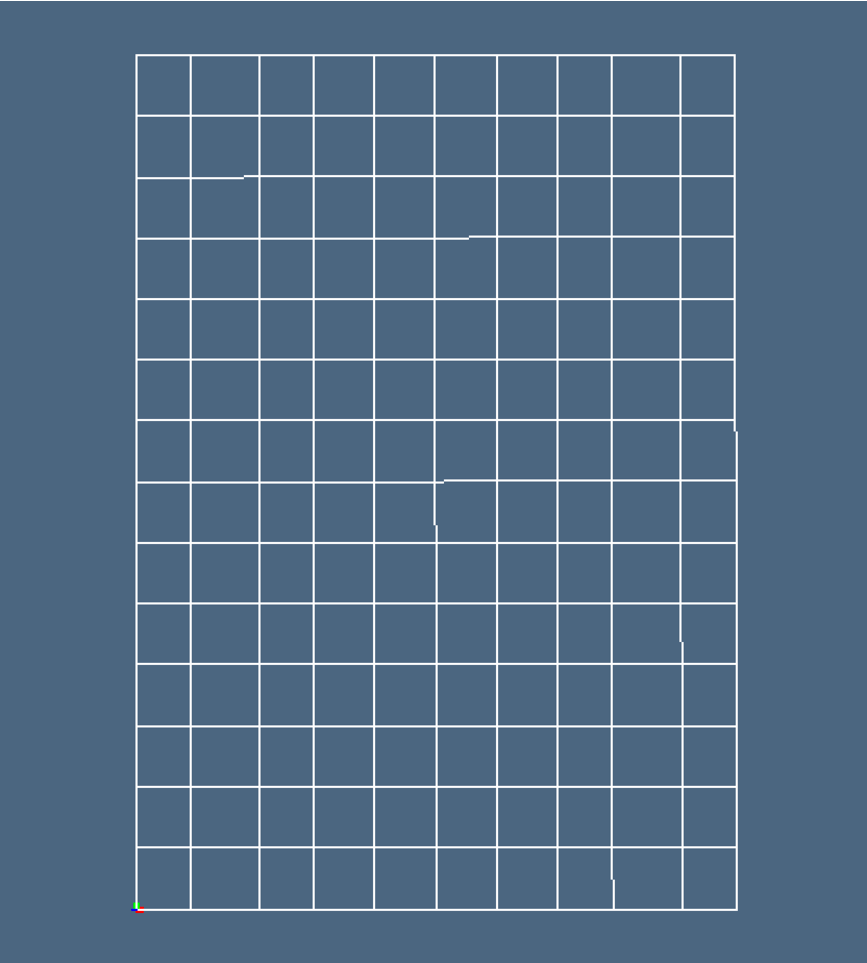
\includegraphics[width=0.33\linewidth]{images/hospitalgrid} 
   \caption{The reference grid used in the model construction. The intersections of grid lines have integer coordinates.}
   \label{fig:referencegrid2}
\end{figure}


\paragraph{From array indices to grid coordinates}

The reference grid, as the Cartesian product of two subsets of adjacent integers, will be used both to strongly simplify the input of data, and to assign to such coordinate numbers a more interesting meaning. For example the open space in the middle of the building will so defined as the 2D box with extreme points of integer coordinates $(3,4)$ and $(7,11)$.
Therefore the whole building  will be contained in the 2D interval $[0,10]\times [0,14]$ in ``\emph{grid coordinates}''.

%-------------------------------------------------------------------------------
@D From array indices to grid coordinates
@{""" From array indices to grid coordinates """
def index2coords(theArray):
    return CONS(AA(T([1,2]))(CAT((theArray).tolist())))
@}
%-------------------------------------------------------------------------------


\paragraph{From grid to metric coordinates}
The actual transformation of vertices of geometric data is executed by applying the (partial) function \texttt{metric} to a list of 2D points, as shown by the example below.

%-------------------------------------------------------------------------------
@D From grid to metric coordinates
@{""" From grid to metric coordinates """
def grid2coords(X,Y):
    xMeasures = list(cumsum(X))
    yMeasures = list(cumsum(Y))
    def grid2coords0(point):
        x,y = point[0:2]
        xint,yint = int(x), int(y)
        xdec,ydec = float(x-xint), float(y-yint)
        xcoord = xMeasures[xint] + xdec*X[xint+1]
        ycoord = yMeasures[yint] + ydec*Y[yint+1]
        if len(point)==2: return [xcoord, ycoord]
        else: return [xcoord, ycoord, point[2]]
    return grid2coords0

def coordMaps(YMAX):
    def coordMaps0(polyline):
        print "\npolyline =",polyline
        polyline = AA(grid2coords(X,Y))(polyline)
        polyline = vmap(YMAX)(polyline)
        return [eval(vcode(point)) for point in polyline]
    return coordMaps0

metric = coordMaps(YMAX)
@}
%-------------------------------------------------------------------------------


\paragraph{Example} 
A simple example of transformation from grid to metric coordinates is given here:
{\small 
\begin{verbatim}
polyline = metric([[3,4],[3,8],[4,8],[4,7.8],[6,7.8],[6,8],[6.65,8],[6.65,4]])
>>> [[24.5,84.0],[24.5,50.4],[32.9,50.4],[32.9,52.08],[49.7,52.08],[49.7,50.4],
     [55.16,50.4],[55.16,84.0]]
\end{verbatim}}



\subsection{Architecture of modeling process}

A short summary of the  modelling process of the whole hospital follows. First we found the schematic plans of the building,
and provided them with a reference grid by locating the main design choices about the structural frame.
Then we enter floor-wise the 2D geometry of the single storeys, as aggregations of hospital departments and services.
The input of data is made carefully, in order to get a snap of coincident vertices of adjacent departments, i.e.~of departments sharing some common edges. The input of geometry is done in grid coordinates, giving the boundary sequences of vertices in counterclockwise order. These are then transformed in LAR (Linear Algebraic Representation) data structures~\cite{Dicarlo:2014:TNL:2543138.2543294} and embedded into instances of the \texttt{Struct}, the \texttt{lar-cc} class for  hierarchical structures, in order to append some specific information (like the structure name, the containment box, and so on). At the end of this step the whole building is defined as the \texttt{Struct} made by his storeys. An embedding in 3D of such 2D geometric data provided a 2.5-dimensional mock-up of the building.


%===============================================================================
\section{Building units planning}
%===============================================================================

\subsection{Wire-frame input}

As already said, the data input for this project was made by hand. Of course, an
interactive user-interface in underway. I would like to notice that to enter apart the 
coordinates of the vertices of cells, as two (or three) adjacent arrays, is much 
faster and lesser in danger of getting errors than to enter an array of points as 
pairs of coordinates.

The several building units contained in this storey are given in the below script,
each associated to a single ordered polyline, transposed on coordinates. Let us notice the used of 
a capitalised variable for storage, in order to distinguish from the corresponding \texttt{Struct}
object with the same name.

%-------------------------------------------------------------------------------
@D Storey input
@{""" Storey input """
@< Ground floor @>
@< Mezanine floor @>
@< First floor @>
@< Second floor @>
@< Third floor @>
@< Fourth floor @>
@< Fifth floor @>

""" Building unit structure """
@< Ground floor structure @>
@< Mezanine floor structure @>
@< First floor structure @>
@< Second floor structure @>
@< Third floor structure @>
@< Fourth floor structure @>
@< Fifth floor structure @>
@}
%-------------------------------------------------------------------------------


\subsubsection{Ground floor}

The first set of definitions concerns the several departments of the hospital's ground floor,
given in the script below. Just notice that most the various counterclockwise ordered sets of points are obtained by 
transposing (see the \texttt{TRANS} primitive) the two arrays of $x$ and $y$ coordinates. An exception is the \texttt{Corridor0} array of 2D points.

\paragraph{Ground floor input}

%-------------------------------------------------------------------------------
@D Ground floor 
@{""" Ground floor """
OpenCourt10 = TRANS([[3,3,4,4,6,6,6.65,6.65],[4,8,8,7.8,7.8,8,8,4]])
RadioDiagnosticImaging = TRANS([[7,7,9,10,10,8.7],[4,8,8,8,4,4]])
ServiceCore10 = TRANS([[1.15, 1.15, 1.3,2.55, 2.55,2], [2.85, 3.7,3.7,3.7, 
    2.85,2.85]])
ServiceCore20 = TRANS([[7,7,8.7,8.8,8.8],[2.8,3.7,3.7,3.7,2.8]])
EmergencyDepartment = TRANS([[4.7,4.7,7,7,8.8,8.8,9.65,9.65],[0,3.7,3.7,
    2.8,2.8,3.7,3.7,0]])
Endoscopy = TRANS([[3,3,3,4.4,4.4],[0,2.5,3.7,3.7,0]])
OutPatientDepartment10 = TRANS([[4./7.5, 4./7.5,1.15,1.15,2,2,3,3],
    [0,3.7,3.7,2.85,2.85,2.5,2.5,0]])
OutPatientDepartment20 = TRANS([[0,0,2.65,2.65,1.3],[4,5.85,5.85,4,4]])
RenalDialysis = TRANS([[0,0,1,2.65,2.65],[5.85,8,8,8,5.85]])
OpenCourt20 = TRANS([[2,2,2,2,4,4,4,4],[10,11,11.35,12,12,11.35,11,10]])
ChemiotherapyUnit = TRANS([[0,0,4.5,4.5,4,4,2,2,1],
    [11.35,14,14,11.35,11.35,12,12,11.35,11.35,]])
Service = TRANS([[0,0,1,1,2,2,2,1],[8.35,10,10,9,9,8.5, 8.35,8.35]])
PhysicalMedicineDept = TRANS([[2,2,1,1,0,0, 1,2,2,4,4,4.5,4.5,4,4],
    [8.5,9,9,10,10,11,11,11,10,10,11,11,9,9,8.5]])
MainEntrance = TRANS([[4,4,4,4.5,4.75,4.75,6.65,6.65,6,6],
    [8.4,8.5,9,9,9,11,11, 9,9,8.4]])
Unknown = TRANS([[7.25,7.25, 6.65,6.65,6.65,10,10,9,8.2],
    [8.35,8.5,8.5,9,11,11,8.35,8.35,8.35]])
#Mortuary = TRANS([[],[]])
Corridor0 = [[4.4,0],[4.4,3.7],[3,3.7],[3,2.5],[2,2.5],[2,2.85],[2.55,2.85],
    [2.55,3.7],[1.3,3.7],[1.3,4],[2.65,4],[2.65,5.85],[2.65,8],[1,8],[1,8.35],
    [2,8.35],[2,8.5],[4,8.5],[4,8.4],[6,8.4],[6,9],[6.65,9],[6.65,8.5],[7.25,8.5],
    [7.25,8.35],[8.2,8.35],[9,8.35],[9,8],[7,8],[7,4],[8.7,4],[8.7,3.7],
    [7,3.7],[4.7,3.7],[4.7,0]]
Corridor0a = TRANS([[1, 1, 2, 2], [11, 11.35, 11.35, 11]])
Corridor0b = TRANS([[4.5, 4.5, 4, 4, 4.5, 4.5, 4.75,4.75, 4.75],
    [9, 11, 11, 11.35, 11.35, 14,14, 11, 9]])
@}
%-------------------------------------------------------------------------------



\paragraph{Ground floor's building units}

The following script transforms the previous sets of polylines into some equivalent \texttt{Struct} instances.
Notice the use of the first capital-case letter for the polylines, and the first lower-case letter for the \texttt{Struct} objects.

%-------------------------------------------------------------------------------
@D Ground floor's building units 
@{""" Ground floor's building units """
openCourt10 = buildingUnit(OpenCourt10,"OpenCourt10")
radioDiagnosticImaging = buildingUnit(RadioDiagnosticImaging,"RadioDiagnosticImaging")
serviceCore10 = buildingUnit(ServiceCore10,"ServiceCore10")
serviceCore20 = buildingUnit(ServiceCore20,"ServiceCore20")
emergencyDepartment = buildingUnit(EmergencyDepartment,"EmergencyDepartment")
endoscopy = buildingUnit(Endoscopy,"Endoscopy")
outPatientDepartment10 = buildingUnit(OutPatientDepartment10,"OutPatientDepartment10")
outPatientDepartment20 = buildingUnit(OutPatientDepartment20,"OutPatientDepartment20")
renalDialysis = buildingUnit(RenalDialysis,"RenalDialysis")
openCourt20 = buildingUnit(OpenCourt20,"OpenCourt20")
chemiotherapyUnit = buildingUnit(ChemiotherapyUnit,"ChemiotherapyUnit")
service = buildingUnit(Service,"Service")
physicalMedicineDept = buildingUnit(PhysicalMedicineDept,"PhysicalMedicineDept")
mainEntrance = buildingUnit(MainEntrance,"MainEntrance")
unknown = buildingUnit(Unknown,"Unknown")
#mortuary = buildingUnit(Mortuary,"Mortuary")
corridor0 = buildingUnit(Corridor0,"Corridor0")
corridor0a = buildingUnit(Corridor0a,"Corridor0a")
corridor0b = buildingUnit(Corridor0b,"Corridor0b")
@}
%-------------------------------------------------------------------------------

\paragraph{The \texttt{groundFloor} hierarchical object}
The hierarchical structure of the lowest floor, denoted as \texttt{groundFloor}, is given here.
Some images of it, including the names of the component departments, in either grid or metric coordinates, are shown in Figure~\ref{fig:groundFloor}.

%-------------------------------------------------------------------------------
@D Ground floor structure
@{""" Ground floor structure """

@< Ground floor's building units @>

buildingUnits0 = [openCourt10,radioDiagnosticImaging,serviceCore10,serviceCore20,
    emergencyDepartment,endoscopy,outPatientDepartment10,outPatientDepartment20,
    renalDialysis,chemiotherapyUnit,service,physicalMedicineDept,
    mainEntrance,unknown,corridor0,corridor0a,corridor0b]
    
groundFloor = Struct(buildingUnits0, "groundFloor")
@}
%-------------------------------------------------------------------------------


\paragraph{Example}

A visual image of the  \texttt{groundFloor} structure is shown in Figure~\ref{fig:groundFloor}.
The image in Figure~\ref{fig:groundFloor}b, produced in \emph{grid coordinates}, is generated by
the script below. The corresponding plan in actual metric coordinates is shown in Figure~\ref{fig:groundFloor}c.
Notice the translation and the scaling, that transform the geometric model in actual measurable quantities and correctly orient it with respect to the input images.

%-------------------------------------------------------------------------------
@O test/py/hospital/test01.py
@{""" Example """
from larlib import *

V,FV,EV = struct2lar(groundFloor)
VIEW(STRUCT(MKPOLS((V,EV))))

V,FV,EV = struct2lar(groundFloor,metric)
VIEW(STRUCT(MKPOLS((V,EV))))
@}
%-------------------------------------------------------------------------------

\begin{figure}[htbp] %  figure placement: here, top, bottom, or page
   \centering
   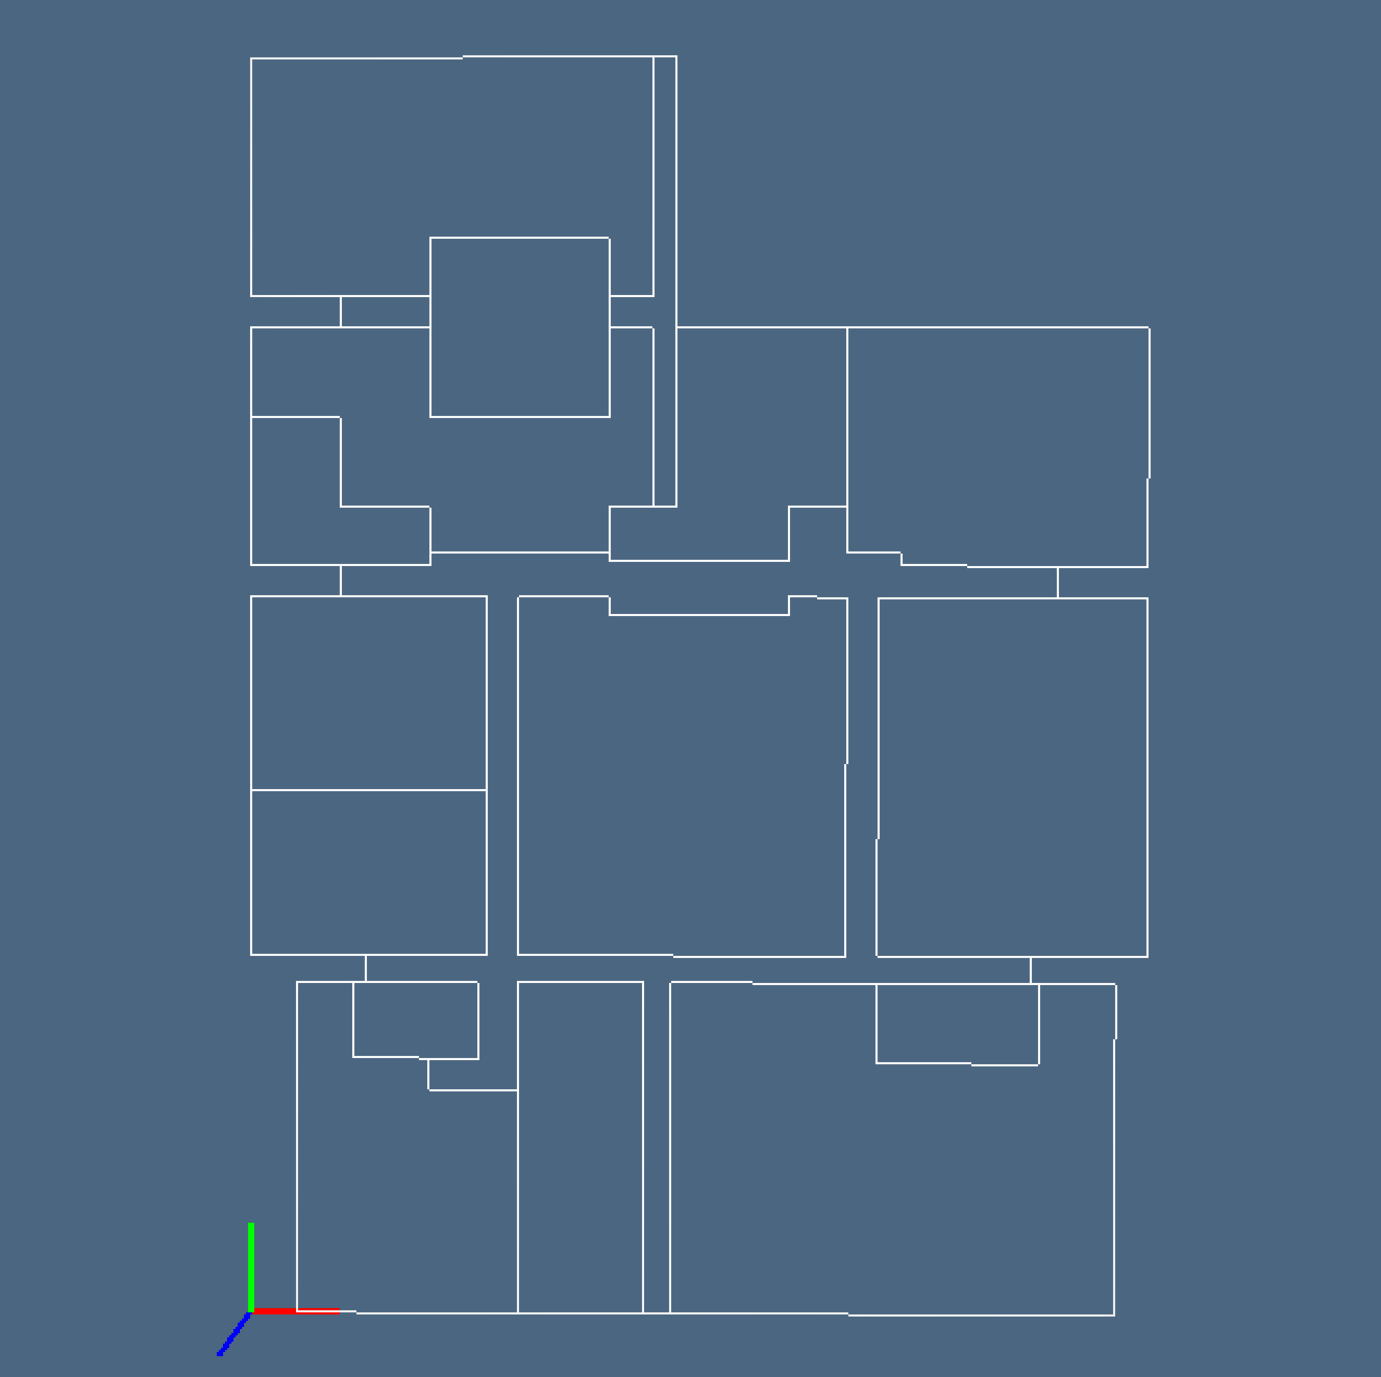
\includegraphics[height=0.329\linewidth,width=0.327\linewidth]{images/groundFloor1} 
   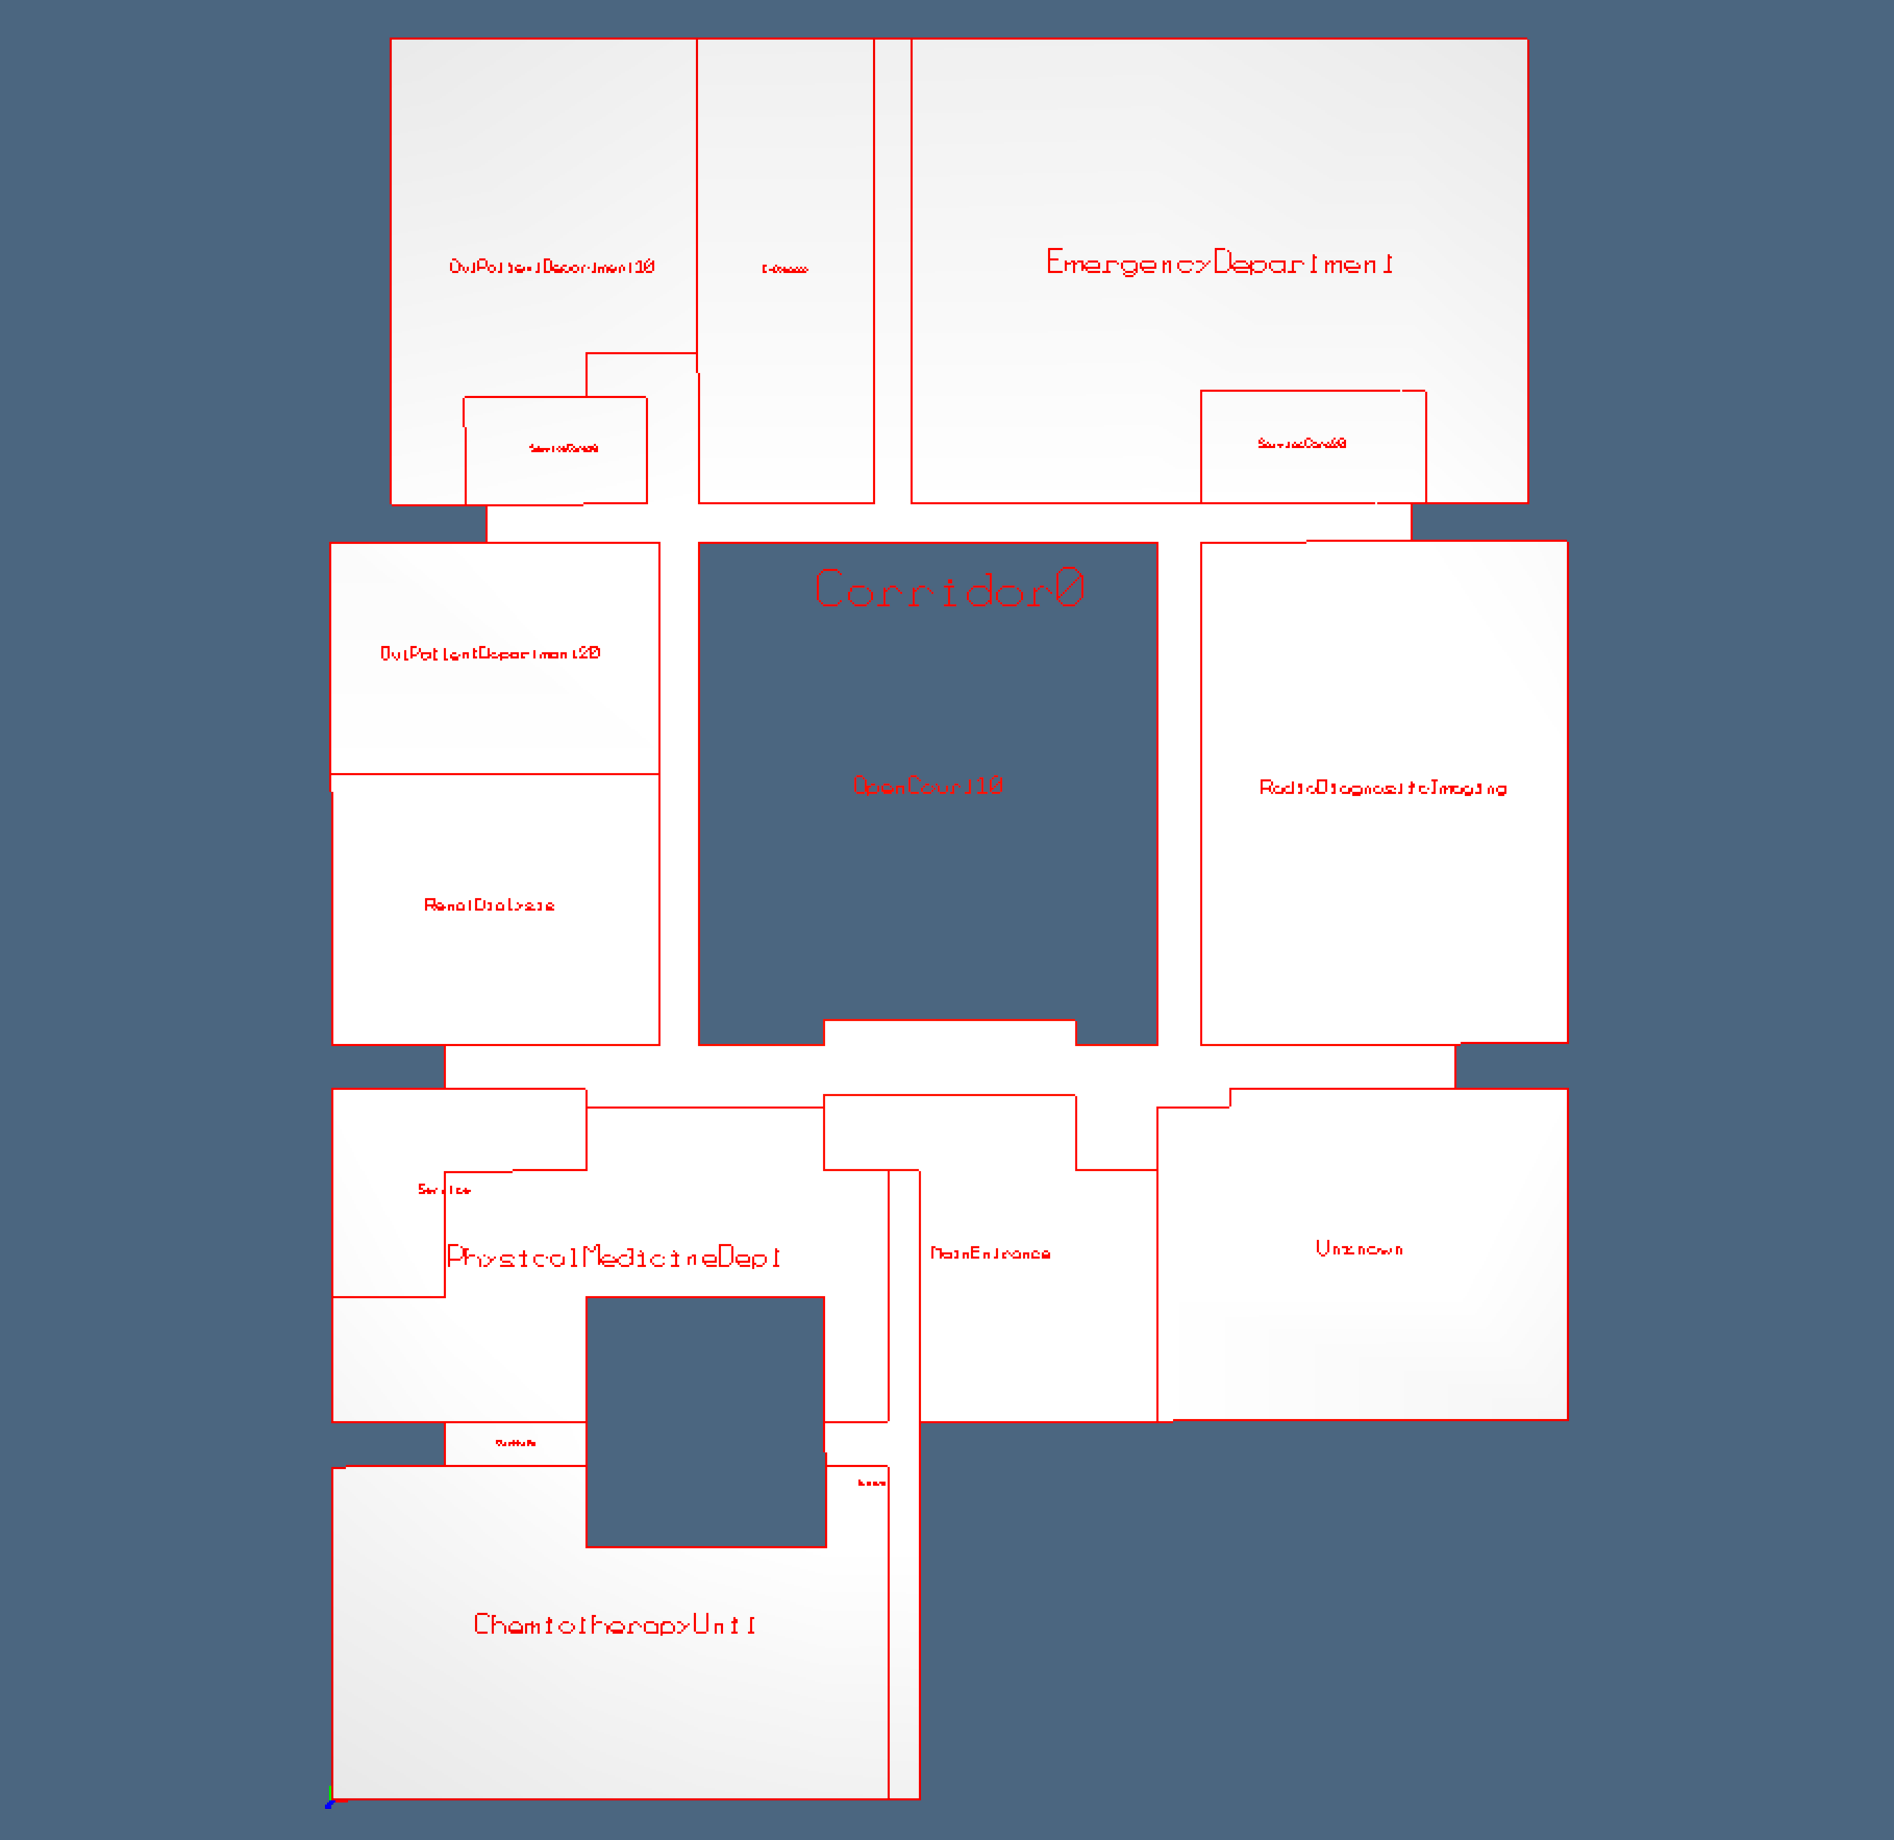
\includegraphics[height=0.329\linewidth,width=0.327\linewidth]{images/groundFloor} 
   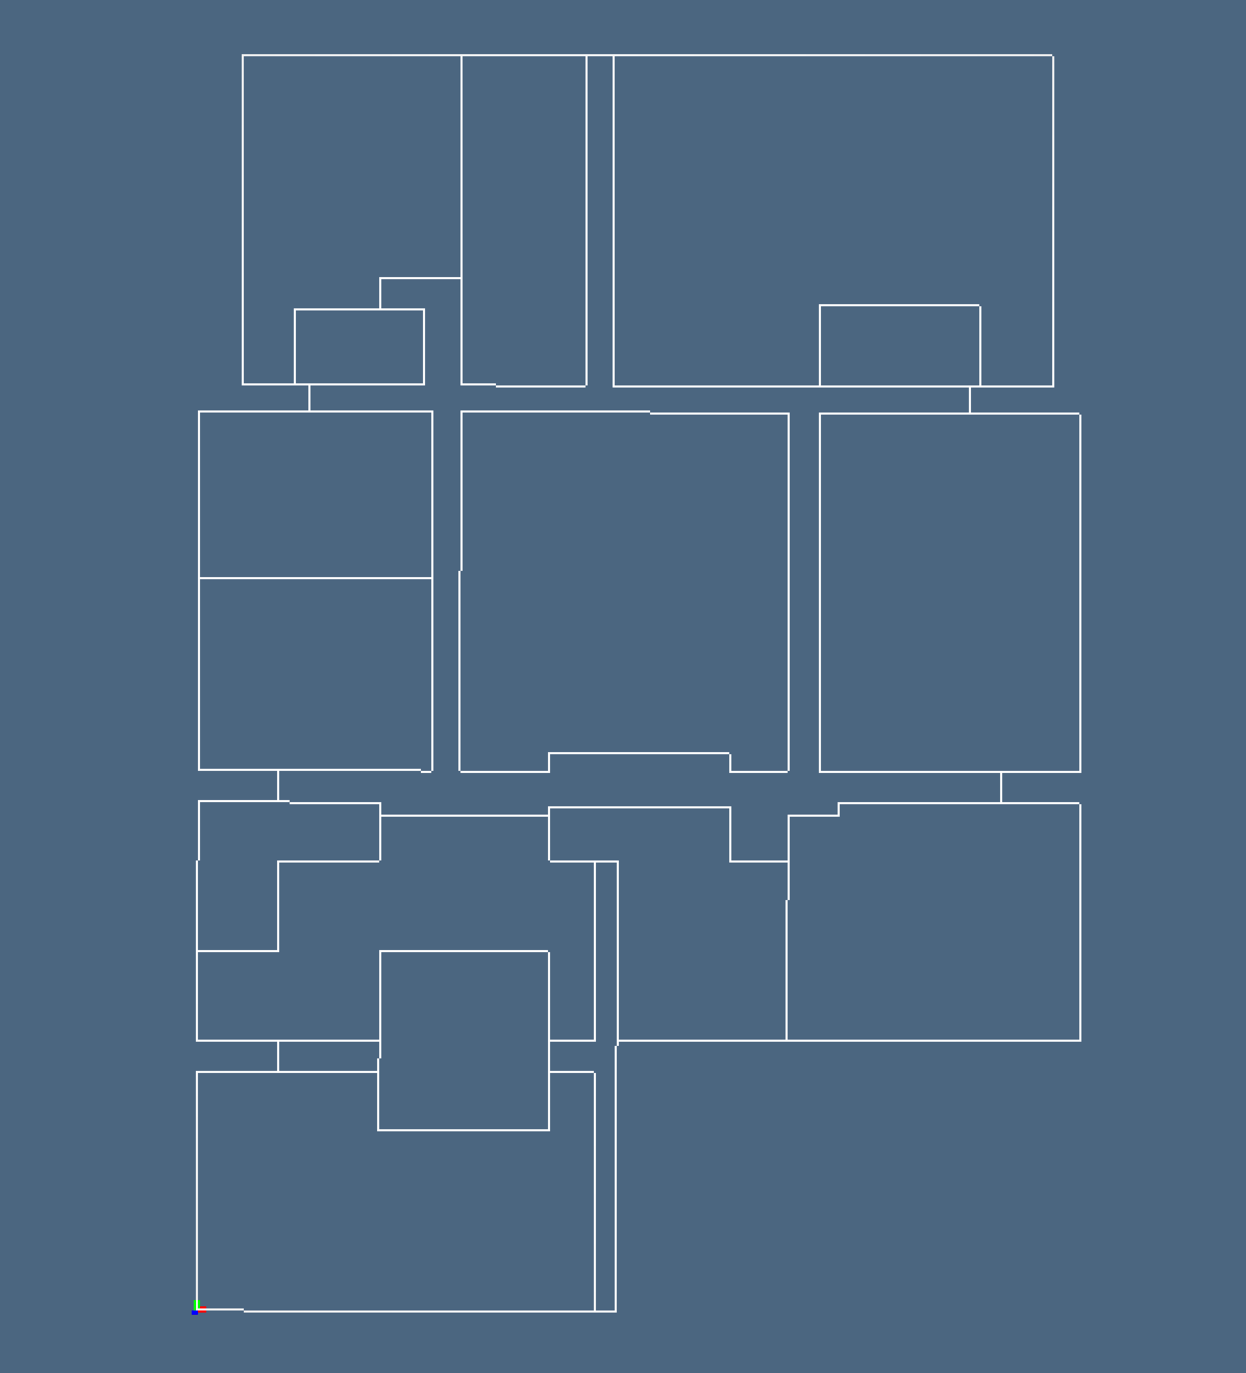
\includegraphics[height=0.329\linewidth,width=0.327\linewidth]{images/groundFloorMetric} 
   \caption{\texttt{groundFloor} images of (a) the 1-skeleton of its \texttt{LAR} representation, in grid coordinates; (b) component substructures in metric coordinates; (c) 1-skeleton. Notice the position and the scale of the reference frames.}
   \label{fig:groundFloor}
\end{figure}


\subsubsection{Mezanine floor}
\paragraph{Mezanine floor input}

%-------------------------------------------------------------------------------
@D Mezanine floor
@{""" Mezanine floor """
MedicalWaste = TRANS([[4./7.5,4./7.5,.8,1.25,1.25],[0,1.5,1.5,1.5,0]])
CentralStores = TRANS([[1.25,1.25,.8,.8,3.7,3.7,2.55,2.55,2.2,2.2],[0,1.5,1.5,
    2.65,2.65,.35,.35,.65,.65,0]])
StaffDining = TRANS([[3.95,3.95,6.7,6.7,6.95,6.95],[0,3.7,3.7,2,2,0]])
CSSD = TRANS([[6.95,6.95,6.95,8.8,8.8,9.65,9.65],[0,2,2.65,2.65,2,2,0]])
HouseKeeping = TRANS([[8.8,8.8,8.8,8.8,9.65,9.65],[2,2.65,2.8,3.7,3.7,2]])
CentralStaffChanging11 = TRANS([[4./7.5,4./7.5,1.15,1.15],[2.85,3.7,3.7,2.85]])
CentralStaffChanging21 = TRANS([[2.55,2.55,3.7,3.7],[2.85,3.7,3.7,2.85]])
OpenCourt11 = TRANS([[3,3,7,7,7],[4,8,8,6,4]])
Pharmacy = TRANS([[0,0,2.65,2.65,1.3],[4,6.45,6.45,4,4]])
CentralWorkshop = TRANS([[0,0,1,2.65,2.65],[6.45,8,8,8,6.45]])
Laundry = TRANS([[7,7,10,10,8.7],[4,6,6,4,4]])
AdministrationSuite11 = TRANS([[7,7,9,10,10],[6,8,8,8,6]])
MainLaboratories = TRANS([[1,1,0,0,2,2,5,5,4,4,4],[8.3,8.4,8.4,11,11,10,10,9,
    9,8.4,8.3]])
MedicalLibrary = TRANS([[6.7,6.7,8,8,7.75],[9.7,11,11,9.7,9.7]])
MedicalRecords = TRANS([[8,8,8,8.85,8.85,8.85],[8.3,9.7,11,11,9.75,8.3]])
AdministrationSuite21 = TRANS([[8.85,8.85,10,10,9,9],[8.3,9.75,9.75,8.4,8.4,8.3]])
MeetingRooms = TRANS([[6,6,6,6.7,6.7,7.75,7.75,7.45,7,7],[8.3,8.4,9,9,9.7,9.7,
    8.7,8.7,8.7,8.3]])
DataCenter = TRANS([[7,7,7.45,7.45],[8.3,8.7,8.7,8.3]])
ServerRoom = TRANS([[7.45,7.45,7.75,7.75],[8.3,8.7,8.7,8.3]])
PublicCore = TRANS([[4,4,5,6,6],[8.4,9,9,9,8.4]])
ServiceCore11 = TRANS([[1.15,1.15,1.3,2.55,2.55],[2.85,3.7,3.7,3.7,2.85]])
ServiceCore21 = TRANS([[7,7,8.7,8.8,8.8],[2.8,3.7,3.7,3.7,2.8]])
Corridor1 = [[2.2,0],[2.2,0.65],[2.55,0.65],[2.55,0.35],[3.7,0.35],[3.7,2.65],
    [0.8,2.65],[0.8,1.5],[0.5333,1.5],[0.5333,2.85],[1.15,2.85],[2.55,2.85],[3.7,
    2.85],[3.7,3.7],[2.55,3.7],[1.3,3.7],[1.3,4],[2.65,4],[2.65,6.45],[2.65,
    8],[1,8],[1,8.3],[4,8.3],[4,8.4],[6,8.4],[6,8.3],[7,8.3],[7.45,8.3],
    [7.75,8.3],[7.75,8.7],[7.75,9.7],[8,9.7],[8,8.3],[8.85,8.3],[9,8.3],[9,8],
    [7,8],[3,8],[3,4],[7,4],[8.7,4],[8.7,3.7],[7,3.7],[7,2.8],[8.8,2.8],
    [8.8,2.65],[6.95,2.65],[6.95,2],[6.7,2],[6.7,3.7],[3.95,3.7],[3.95,0]]
GroundRoof = TRANS([[4,4,2,2,1,1,0,0,4.75,4.75],[10,12,12,11,11,11.35,11.35,14,
    14,10]])
@}
%-------------------------------------------------------------------------------

\paragraph{Mezanine floor's building units}
%-------------------------------------------------------------------------------
@D Mezanine floor's building units 
@{""" Mezanine floor's building units """
medicalWaste = buildingUnit(MedicalWaste,"MedicalWaste")
centralStores = buildingUnit(CentralStores,"CentralStores")
staffDining = buildingUnit(StaffDining,"StaffDining")
cSSD = buildingUnit(CSSD,"CSSD")
houseKeeping = buildingUnit(HouseKeeping,"HouseKeeping")
centralStaffChanging11 = buildingUnit(CentralStaffChanging11,"CentralStaffChanging1")
centralStaffChanging21 = buildingUnit(CentralStaffChanging21,"CentralStaffChanging2")
openCourt11 = buildingUnit(OpenCourt11,"OpenCourt11") 
pharmacy = buildingUnit(Pharmacy,"Pharmacy")
centralWorkshop = buildingUnit(CentralWorkshop,"CentralWorkshop")
laundry = buildingUnit(Laundry,"Laundry")
administrationSuite11 = buildingUnit(AdministrationSuite11,"AdministrationSuite11")
mainLaboratories = buildingUnit(MainLaboratories,"MainLaboratories")
medicalLibrary = buildingUnit(MedicalLibrary,"MedicalLibrary")
medicalRecords = buildingUnit(MedicalRecords,"MedicalRecords")
administrationSuite21 = buildingUnit(AdministrationSuite21,"AdministrationSuite21")
meetingRooms = buildingUnit(MeetingRooms,"MeetingRooms")
dataCenter = buildingUnit(DataCenter,"DataCenter")
serverRoom = buildingUnit(ServerRoom,"ServerRoom")
publicCore = buildingUnit(PublicCore,"PublicCore")
serviceCore11 = buildingUnit(ServiceCore11,"ServiceCore11")
serviceCore21 = buildingUnit(ServiceCore21,"ServiceCore21")
corridor1 = buildingUnit(Corridor1,"Corridor1")
groundRoof = buildingUnit(GroundRoof,"GroundRoof")
@}
%-------------------------------------------------------------------------------

\begin{figure}[htbp] %  figure placement: here, top, bottom, or page
   \centering
   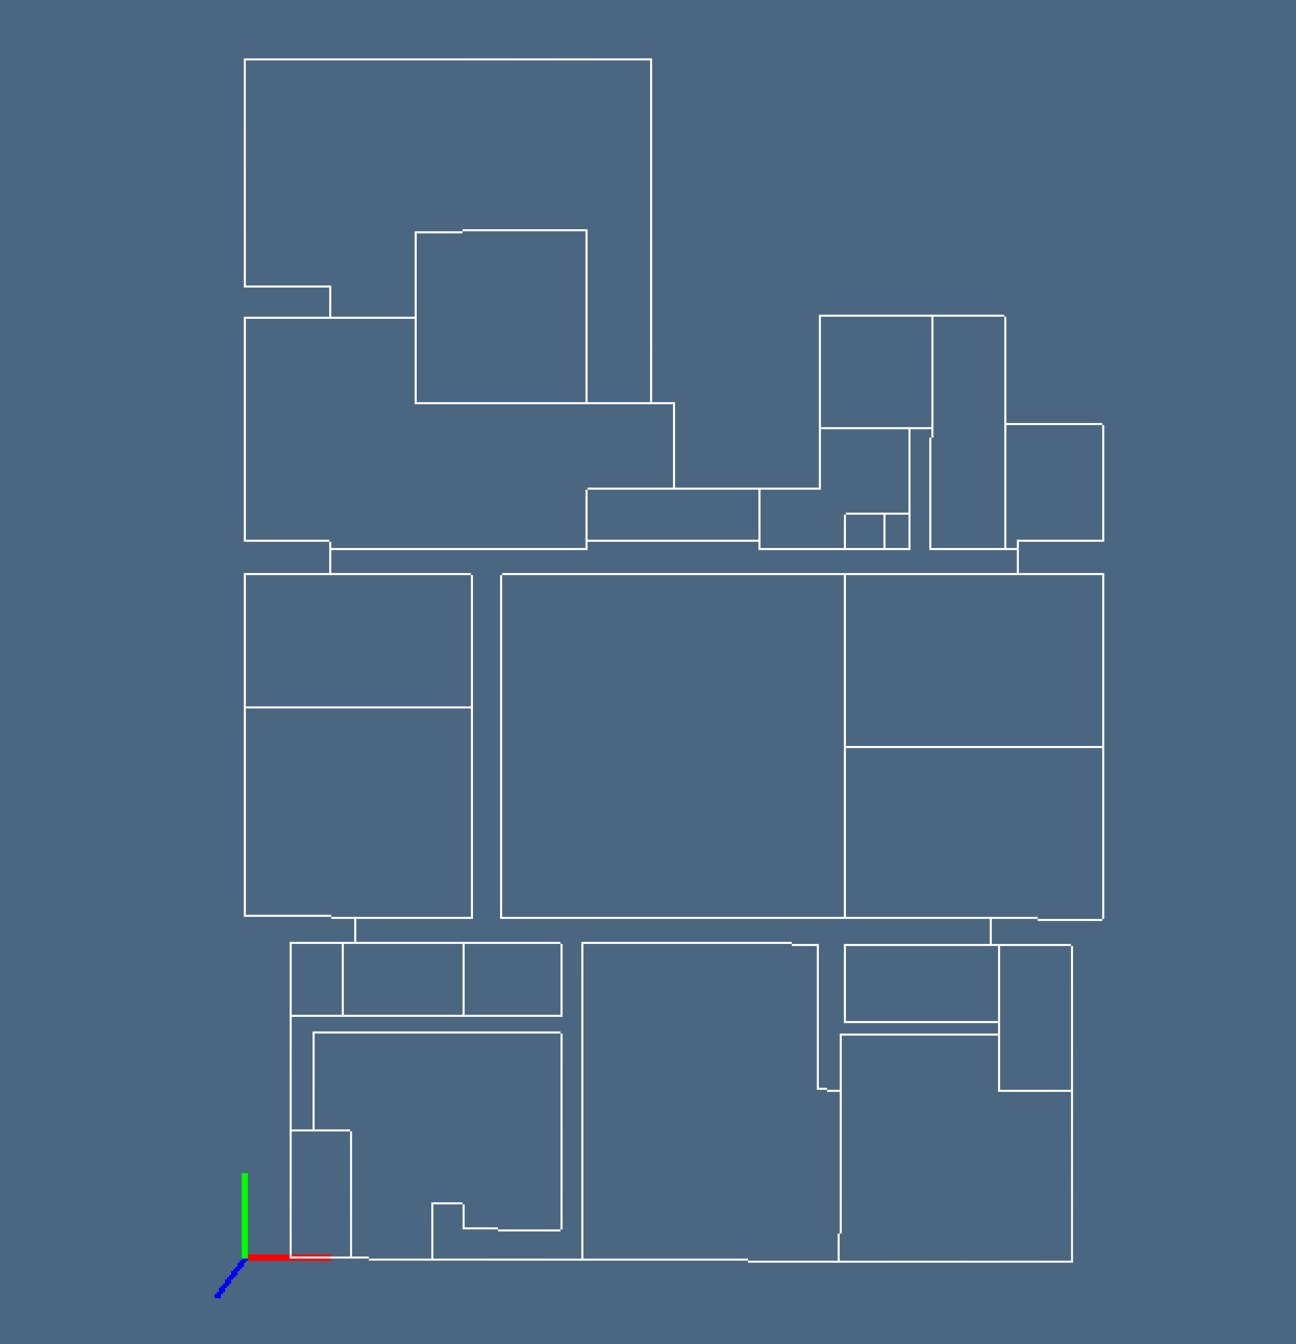
\includegraphics[height=0.329\linewidth,width=0.327\linewidth]{images/mezanineFloor1} 
   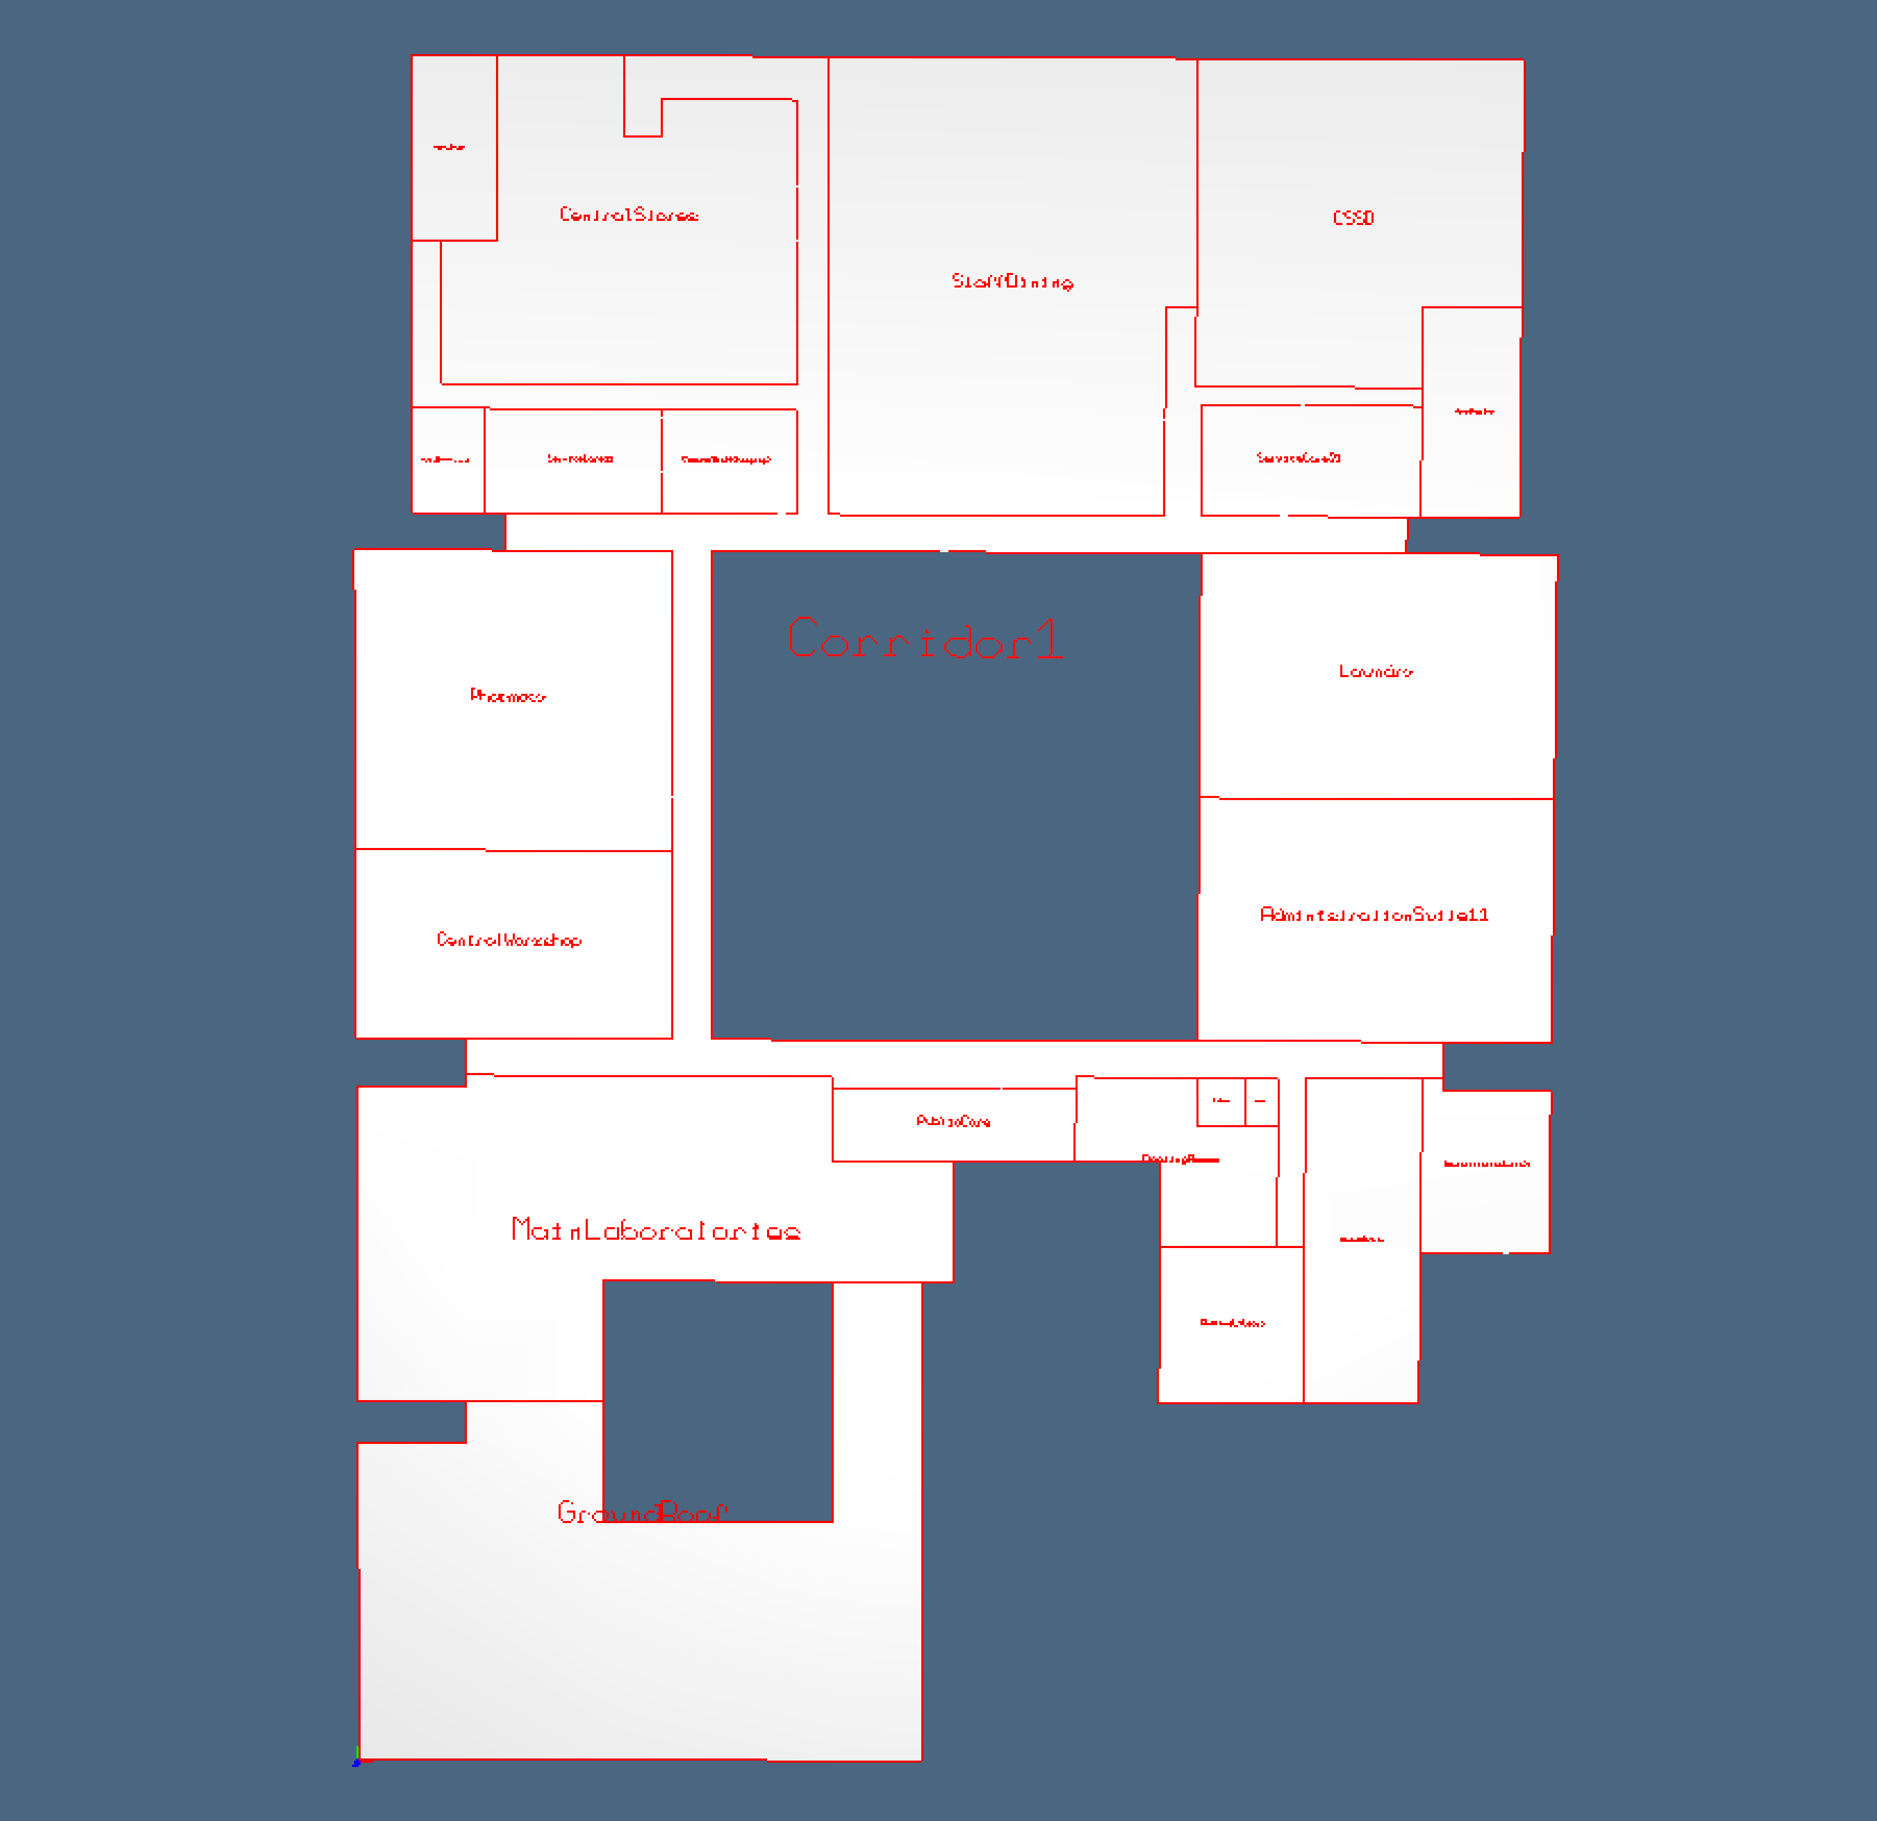
\includegraphics[height=0.329\linewidth,width=0.327\linewidth]{images/mezanineFloor} 
   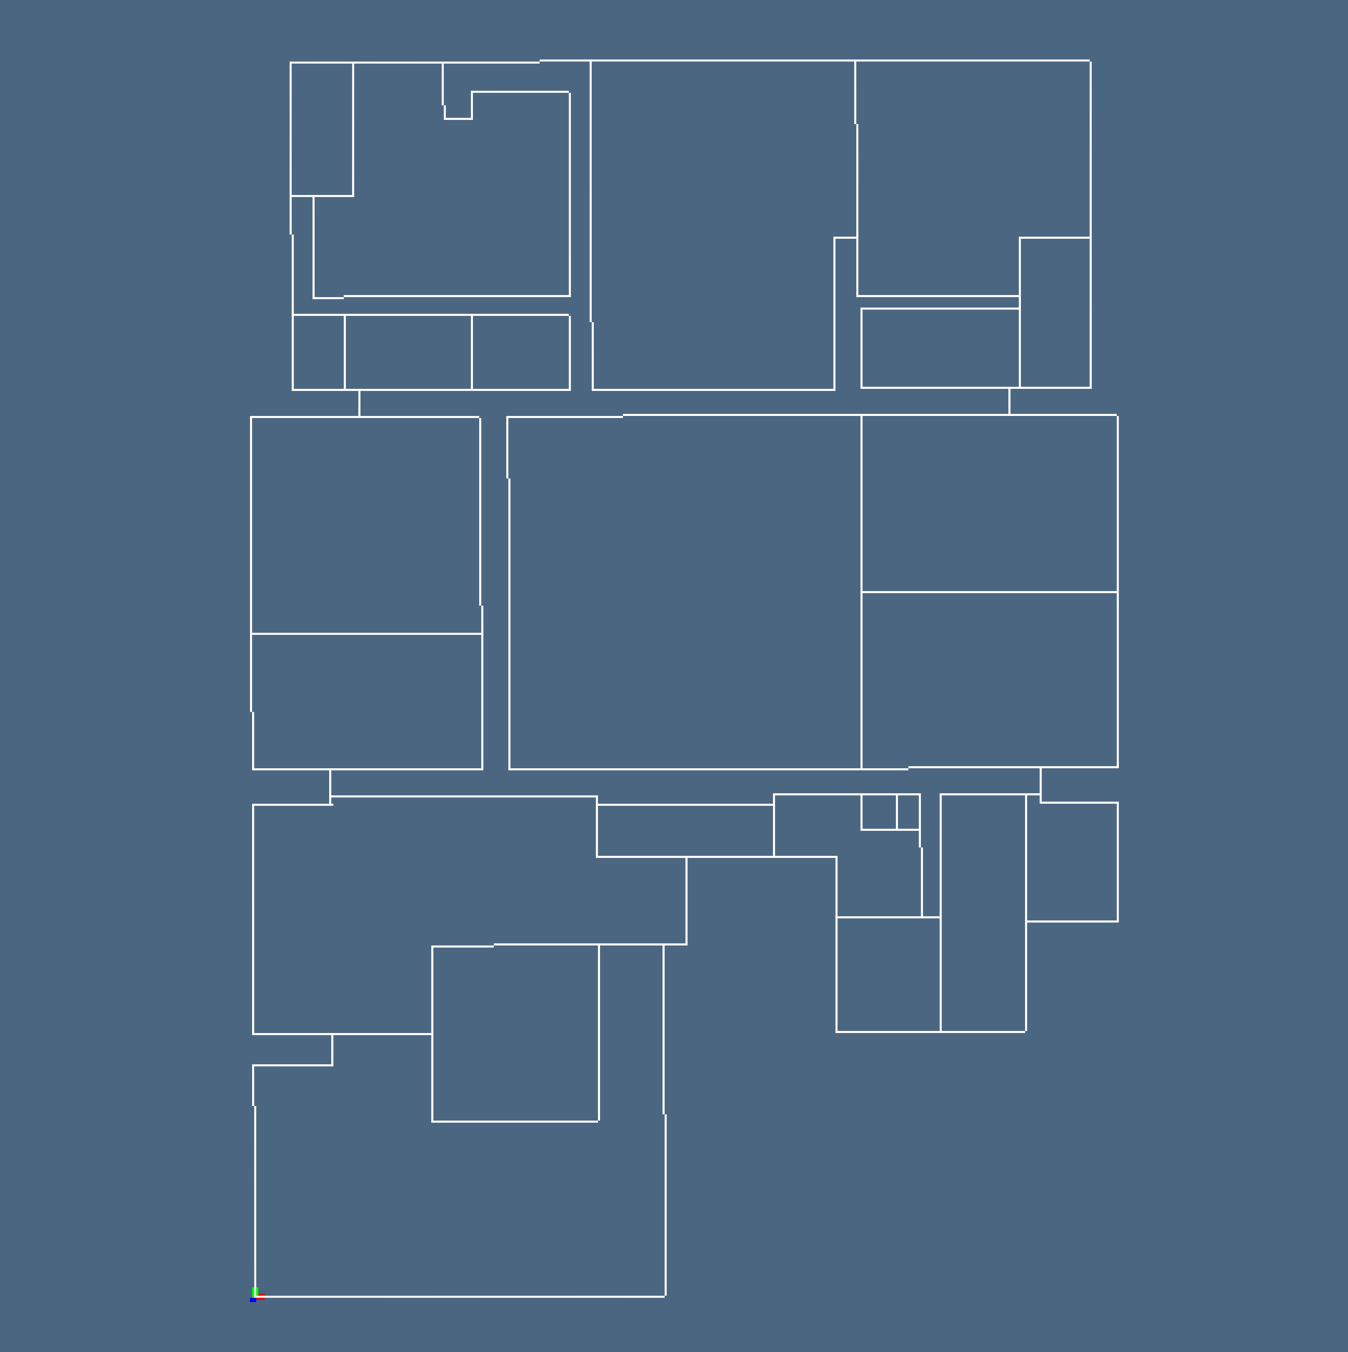
\includegraphics[height=0.329\linewidth,width=0.327\linewidth]{images/mezanineFloor2} 
   \caption{\texttt{mezanineFloor} images of (a) the 1-skeleton of its \texttt{LAR} representation, in grid coordinates; (b) component substructures in metric coordinates; (c) 1-skeleton. Notice the position and the scale of the reference frames.}
   \label{fig:mezanine}
\end{figure}

%-------------------------------------------------------------------------------
@D Mezanine floor structure
@{""" Mezanine floor structure """

@< Mezanine floor's building units @>

buildingUnits1 = [medicalWaste, centralStores, staffDining, cSSD, houseKeeping, 
    centralStaffChanging11, centralStaffChanging21, pharmacy, centralWorkshop, laundry, 
    administrationSuite11, mainLaboratories, medicalLibrary, medicalRecords, 
    administrationSuite21, meetingRooms, dataCenter, serverRoom, publicCore, 
    serviceCore11, serviceCore21, corridor1, groundRoof]
    
mezanineFloor = Struct(buildingUnits1, "mezanineFloor")
@}
%-------------------------------------------------------------------------------


\subsubsection{First floor}
\paragraph{First floor}
%-------------------------------------------------------------------------------
@D First floor
@{""" First floor """
OpenCourt3 = TRANS([[3.,3.,7.,7.],[4.,8.,8.,4.]])
Surgery = TRANS([[4.15,4.15,7.,7.,8.8,8.8,9.65,9.65],[0,3.7,3.7, 2.8,2.8, 3.7,3.7,0]])
CatheterizationLab = TRANS([[3,3,4.15,4.15],[0,3.7,3.7,0]])
ServiceCore32 = TRANS([[7.,7.,8.7,8.8,8.8],[2.8,3.7,3.7,3.7,2.8]])
CoronaryCareUnit = TRANS([[7.,7.,8.3,9.,10.,10.,8.7],[4.,8.,8.,8.,8.,4.,4.]])
DeliveryAndNicu = TRANS([[0,0, 1.7,2.65,2.65,1.3],[4.,8.,8.,8.,4.,4.]])
ServiceCore31 = TRANS([[1.15, 1.15, 1.3,2.65, 2.65], [2.85, 3.7,3.7, 3.7, 2.85]])
IntensiveCareUnit = TRANS([[4./7.5, 4./7.5,1.15,1.15,2.65, 2.65,1.95,1.95],
    [0.,3.7,3.7,2.85,2.85,.6,.6,0.]])
ServiceCore33 = TRANS([[1.95,1.95,2.65, 2.65],[0,.6,.6,0]])
PublicCore3 = TRANS([[1.7,1.7,4.,4.,6.,6.,8.3,8.3,7,3,2.65],
    [8,8.4,8.4,9,9,8.4,8.4,8,8,8,8]])
Corridor3 = TRANS([[2.65,2.65,2.65,2.65,1.3,1.3,2.65,2.65,3.0,3.0,7.0,8.7,8.7,
    7.0,4.15,3.0,3.0],[0.0,0.6,2.85,3.7,3.7,4.0,4.0,8.0,8.0,4.0,4.0,4.0,3.7,
    3.7,3.7,3.7,0.0]])
MezanineRoof = TRANS([[1,1,0,0,2,2,4.75,4.75,10,10,9,9,8.3,8.3, 6,6,4,4 ,1.7,1.7],
    [8,8.4,8.4,11,11,10,10,11,11,8.4,8.4,8,8,8.4,8.4,9,9,8.4,8.4,8]])
@}
%-------------------------------------------------------------------------------

\paragraph{First floor's building units}
%-------------------------------------------------------------------------------
@D First floor's building units 
@{""" First floor's building units """
openCourt3 = buildingUnit(OpenCourt3,"OpenCourt3")
surgery = buildingUnit(Surgery,"Surgery")
catheterizationLab = buildingUnit(CatheterizationLab,"CatheterizationLab")
serviceCore32 = buildingUnit(ServiceCore32,"ServiceCore32")
coronaryCareUnit = buildingUnit(CoronaryCareUnit,"CoronaryCareUnit")
deliveryAndNicu = buildingUnit(DeliveryAndNicu,"DeliveryAndNicu")
serviceCore31 = buildingUnit(ServiceCore31,"ServiceCore31")
intensiveCareUnit = buildingUnit(IntensiveCareUnit,"IntensiveCareUnit")
serviceCore33 = buildingUnit(ServiceCore33,"ServiceCore33")
publicCore3 = buildingUnit(PublicCore3,"PublicCore3")
corridor3 = buildingUnit(Corridor3,"Corridor3")
mezanineRoof = buildingUnit(MezanineRoof,"MezanineRoof")
@}
%-------------------------------------------------------------------------------

\begin{figure}[htbp] %  figure placement: here, top, bottom, or page
   \centering
   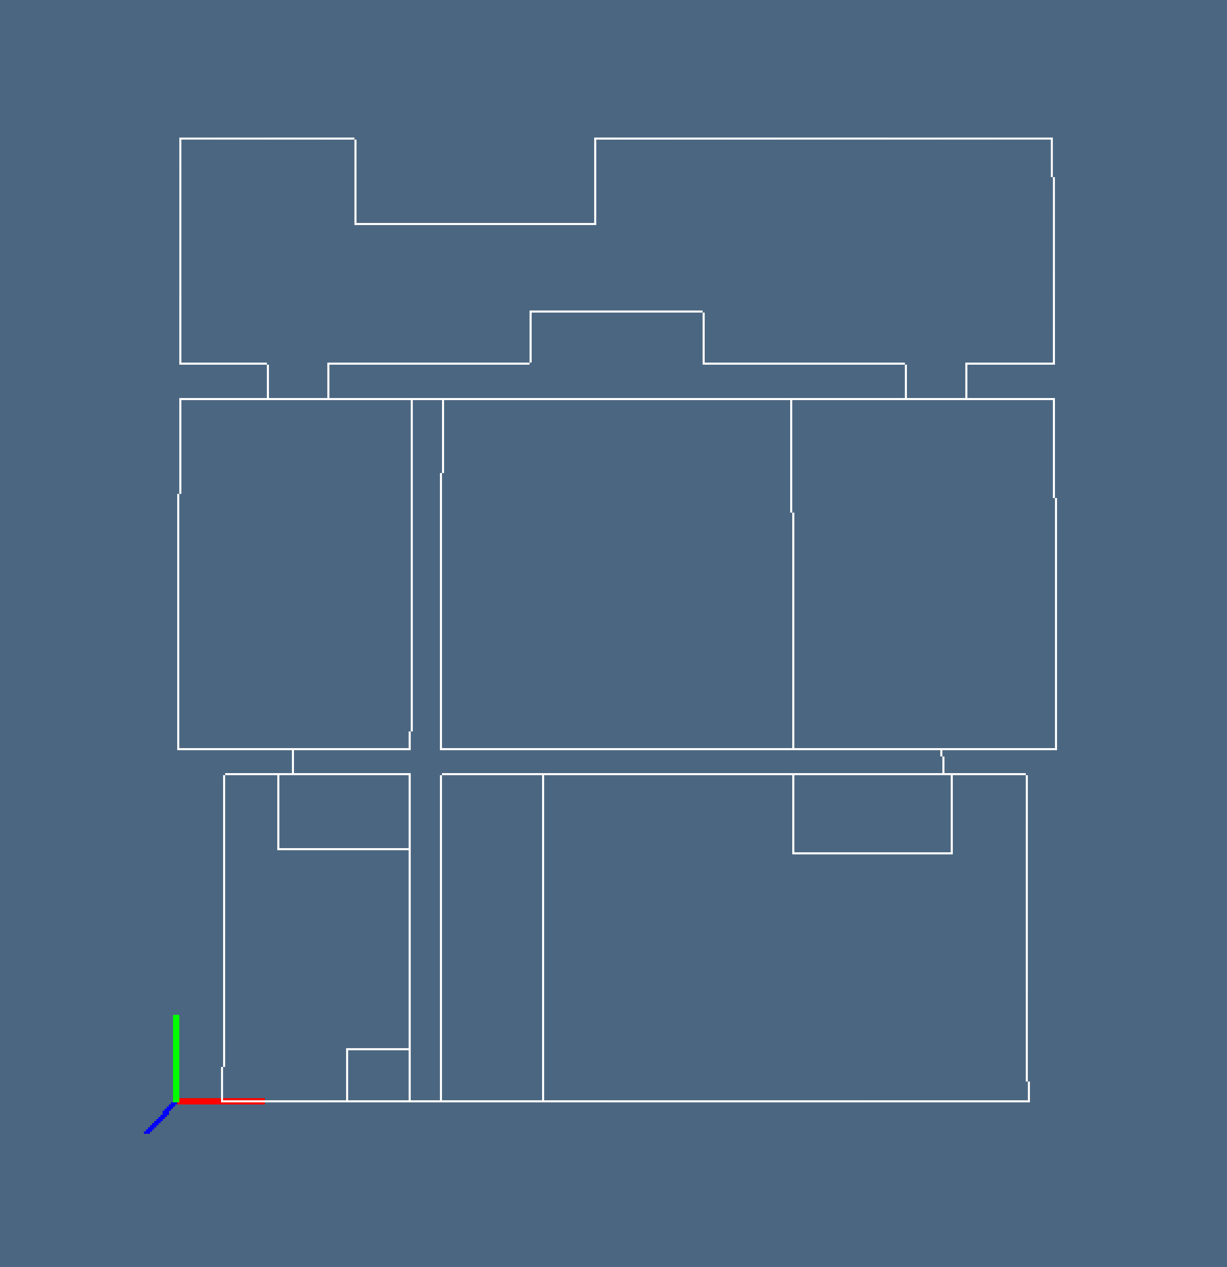
\includegraphics[height=0.329\linewidth,width=0.327\linewidth]{images/firstFloor2Hospital} 
   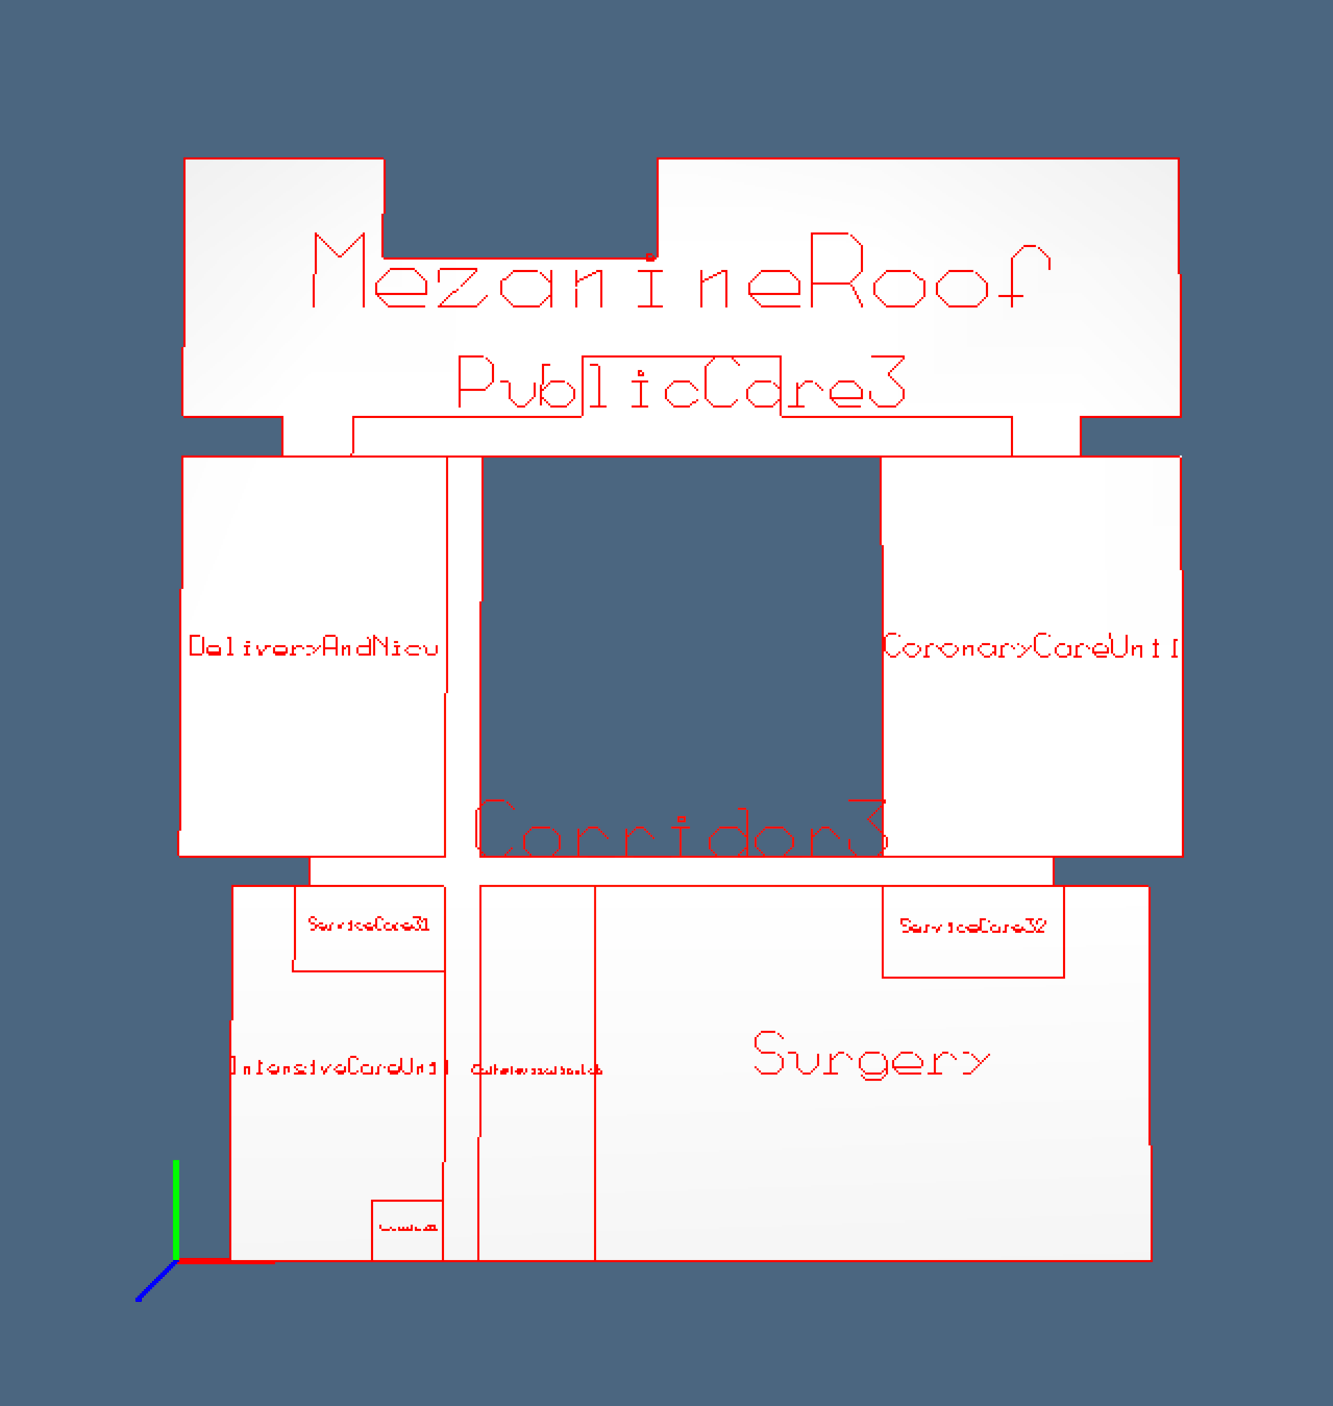
\includegraphics[height=0.329\linewidth,width=0.327\linewidth]{images/firstFloorHospital} 
   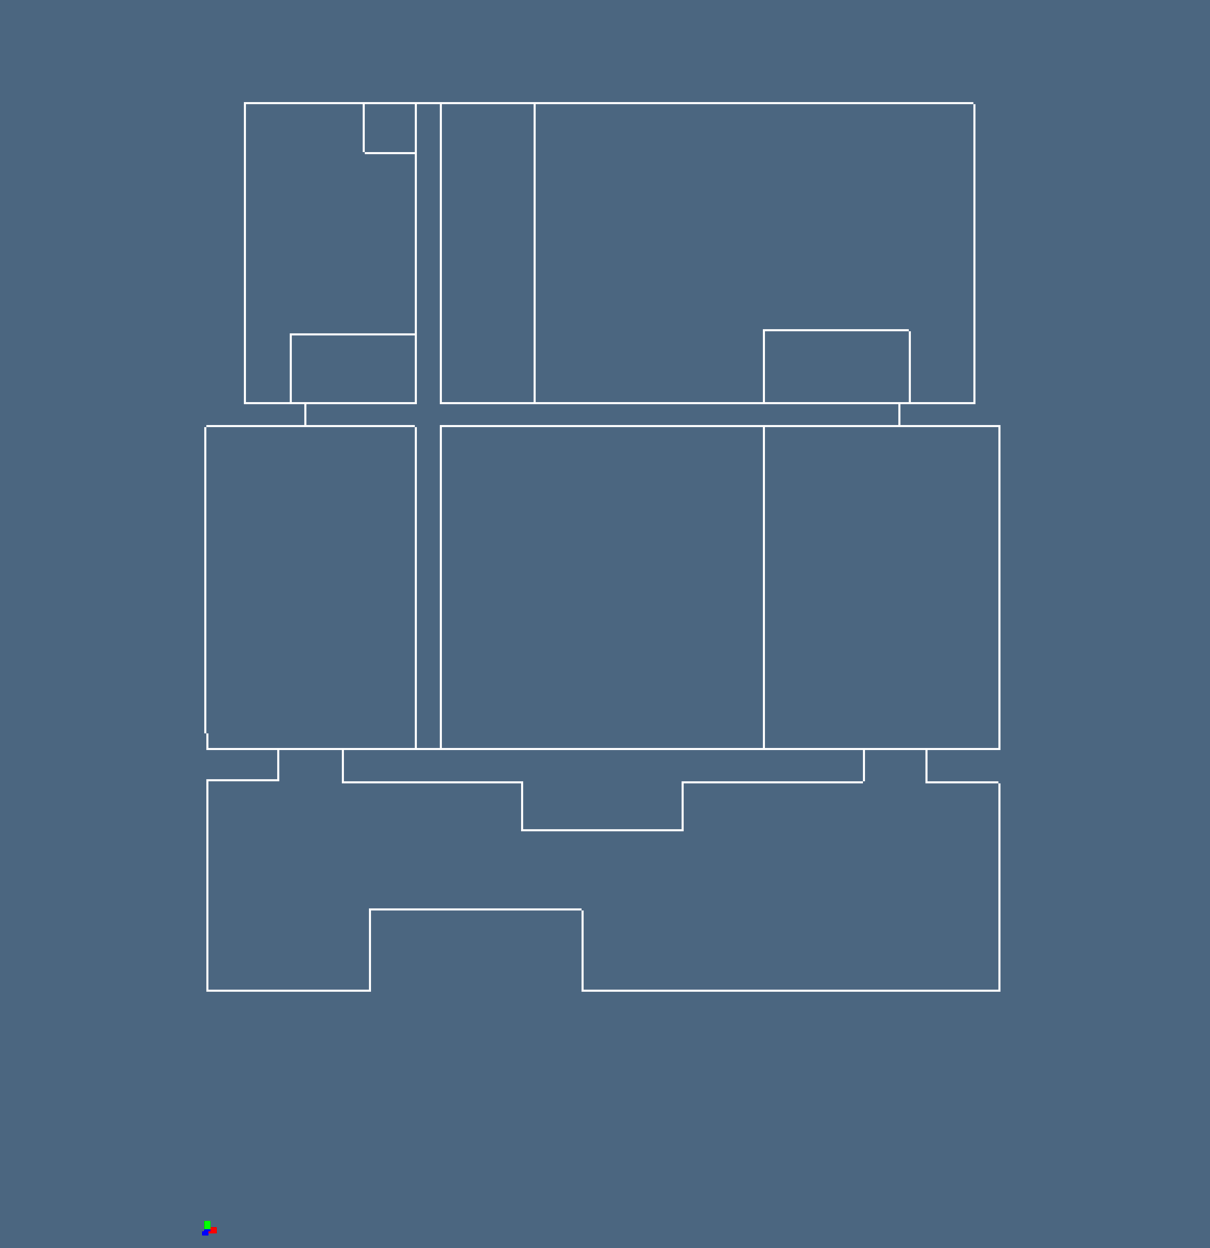
\includegraphics[height=0.329\linewidth,width=0.327\linewidth]{images/firstFloor2} 
   \caption{\texttt{firstFloor} images of (a) the 1-skeleton of its \texttt{LAR} representation, in grid coordinates; (b) component substructures in metric coordinates; (c) 1-skeleton. Notice the position and the scale of the reference frames.}
   \label{fig:firstFloor}
\end{figure}

%-------------------------------------------------------------------------------
@D First floor structure
@{""" First floor structure """

@< First floor's building units @>

buildingUnits2 = [surgery,catheterizationLab,serviceCore32,coronaryCareUnit,
    deliveryAndNicu,serviceCore31,intensiveCareUnit,serviceCore33,publicCore3,
    corridor3,mezanineRoof]
    
firstFloor = Struct(buildingUnits2, "firstFloor")
@}
%-------------------------------------------------------------------------------


\subsubsection{Ward sections}
\paragraph{Ward sections}
Here input by polylines and structure modeling are freely mixed. Just notice that
the affine maps included in structures are given in grid coordinates. This fact 
does not permit an immediate transformation in Cartesian coordinates using the \texttt{metric}
function.
%-------------------------------------------------------------------------------
@D Ward sections
@{""" Ward sections """
Room = polyline2lar([TRANS([[0,0,1,1,2./3,2./3],[0,0.5,0.5,0.25,0.25,0]])])
RestRoom = polyline2lar([TRANS([[2./3,2./3,1,1],[0,0.25,0.25,0]])])
Nursing1 = polyline2lar([TRANS([[0,0,.2,.2],[0,.4,.4,.0]])])
Nursing2 = polyline2lar([TRANS([[.2,.2,.4,.4],[0,.4,.4,.0]])])
Nursing3 = polyline2lar([TRANS([[0,0,.4,.4,.2],[.4,.8,.8,.4,.4]])])
Nursing4 = polyline2lar([TRANS([[0,0,.4,.4],[.8,1.1,1.1,.8]])])
Nursing5 = polyline2lar([TRANS([[0,0,.4,.4],[1.1,1.4,1.4,1.1]])])

room = Struct([Room],"Room")
restRoom = Struct([RestRoom],"RestRoom")
nursing1 = Struct([Nursing1],"Nursing1")
nursing2 = Struct([Nursing2],"Nursing2")
nursing3 = Struct([Nursing3],"Nursing3")
nursing4 = Struct([Nursing4],"Nursing4")
nursing5 = Struct([Nursing5],"Nursing5")

service1 = Struct([nursing1,nursing2,nursing3,nursing4,nursing5],"Service1")
service2 = Struct([t(0,1.4),s(1,-1),service1],"Service2")
wardServices = Struct([t(1.3,.3),service2,t(0,2),service1],"WardServices")
theRoom = Struct([room,restRoom],"TheRoom")
twoRooms =  Struct([theRoom,t(0,1),s(1,-1),theRoom],"TwoRooms")
halfWard = Struct(4*[twoRooms,t(0,1)],"HalfWard")
ward = Struct([halfWard, wardServices, t(3,0),s(-1,1), halfWard],"Ward")
V,FV,EV = struct2lar(ward)
theWard = lar2lines((V,FV))
@}
%-------------------------------------------------------------------------------

\begin{figure}[htbp] %  figure placement: here, top, bottom, or page
   \centering
   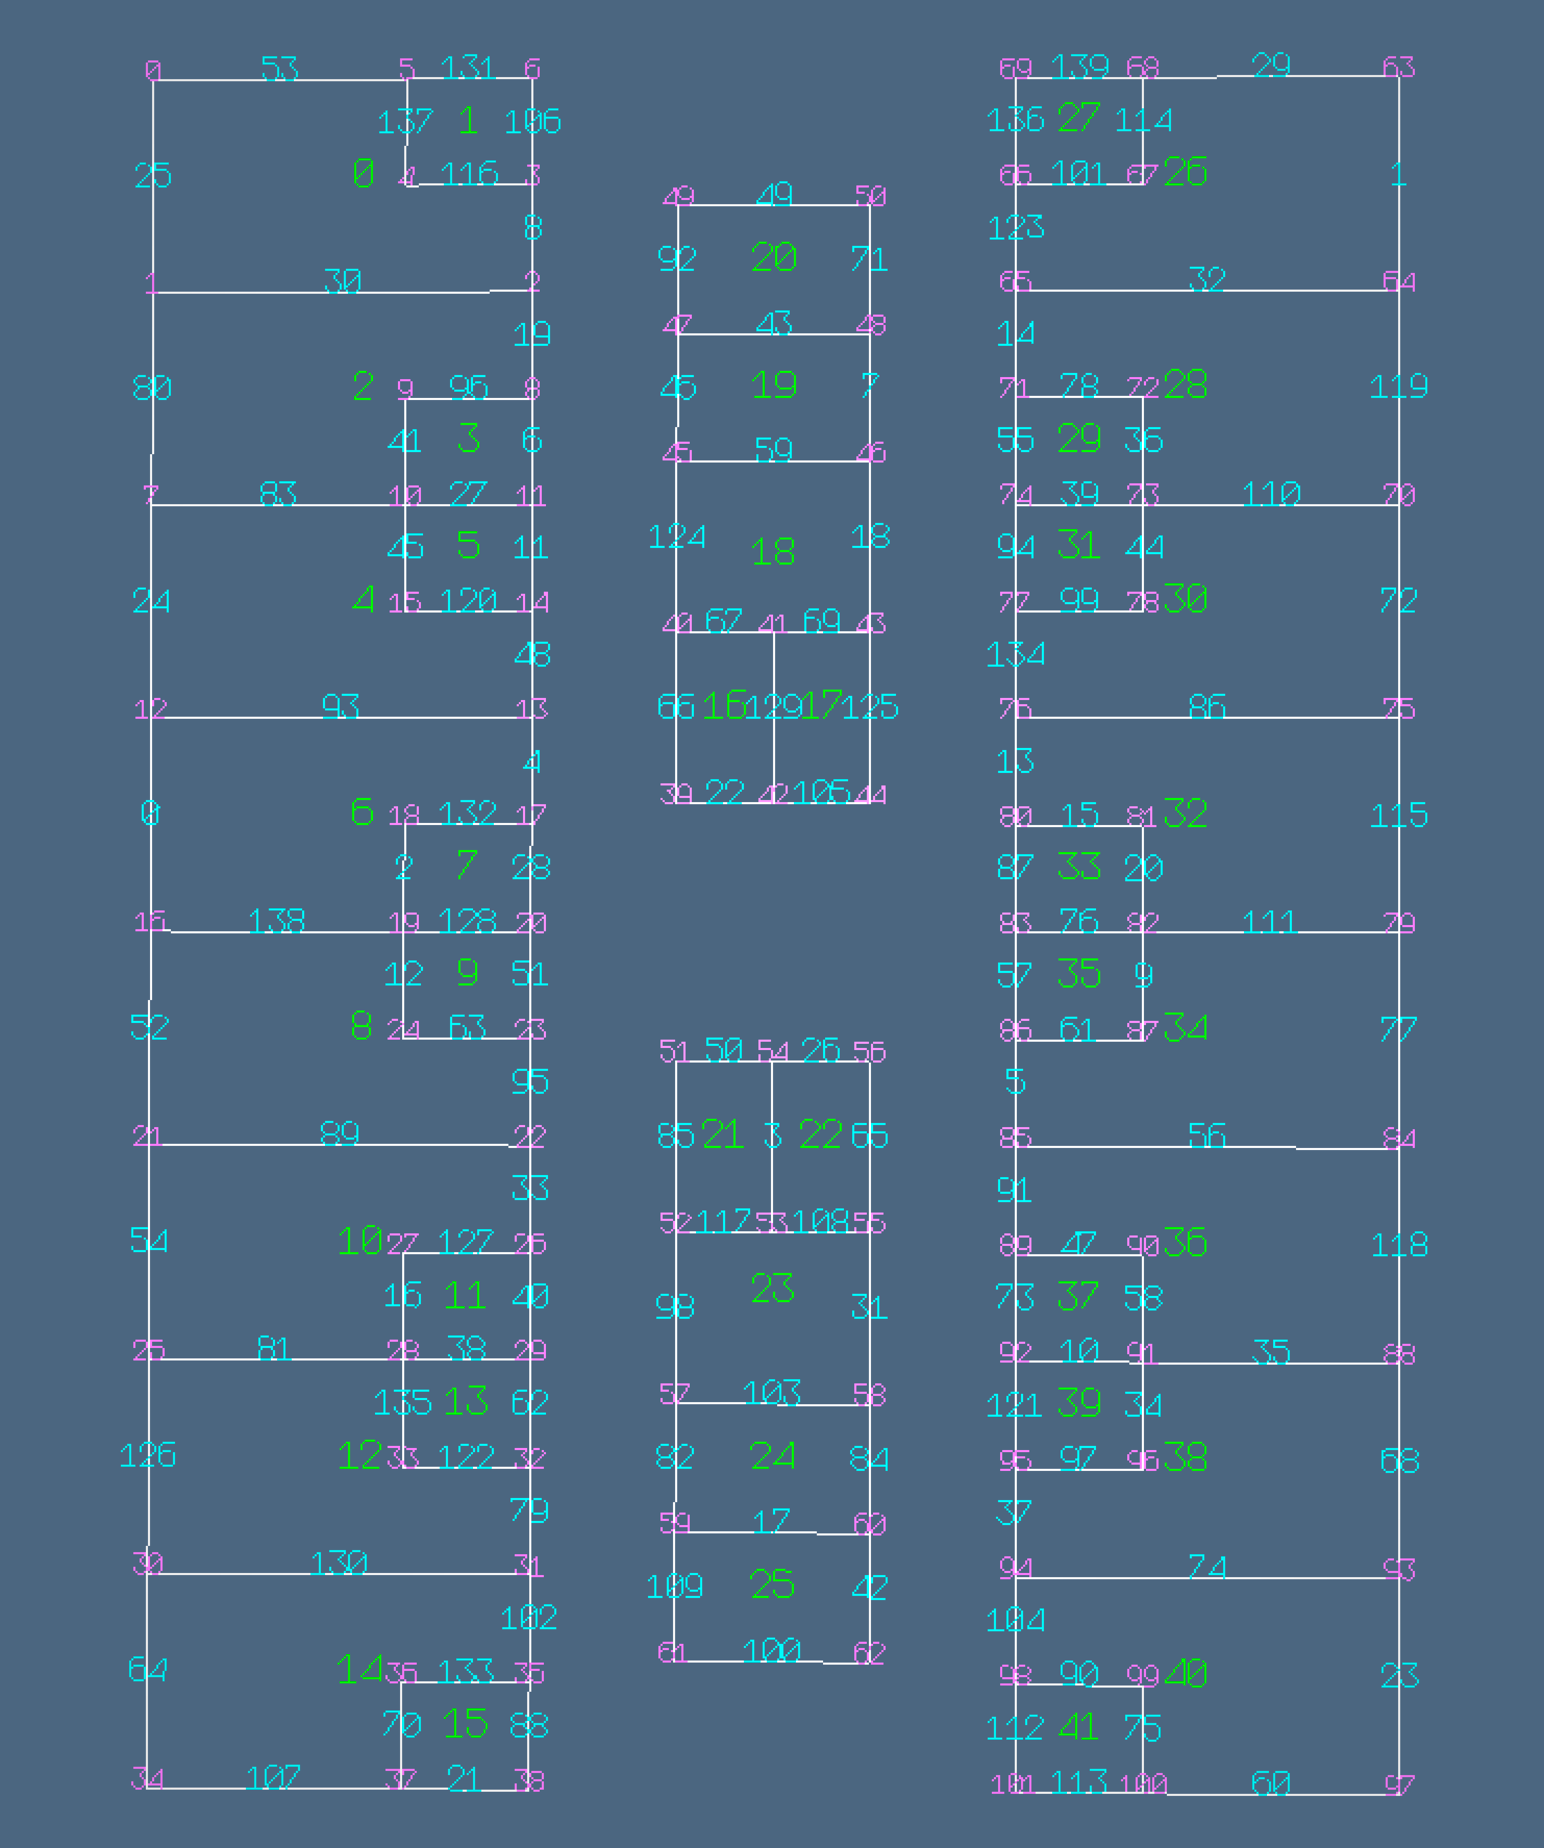
\includegraphics[width=0.5\linewidth]{images/ward} 
   \caption{The cellular complex $(V,FV,EV)$ generated by the \texttt{ward} structure.}
   \label{fig:ward}
\end{figure}


\subsubsection{Second floor}
\paragraph{Second floor} 
%-------------------------------------------------------------------------------
@D Second floor
@{
@< Ward sections @>

""" Second floor """
PublicCore4 = TRANS([[1.7,1.7,4,4,6,6,8.3,8.3, 8,7+2./3, 7, 3, 2+1./3,2],
    [8,8.4,8.4,9,9,8.4,8.4,8,8,8,8,8,8,8]])
Filter1 = TRANS([[1,1,1.35,1.35,1.15],[3.7,4,4,3.7,3.7]])
Filter2 = TRANS([[8.65,8.65,9,9,8.8],[3.7,4,4,3.7,3.7]])
ServiceCore14 = TRANS([[1.15, 1.15, 1.35,2.55, 2.55], [2.8, 3.7,3.7, 3.7, 2.8]])
ServiceCore24 = TRANS([[7,7,8.65,8.8,8.8],[2.8,3.7,3.7,3.7,2.8]])
FirstRoof = TRANS([[4./7.5, 4./7.5,1.15,1.15,2.55,2.55,7,7,8.8,8.8,9.65,9.65],
    [0,3.7,3.7,2.8,2.8,3.7,3.7,2.8,2.8,3.7,3.7,0]])
Corridor4a = [[1.35,3.7],[1.35,4],[2,4],[2.3333,4],[3,4],[7,4],[7.6667,4],[8,4],
    [8.65,4],[8.65,3.7],[7,3.7],[2.55,3.7]]
Corridor4b = [[1,4.0],[1,4.25],[1,4.5],[1,4.75],[1,5.0],[1,5.25],[1,5.5],
    [1,5.75],[1,6.0],[1,6.25],[1,6.5],[1,6.75],[1,7.0],[1,7.25],[1,7.5],
    [1,7.75],[1,8.0],[2,8.0],[2,7.75],[2,7.5],[2,7.25],[2,7.0],[2,6.75],
    [2,6.5],[2,6.25],[2,6.0],[2,5.75],[2,5.5],[2,5.25],[2,5.0],[2,4.75],
    [2,4.5],[2,4.25],[2,4.0],[1.35,4.0]]
Corridor4b1 = [[1.3,4.3],[1.3,4.6],[1.3,4.9],[1.3,5.3],[1.3,5.7],[1.5,5.7],[1.7,5.7],
    [1.7,5.3],[1.7,4.9],[1.7,4.6],[1.7,4.3]]
Corridor4b2 = [[1.3,6.3],[1.3,6.7],[1.3,7.1],[1.3,7.4],[1.3,7.7],[1.7,7.7],[1.7,7.4],
    [1.7,7.1],[1.7,6.7],[1.7,6.3],[1.5,6.3]]
Corridor4c = [[8,4.0],[8,4.25],[8,4.5],[8,4.75],[8,5.0],[8,5.25],[8,5.5],
    [8,5.75],[8,6.0],[8,6.25],[8,6.5],[8,6.75],[8,7.0],[8,7.25],[8,7.5],
    [8,7.75],[8,8.0],[8.3,8.0],[9,8.0],[9,7.75],[9,7.5],[9,7.25],[9,7.0],
    [9,6.75],[9,6.5],[9,6.25],[9,6.0],[9,5.75],[9,5.5],[9,5.25],[9,5.0],
    [9,4.75],[9,4.5],[9,4.25],[9,4.0],[8.65,4.0]]
Corridor4c1 = [[8.3,4.3],[8.3,4.6],[8.3,4.9],[8.3,5.3],[8.3,5.7],[8.5,5.7],[8.7,5.7],
    [8.7,5.3],[8.7,4.9],[8.7,4.6],[8.7,4.3]]
Corridor4c2 = [[8.3,6.3],[8.3,6.7],[8.3,7.1],[8.3,7.4],[8.3,7.7],[8.7,7.7],[8.7,7.4],
    [8.7,7.1],[8.7,6.7],[8.7,6.3],[8.5,6.3]]
@}
%-------------------------------------------------------------------------------

\paragraph{Second floor's building units}
%-------------------------------------------------------------------------------
@D Second floor's building units 
@{""" Second floor's building units """
publicCore4 = buildingUnit(PublicCore4,'PublicCore4')
ward21 = deepcopy(ward)
ward22 = deepcopy(ward)
obstetricGinecologicWard = Struct([t(0,4),ward21],'ObstetricGinecologicWard')
surgicalWard1 = Struct([t(7,4),ward22],'SurgicalWard1')
filter1 = buildingUnit(Filter1,'Filter1')
filter2 = buildingUnit(Filter2,'Filter2')
serviceCore14 = buildingUnit(ServiceCore14,'ServiceCore14')
serviceCore24 = buildingUnit(ServiceCore24,'ServiceCore24')
firstRoof = buildingUnit(FirstRoof,'FirstRoof')
serviceCore11 = buildingUnit(ServiceCore11,'ServiceCore11')
serviceCore21 = buildingUnit(ServiceCore21,'ServiceCore21')
corridor4a = buildingUnit(Corridor4a,'Corridor4a')
corridor4b = buildingUnit(Corridor4b,'Corridor4b')
corridor4b1 = buildingUnit(Corridor4b1,'Corridor4b1')
corridor4b2 = buildingUnit(Corridor4b2,'Corridor4b2')
corridor4c = buildingUnit(Corridor4c,'Corridor4c')
corridor4c1 = buildingUnit(Corridor4c1,'Corridor4c1')
corridor4c2 = buildingUnit(Corridor4c2,'Corridor4c2')
@}
%-------------------------------------------------------------------------------

\begin{figure}[htbp] %  figure placement: here, top, bottom, or page
   \centering
   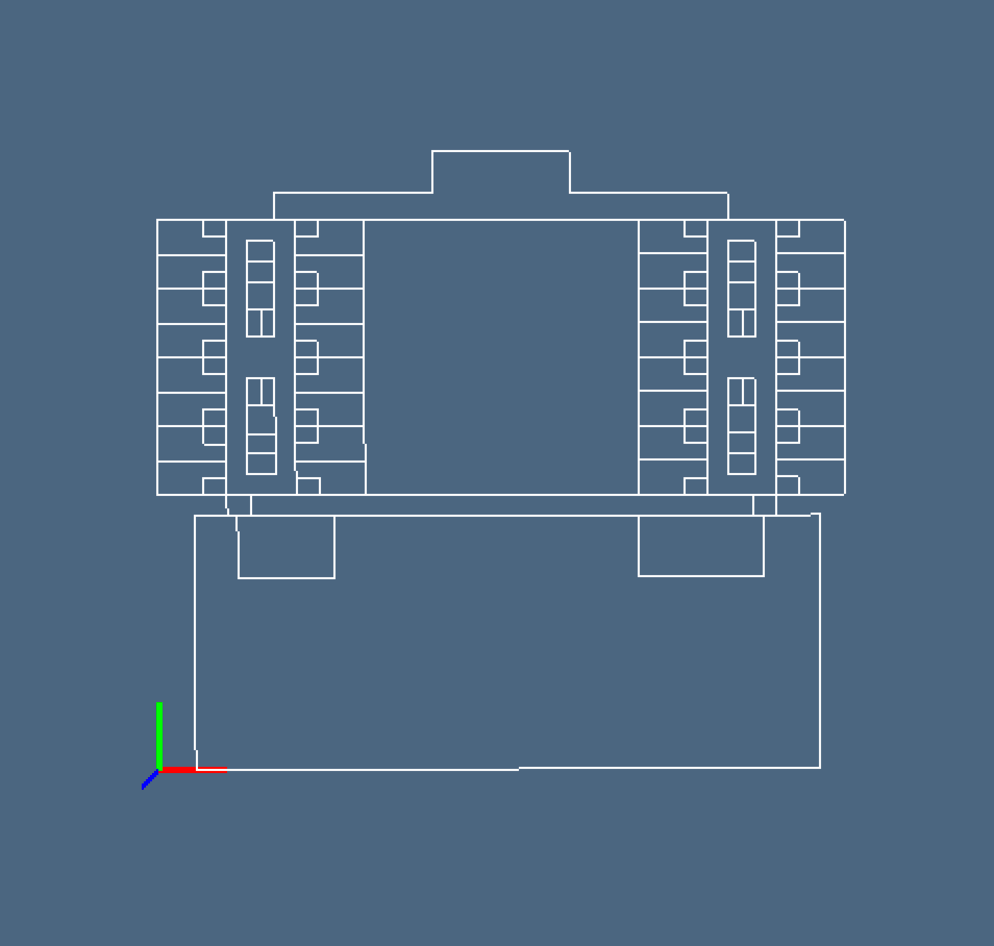
\includegraphics[height=0.329\linewidth,width=0.327\linewidth]{images/secondFloor2} 
   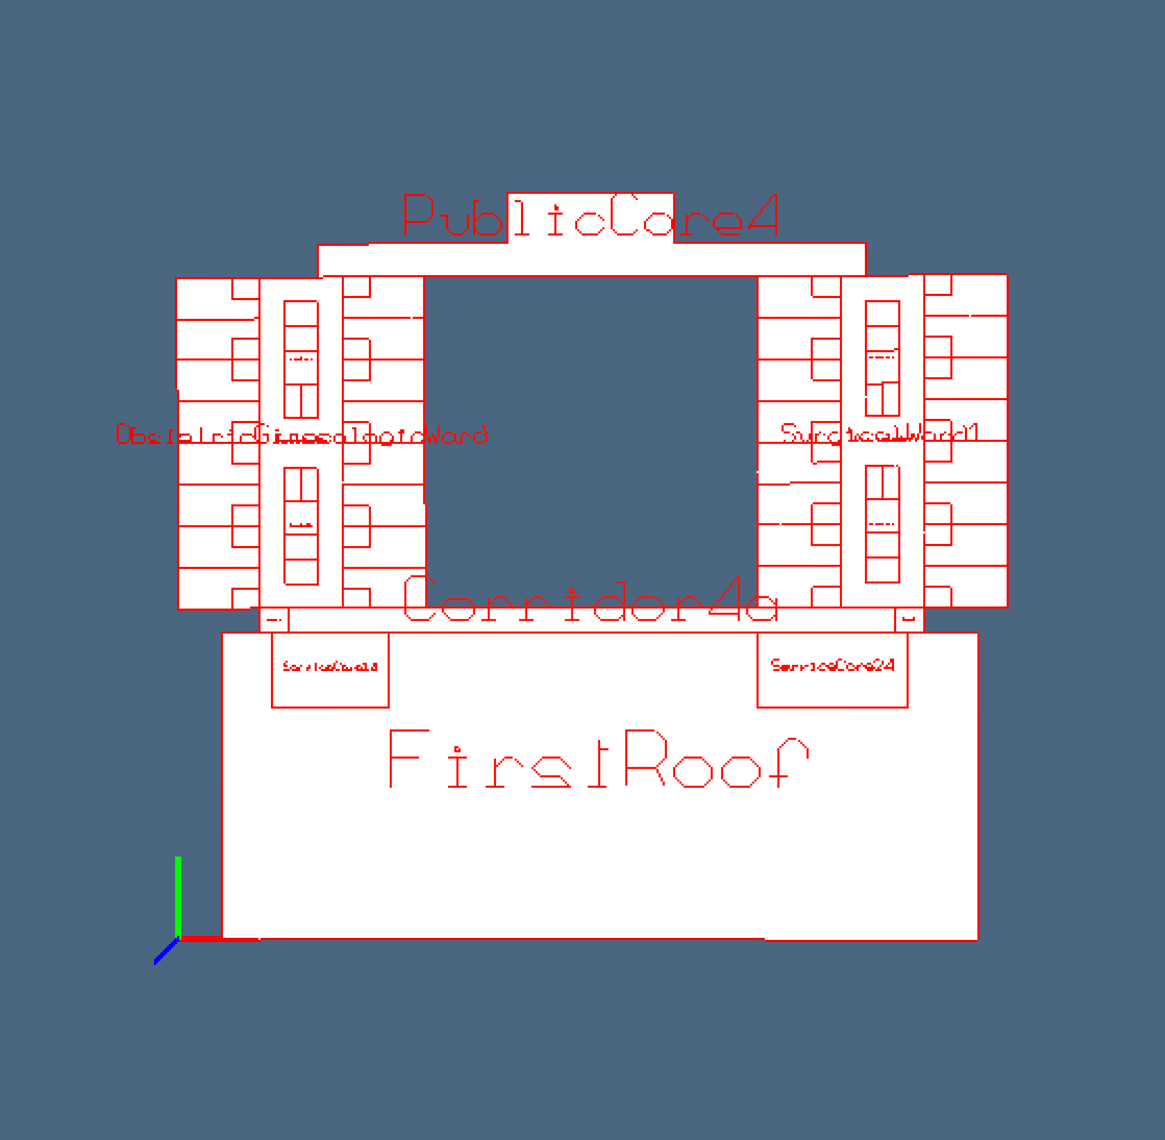
\includegraphics[height=0.329\linewidth,width=0.327\linewidth]{images/secondFloor1} 
   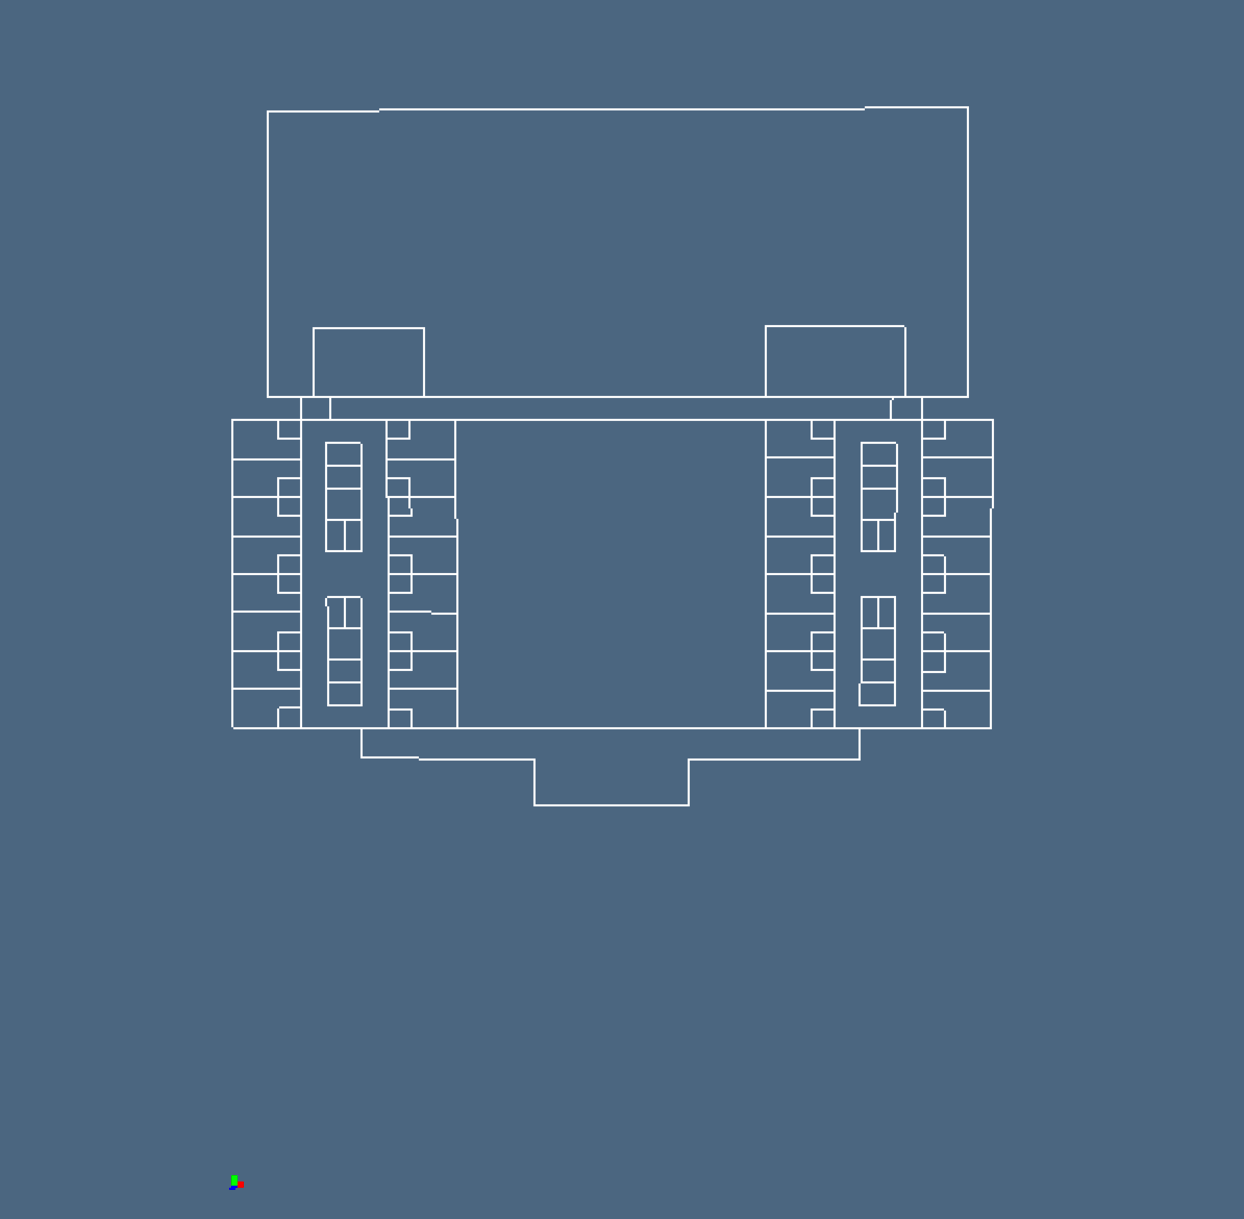
\includegraphics[height=0.329\linewidth,width=0.327\linewidth]{images/secondFloor3} 
   \caption{\texttt{secondFloor} images of (a) the 1-skeleton of its \texttt{LAR} representation, in grid coordinates; (b) component substructures in metric coordinates; (c) 1-skeleton. Notice the position and the scale of the reference frames.}
   \label{fig:secondFloor}
\end{figure}

%-------------------------------------------------------------------------------
@D Second floor structure
@{""" Second floor structure """

@< Second floor's building units @>

buildingUnits3 = [publicCore4,obstetricGinecologicWard,surgicalWard1,filter1,filter2,
serviceCore14,serviceCore24,firstRoof,corridor4a,
corridor4b,corridor4b1,corridor4b2,corridor4c,corridor4c1,corridor4c2]
    
secondFloor = Struct(buildingUnits3, "secondFloor")
@}
%-------------------------------------------------------------------------------



\subsubsection{Third floor}
\paragraph{Third floor}
%-------------------------------------------------------------------------------
@D Third floor
@{""" Third floor floor 
GeneralWard1 = AA(metric)(AA(larTranslate([0,4]))(theWard))
SurgicalWard2 = AA(metric)(AA(larTranslate([7,4]))(theWard)) """
@}
%-------------------------------------------------------------------------------


\paragraph{Third floor's building units}
%-------------------------------------------------------------------------------
@D Third floor's building units 
@{""" Third floor's building units """
ward31 = deepcopy(ward)
ward32 = deepcopy(ward)
generalWard1 = Struct([t(0,4),ward31],'GeneralWard1')
surgicalWard2 = Struct([t(7,4),ward32],'SurgicalWard2')
@}
%-------------------------------------------------------------------------------


\begin{figure}[htbp] %  figure placement: here, top, bottom, or page
   \centering
   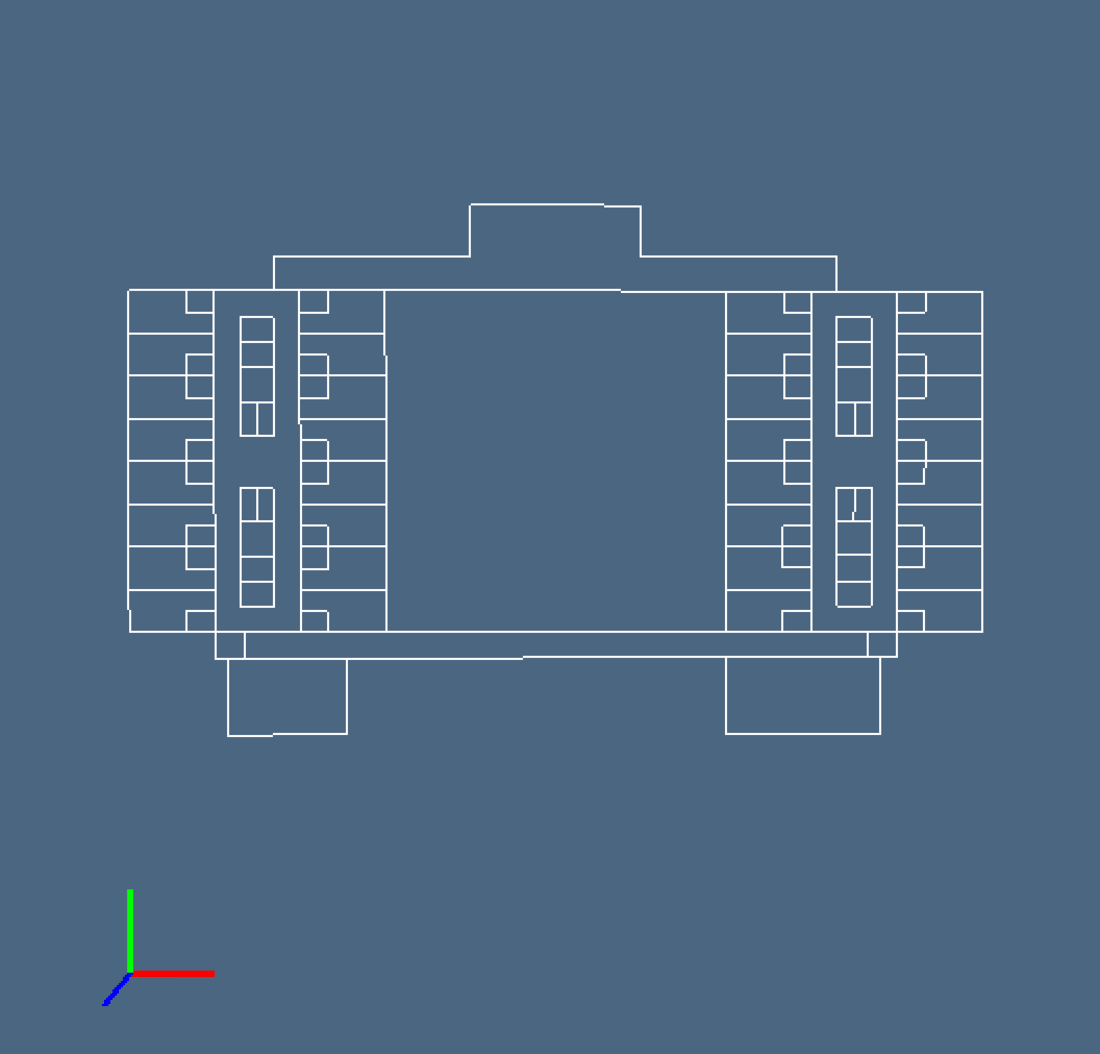
\includegraphics[height=0.329\linewidth,width=0.327\linewidth]{images/thirdFloor2} 
   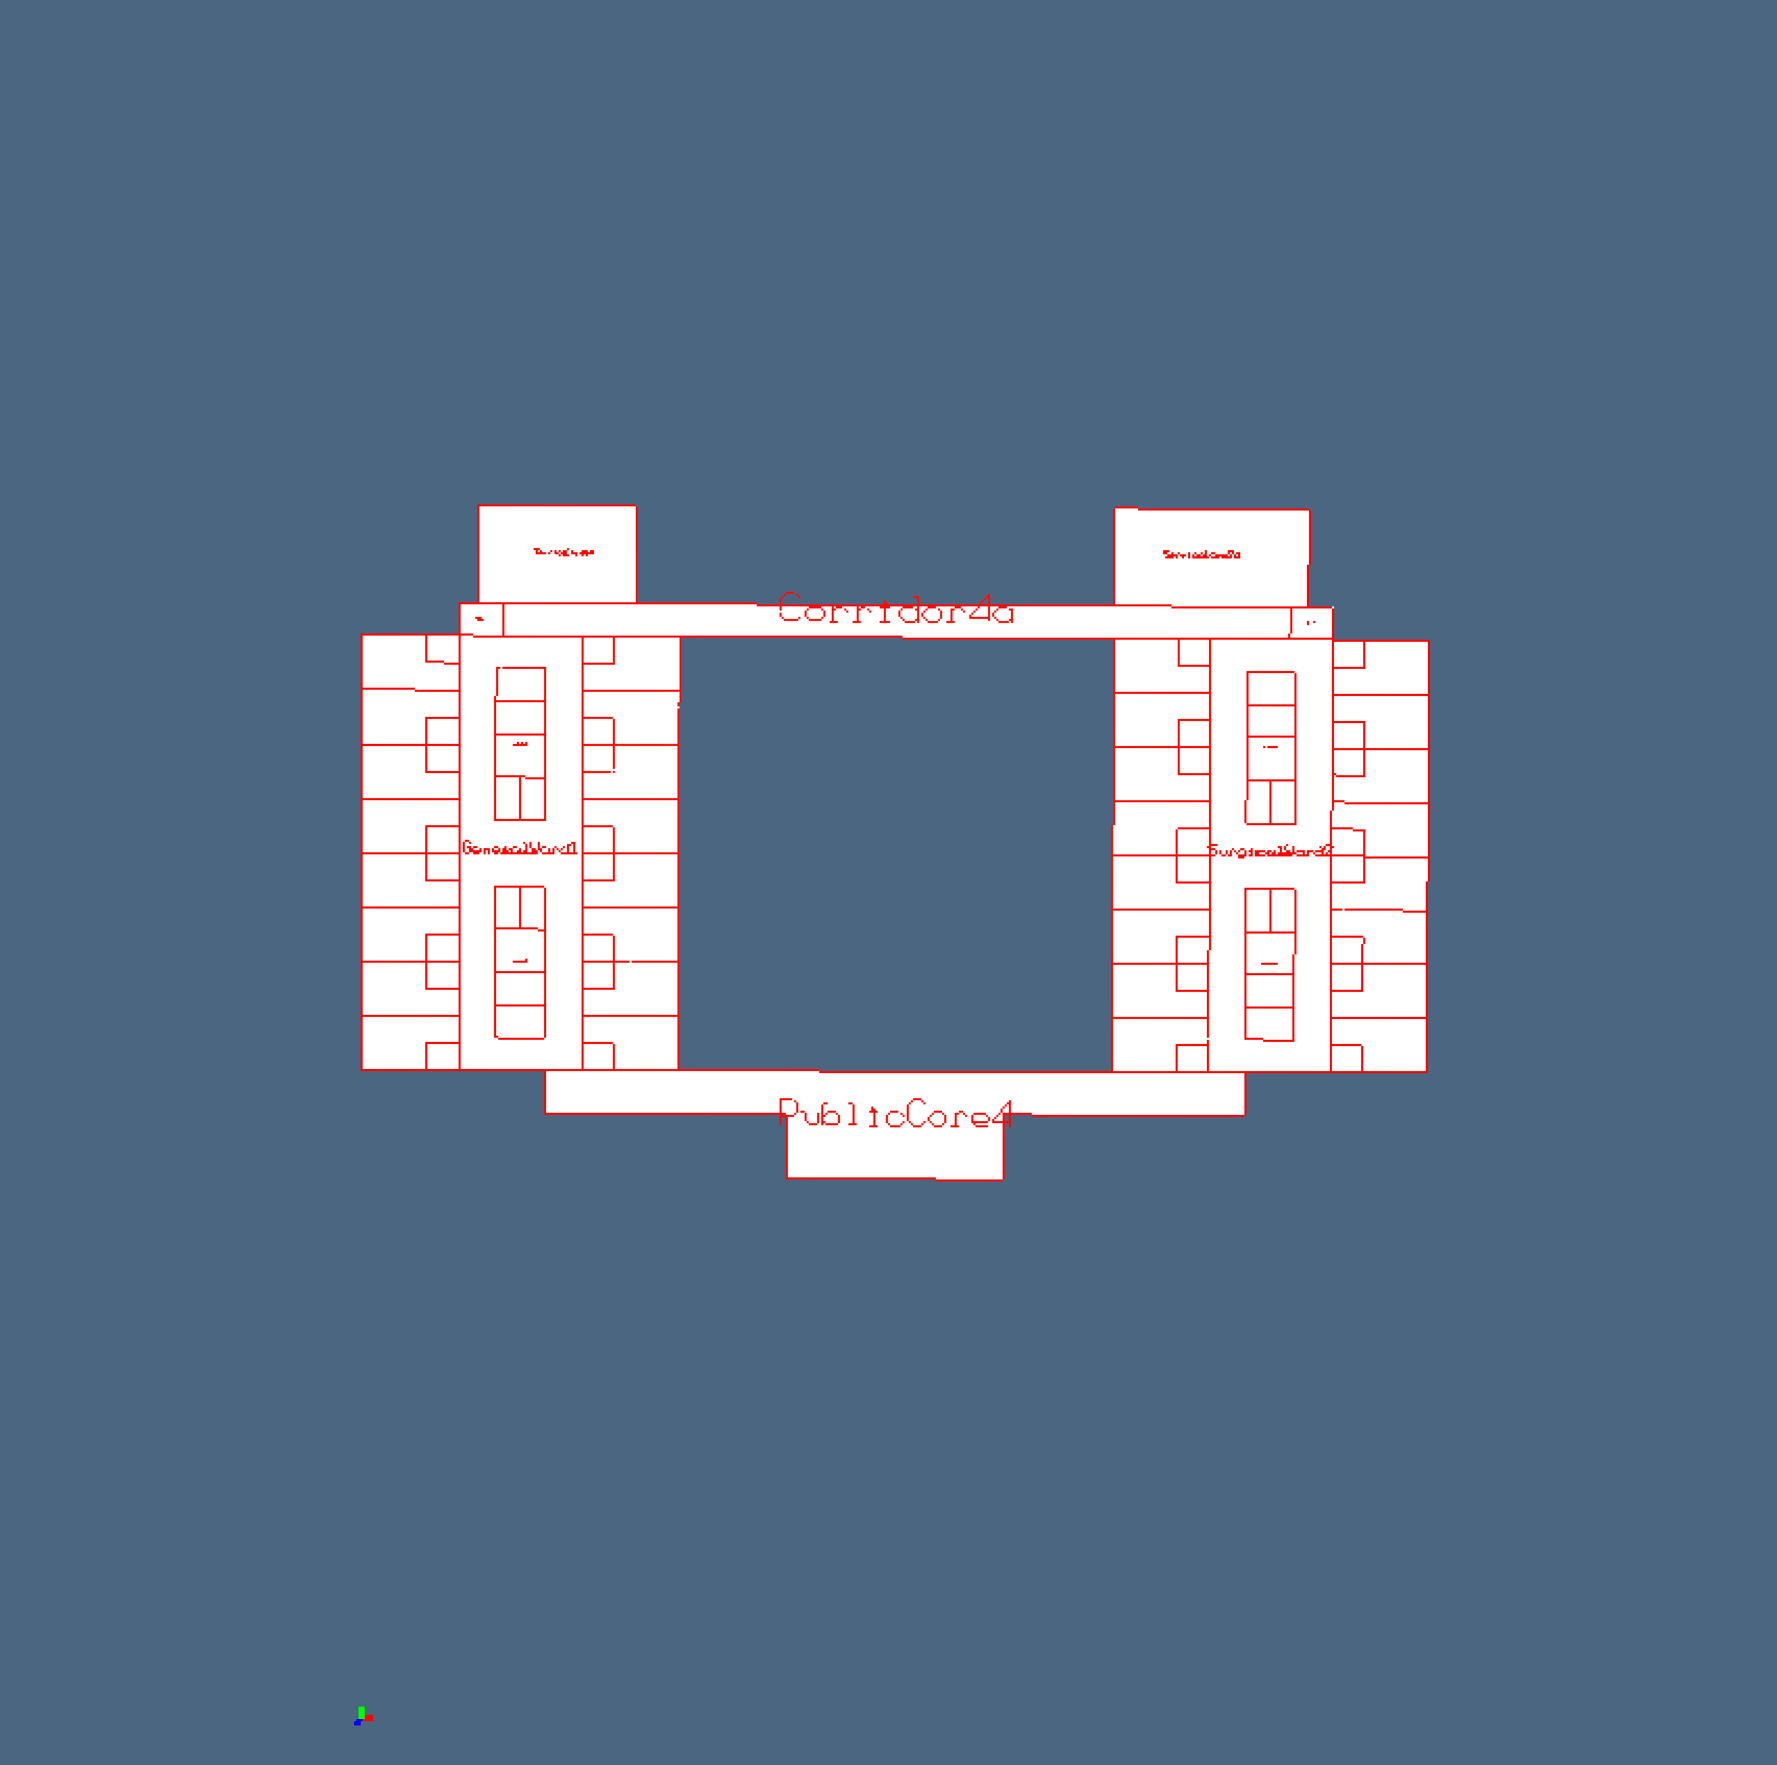
\includegraphics[height=0.329\linewidth,width=0.327\linewidth]{images/thirdFloor1} 
   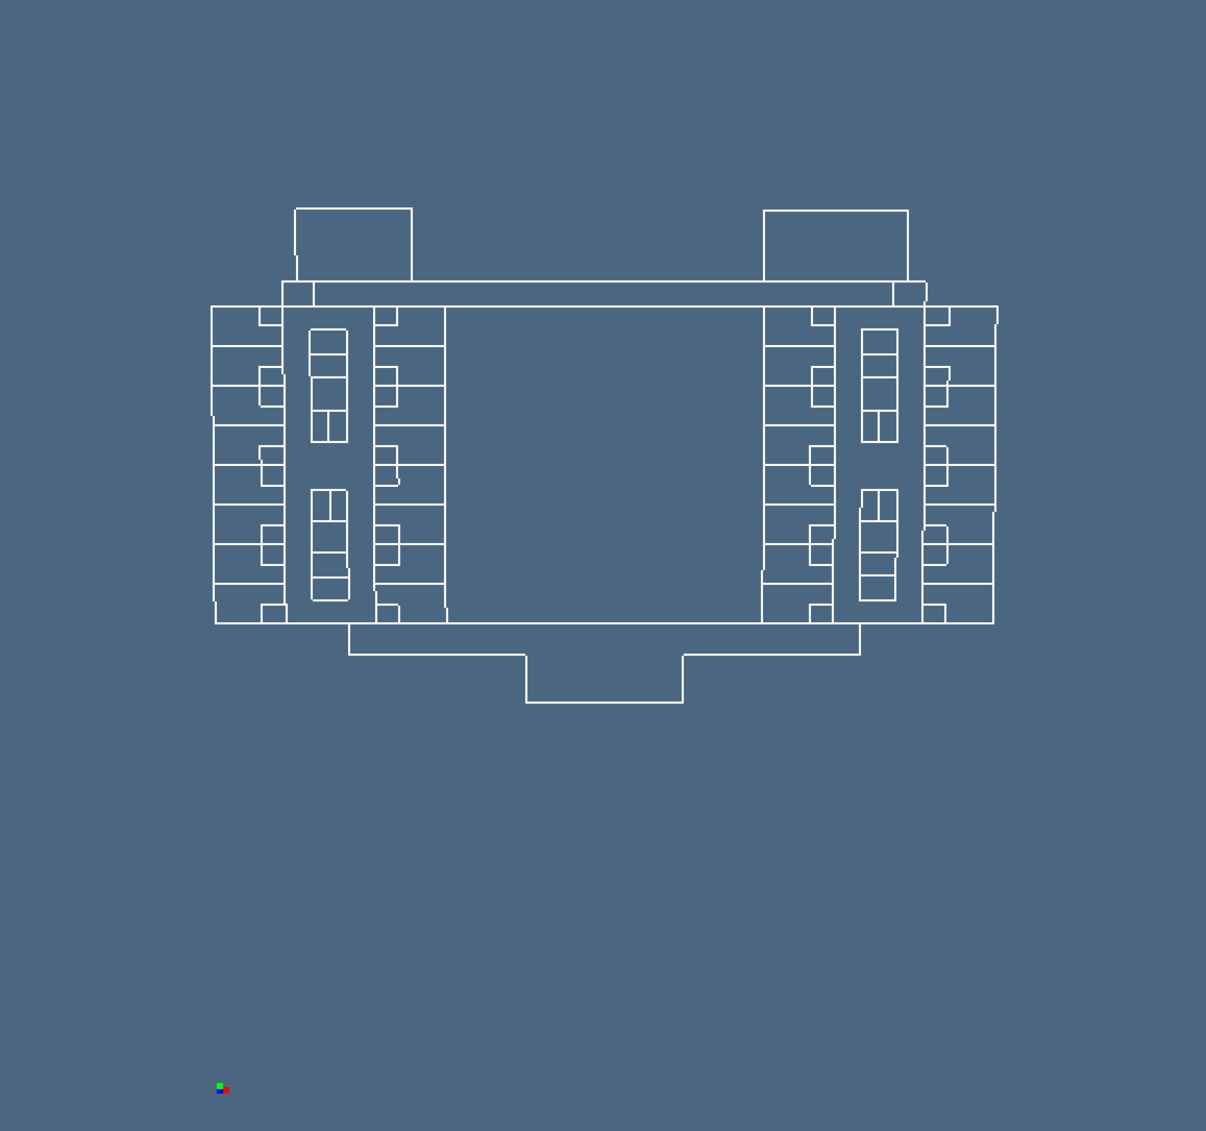
\includegraphics[height=0.329\linewidth,width=0.327\linewidth]{images/thirdFloor3} 
   \caption{\texttt{thirdFloor} images of (a) the 1-skeleton of its \texttt{LAR} representation, in grid coordinates; (b) component substructures in metric coordinates; (c) 1-skeleton. Notice the position and the scale of the reference frames.}
   \label{fig:thirdFloor}
\end{figure}

%-------------------------------------------------------------------------------
@D Third floor structure
@{""" Third floor structure """

@< Third floor's building units @>

buildingUnits4 = [generalWard1,surgicalWard2,publicCore4,serviceCore14,serviceCore24,
                filter1,filter2,corridor4a,corridor4b,corridor4b1,corridor4b2,corridor4c,
                corridor4c1,corridor4c2]

thirdFloor = Struct(buildingUnits4, "thirdFloor")
@}
%-------------------------------------------------------------------------------


\subsubsection{Fourth floor}
\paragraph{Fourth floor}
%-------------------------------------------------------------------------------
@D Fourth floor
@{""" Fourth floor floor 
PediatricWard1 = AA(metric)(AA(larTranslate([0,4]))(theWard))
PediatricWard2 = AA(metric)(AA(larTranslate([7,4]))(theWard)) """
@}
%-------------------------------------------------------------------------------

\paragraph{Fourth floor's building units}
%-------------------------------------------------------------------------------
@D Fourth floor's building units 
@{""" Fourth floor's building units """
ward41 = deepcopy(ward)
ward42 = deepcopy(ward)
pediatricWard1 = Struct([t(0,4),ward41],'PediatricWard1')
pediatricWard2 = Struct([t(7,4),ward42],'PediatricWard2')
@}
%-------------------------------------------------------------------------------

\begin{figure}[htbp] %  figure placement: here, top, bottom, or page
   \centering
   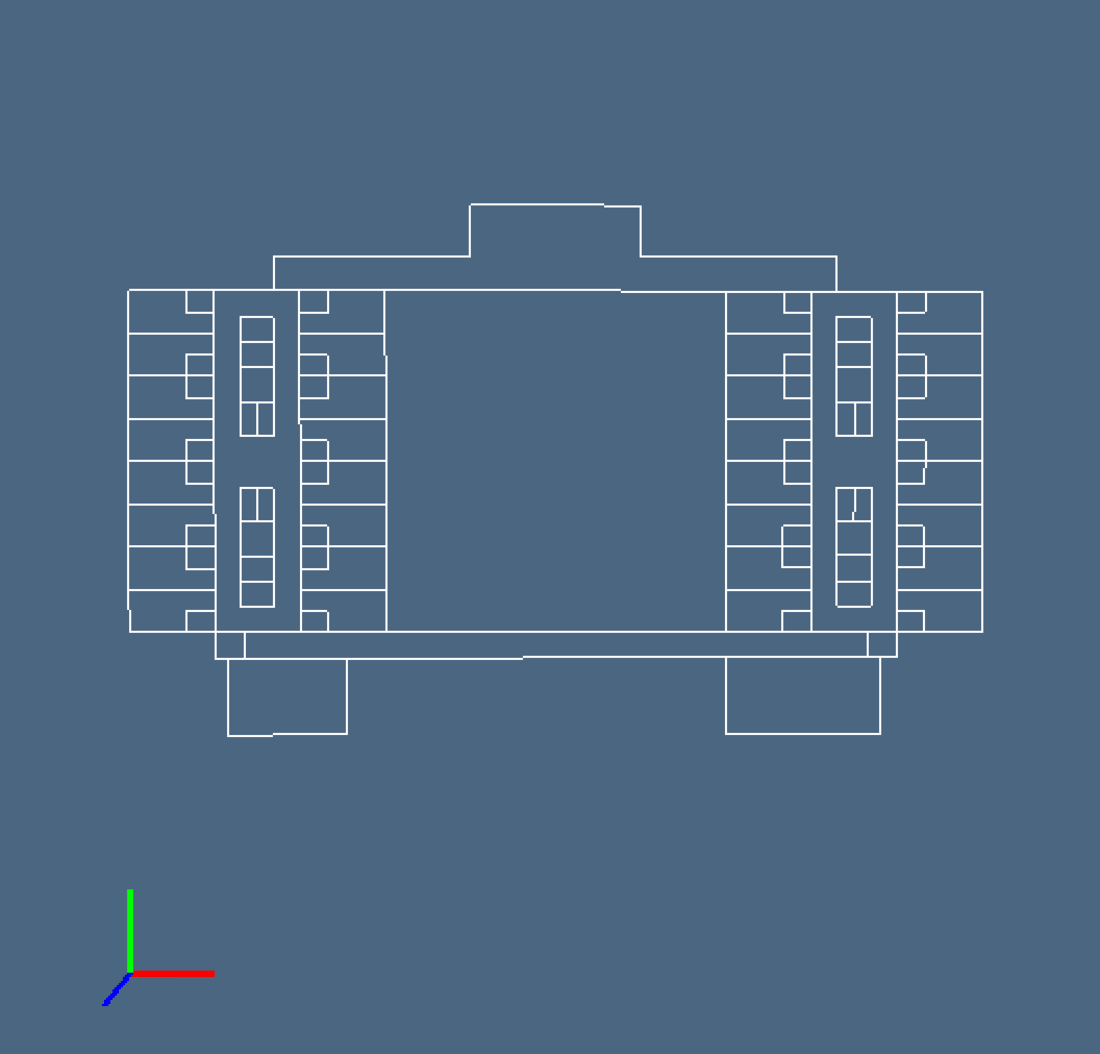
\includegraphics[height=0.329\linewidth,width=0.327\linewidth]{images/thirdFloor2} 
   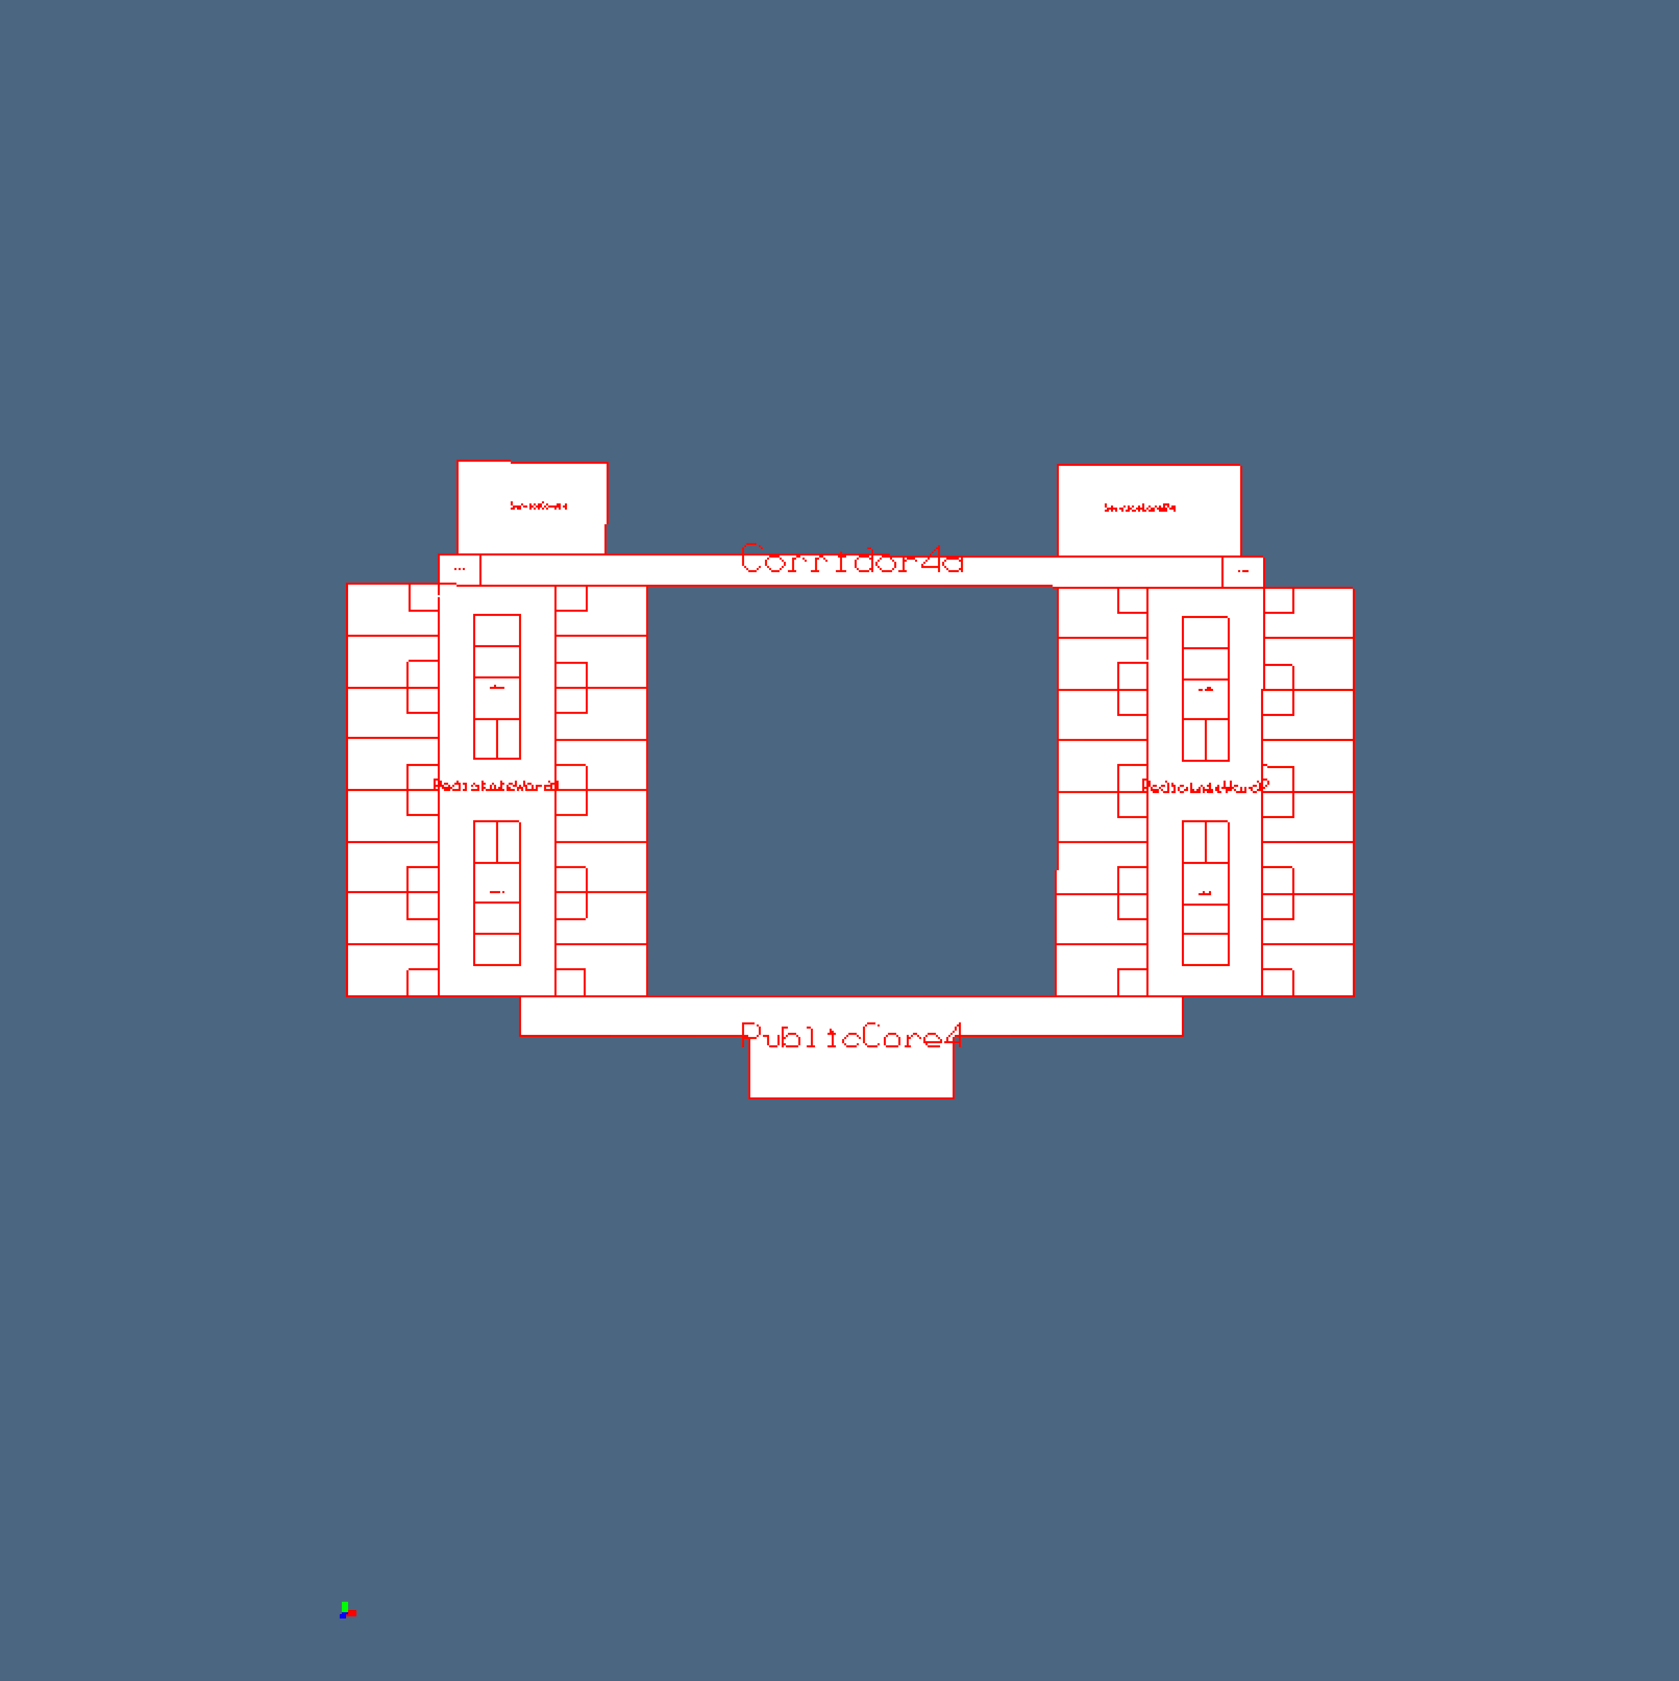
\includegraphics[height=0.329\linewidth,width=0.327\linewidth]{images/fourthFloor1} 
   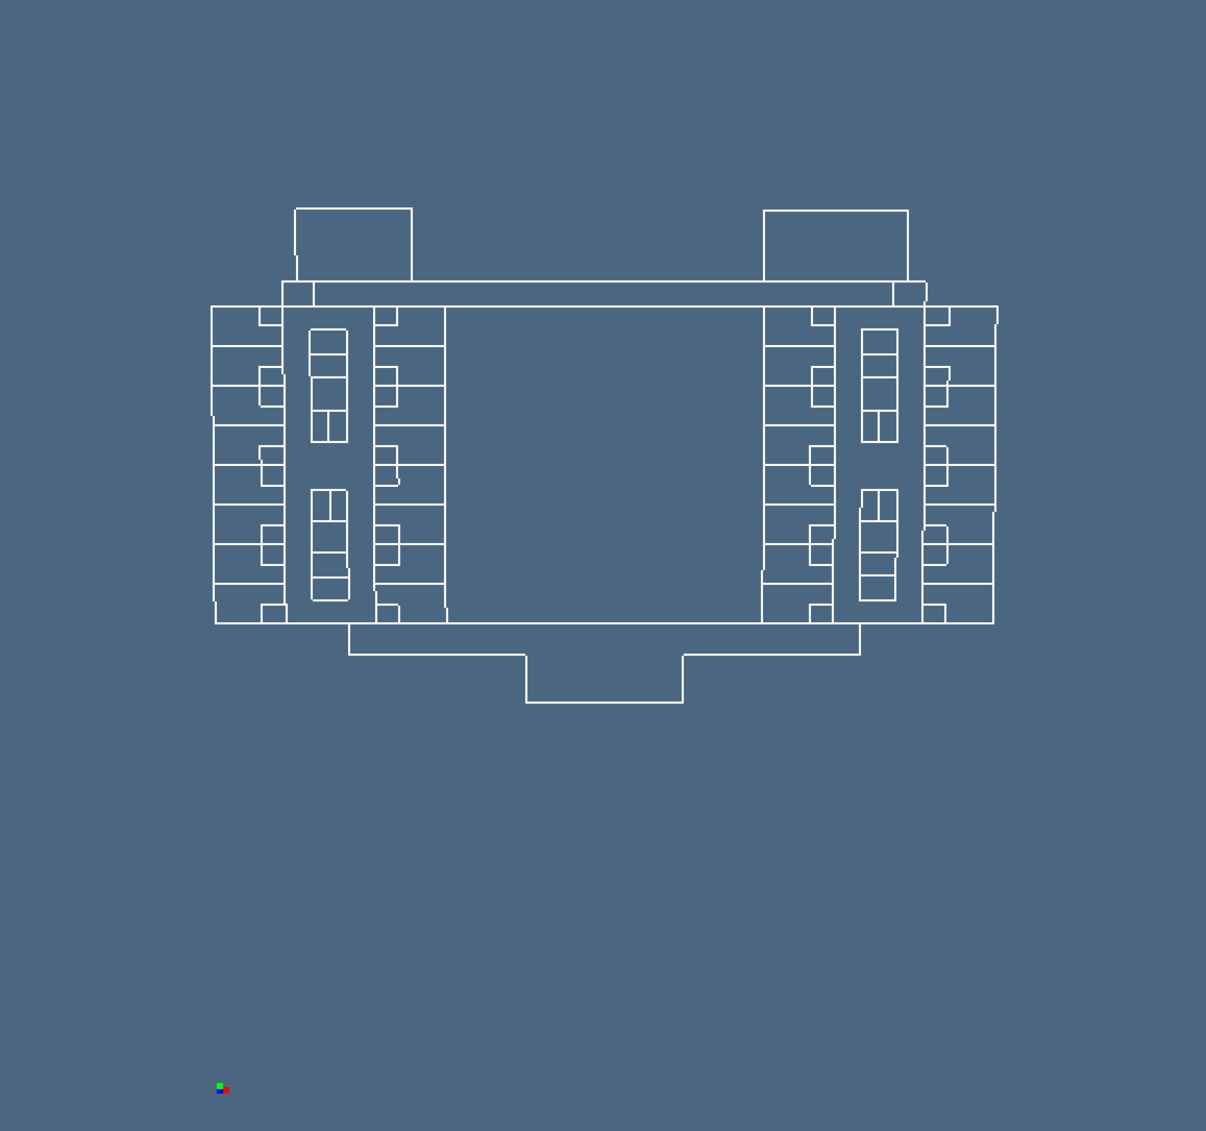
\includegraphics[height=0.329\linewidth,width=0.327\linewidth]{images/thirdFloor3} 
   \caption{\texttt{fourthFloor} images of (a) the 1-skeleton of its \texttt{LAR} representation, in grid coordinates; (b) component substructures in metric coordinates; (c) 1-skeleton. Notice the position and the scale of the reference frames.}
   \label{fig:fourthFloor}
\end{figure}

%-------------------------------------------------------------------------------
@D Fourth floor structure
@{""" Fourth floor structure """

@< Fourth floor's building units @>

buildingUnits5 = [pediatricWard1,pediatricWard2,publicCore4,serviceCore14,serviceCore24,
                filter1,filter2,corridor4a,corridor4b,corridor4b1,corridor4b2,corridor4c,
                corridor4c1,corridor4c2]

fourthFloor = Struct(buildingUnits5, "fourthFloor")
@}
%-------------------------------------------------------------------------------


\subsubsection{Fifth floor}
\paragraph{Fifth floor}
%-------------------------------------------------------------------------------
@D Fifth floor
@{""" Fifth floor floor 
GeneralWard2 = AA(metric)(AA(larTranslate([0,4]))(theWard))
GeneralWard3 = AA(metric)(AA(larTranslate([7,4]))(theWard)) """
@}
%-------------------------------------------------------------------------------


\paragraph{Fifth floor's building units}
%-------------------------------------------------------------------------------
@D Fifth floor's building units 
@{""" Fifth floor's building units """
ward51 = deepcopy(ward)
ward52 = deepcopy(ward)
generalWard2 = Struct([t(0,4),ward51],'GeneralWard2')
generalWard3 = Struct([t(7,4),ward52],'GeneralWard3')
@}
%-------------------------------------------------------------------------------

\begin{figure}[htbp] %  figure placement: here, top, bottom, or page
   \centering
   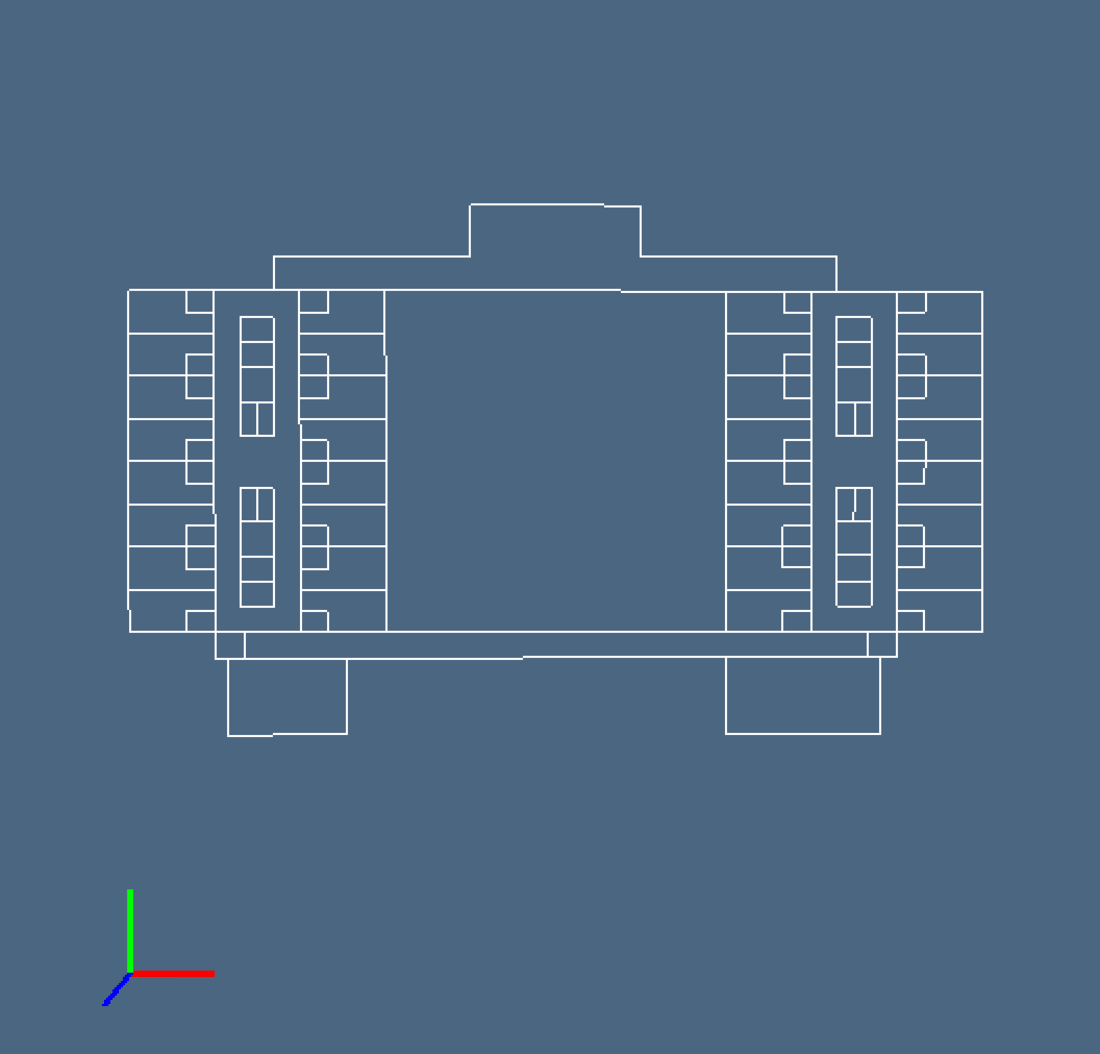
\includegraphics[height=0.329\linewidth,width=0.327\linewidth]{images/thirdFloor2} 
   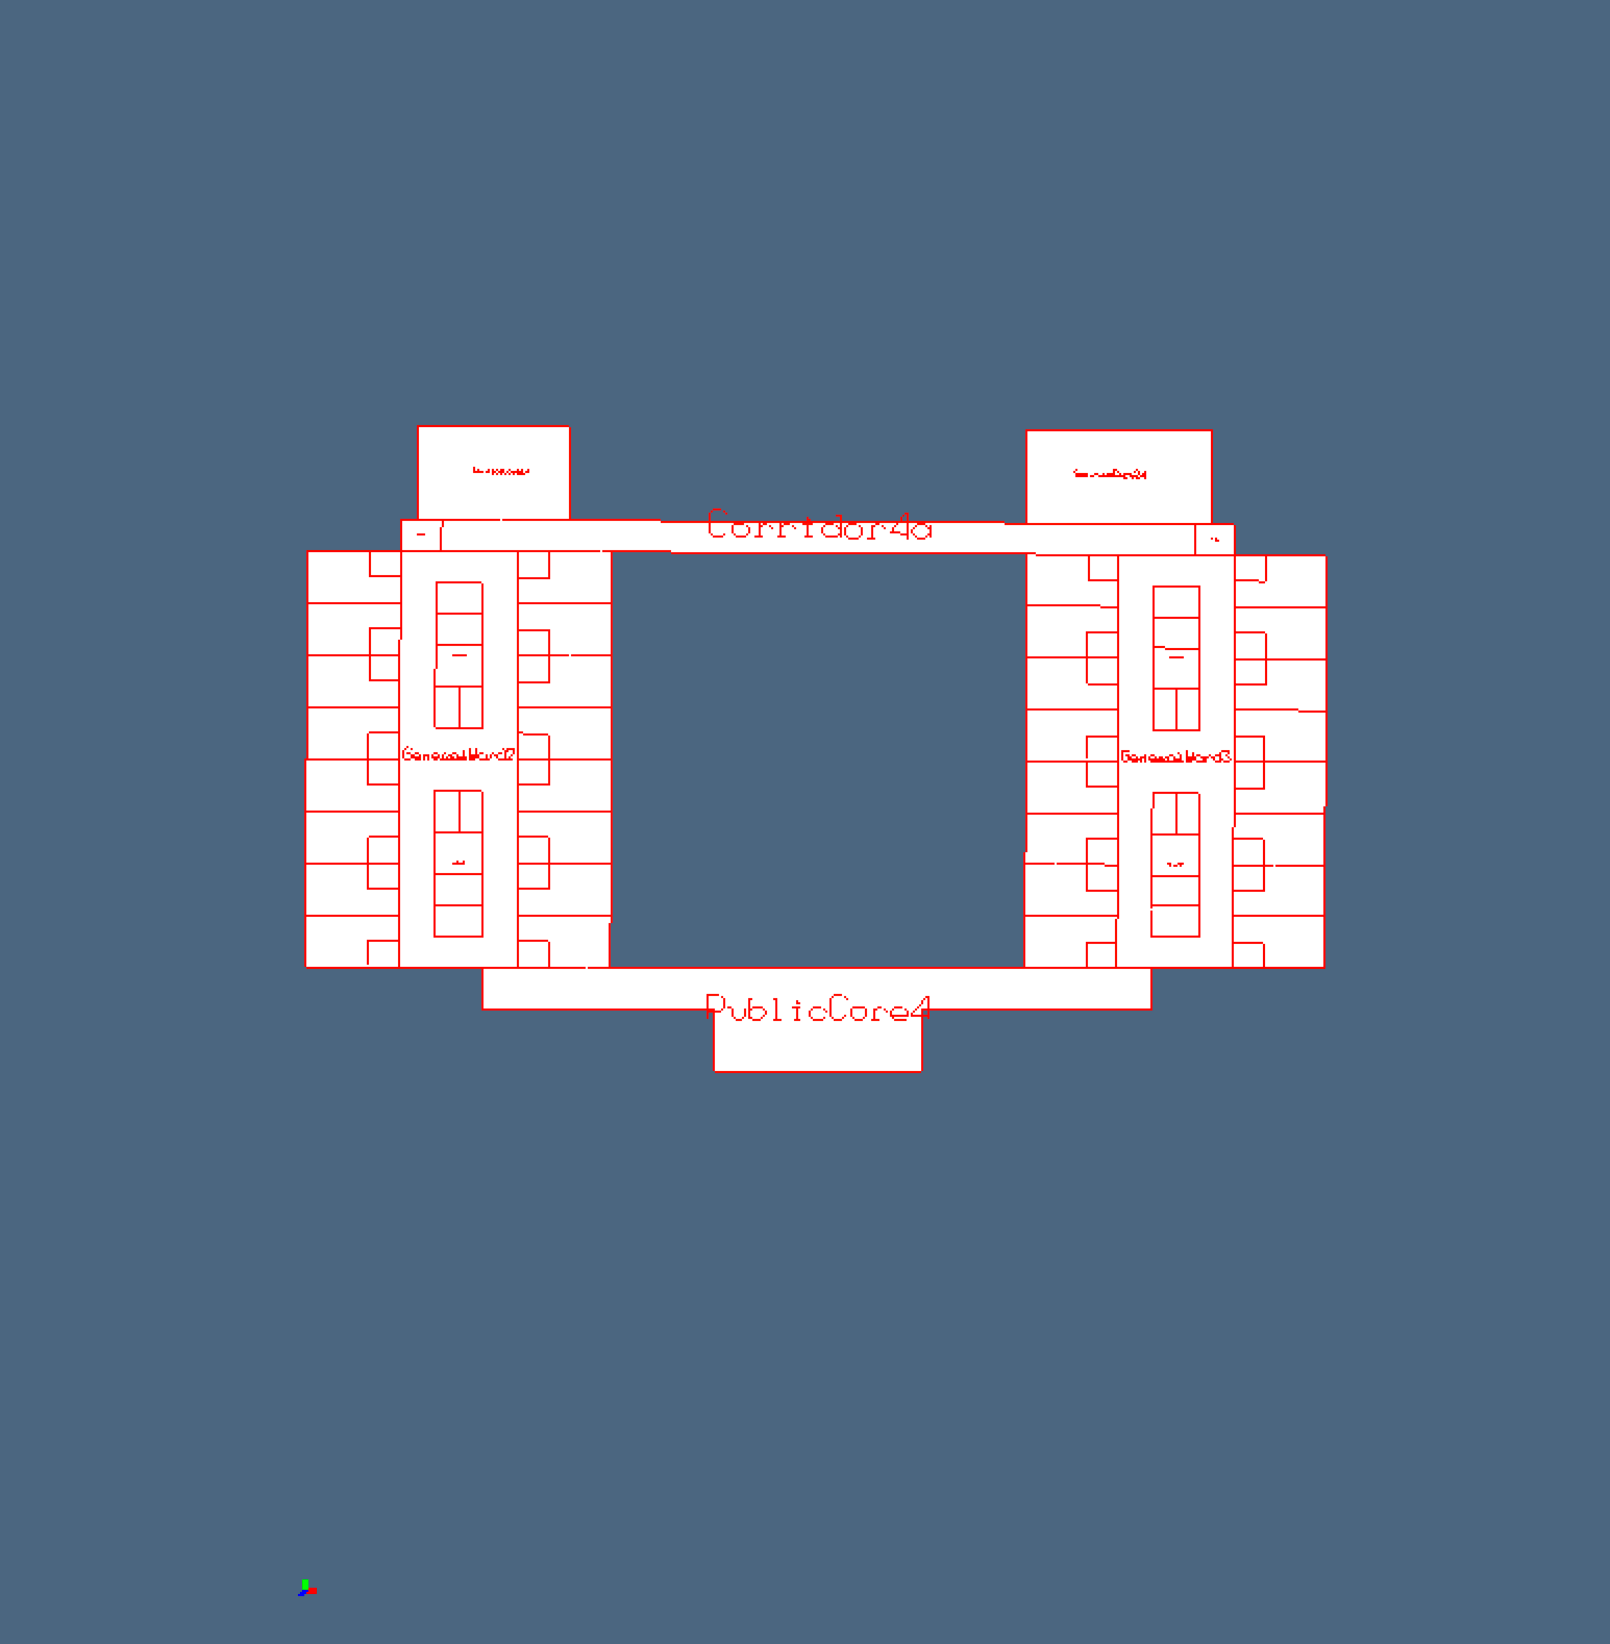
\includegraphics[height=0.329\linewidth,width=0.327\linewidth]{images/fifthFloor1} 
   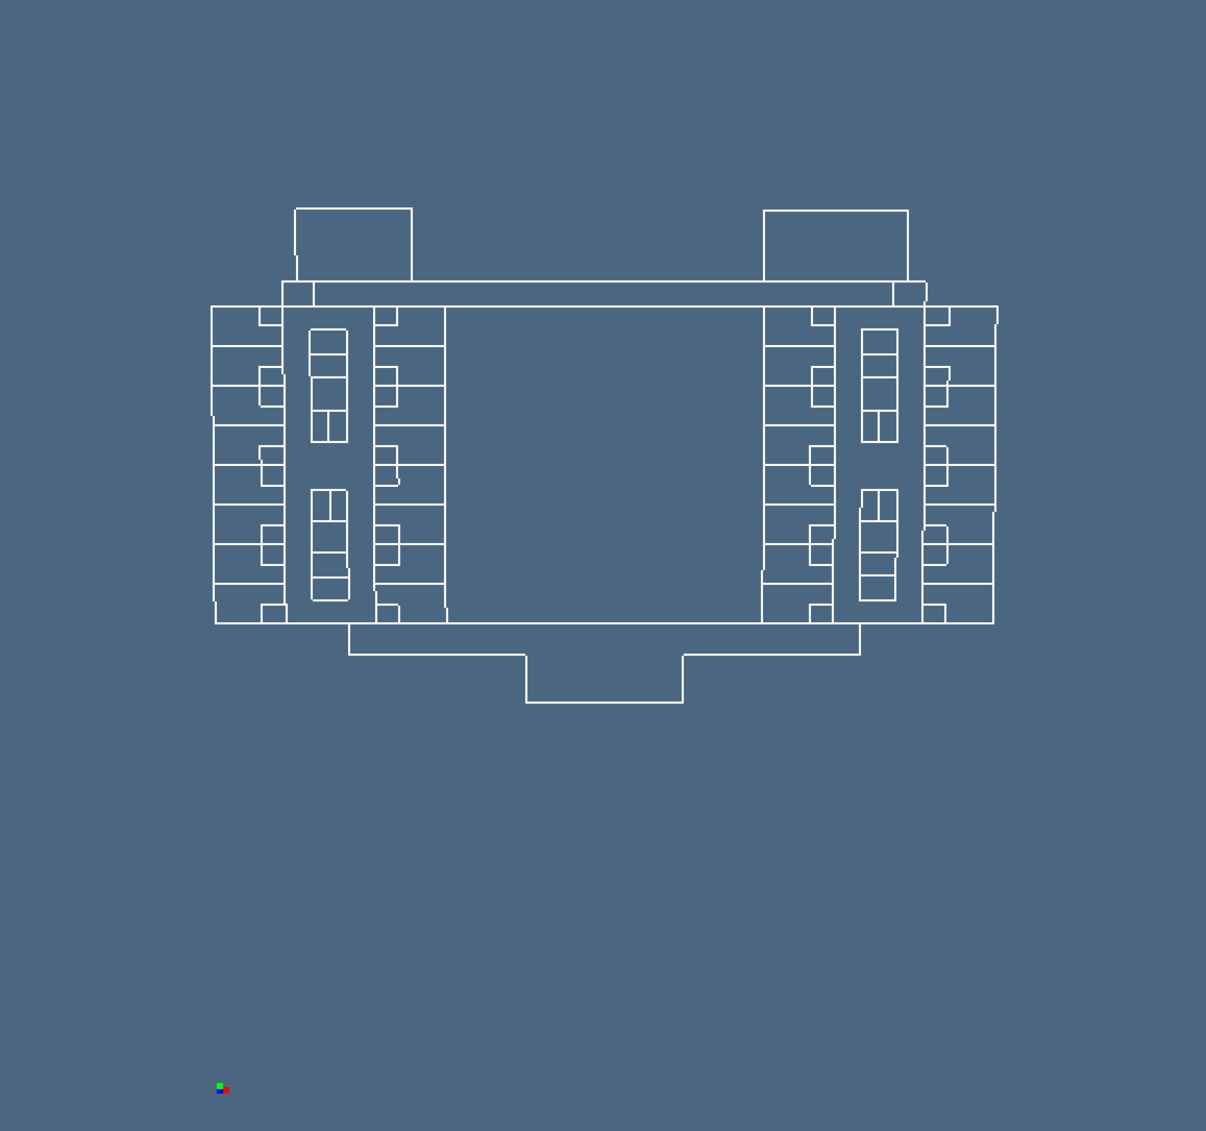
\includegraphics[height=0.329\linewidth,width=0.327\linewidth]{images/thirdFloor3} 
   \caption{\texttt{fifthFloor} images of (a) the 1-skeleton of its \texttt{LAR} representation, in grid coordinates; (b) component substructures in metric coordinates; (c) 1-skeleton. Notice the position and the scale of the reference frames.}
   \label{fig:fifthFloor}
\end{figure}

%-------------------------------------------------------------------------------
@D Fifth floor structure
@{""" Fifth floor structure """

@< Fifth floor's building units @>

buildingUnits6 = [generalWard2,generalWard3,publicCore4,serviceCore14,serviceCore24,
                filter1,filter2,corridor4a,corridor4b,corridor4b1,corridor4b2,
                corridor4c,corridor4c1,corridor4c2]

fifthFloor = Struct(buildingUnits6, "fifthFloor")
@}
%-------------------------------------------------------------------------------



\subsubsection{Storey viewing}

\paragraph{Storey viewing}
%-------------------------------------------------------------------------------
@D Storey generation
@{""" Storey generation """
def structDraw(color,scaling,metric=ID):
    def structDraw0(obj): return obj.draw(color,scaling,metric)
    return structDraw0

if __name__=="__main__":
    
    ground,W,EV = floor(X,Y)(groundFloor,metric)
    ground2D = STRUCT([ground, COLOR(RED)(STRUCT(MKPOLS((W,EV))))] + \
                AA(structDraw(RED,40,metric))(buildingUnits0))
    mezanine,W,EV = floor(X,Y)(mezanineFloor,metric)
    mezanine2D = STRUCT([mezanine, COLOR(RED)(STRUCT(MKPOLS((W,EV))))] + \
                AA(structDraw(RED,40,metric))(buildingUnits1))
    first,W,EV = floor(X,Y)(firstFloor,metric)
    first2D = STRUCT([first, COLOR(RED)(STRUCT(MKPOLS((W,EV))))] + \
                AA(structDraw(RED,40,metric))(buildingUnits2))
    second,W,EV = floor(X,Y)(secondFloor,metric)
    second2D = STRUCT([second, COLOR(RED)(STRUCT(MKPOLS((W,EV))))] + \
                AA(structDraw(RED,40,metric))(buildingUnits3))
    third,W,EV = floor(X,Y)(thirdFloor,metric)
    third2D = STRUCT([third, COLOR(RED)(STRUCT(MKPOLS((W,EV))))] + \
                AA(structDraw(RED,40,metric))(buildingUnits4))
    fourth,W,EV = floor(X,Y)(fourthFloor,metric)
    fourth2D = STRUCT([fourth, COLOR(RED)(STRUCT(MKPOLS((W,EV))))] + \
                AA(structDraw(RED,40,metric))(buildingUnits5))
    fifth,W,EV = floor(X,Y)(fifthFloor,metric)
    fifth2D = STRUCT([fifth, COLOR(RED)(STRUCT(MKPOLS((W,EV))))] + \
                AA(structDraw(RED,40,metric))(buildingUnits6))
@}
%-------------------------------------------------------------------------------

%-------------------------------------------------------------------------------
@D Storey viewing
@{""" Storey viewing """
if __name__=="__main__":
    VIEW(ground2D)
    VIEW(mezanine2D)
    VIEW(first2D)
    VIEW(second2D)
    VIEW(third2D)
    VIEW(fourth2D)
    VIEW(fifth2D)
@}
%-------------------------------------------------------------------------------


\section{Preliminary 2.5D mock-up}

In this section the 2D models of the various hospital floors will be embedded in 3D and translated in the $z$ direction, in order to generate a so-called 2.5D mock-up of the whole building.
This kind of model is often used in the initial planning of complex architectural or engineering designs.

\subsection{Structural frame as cellular complex}

A structural frame is a complex of columns, beams, and trusses connected to one another and to the columns anchored in a foundation, as well as other components or members necessary for the stability of a structure. Floors and roof panels, not connected to the columns (and called secondary members) are not considered part of the structural frame.

While embedding the 2D plans of the architectural design in a common 3D framework, it is important to make explicit choices about the structural frame of the building, that has the major importance in a consistent layout of the various floors. 

From the beginning we noticed that our input hospital model is characterized by a clear and simple structural grid, that can be roughly described as the lattice generated by the Cartesian product of two 1D cellular complexes.


\paragraph{Column locations on grid}

As discussed in Section~\ref{sec:grid}, the reference structural 2D grid is the lattice of integers pairs defined as 
\[
I \times J, \qquad I = [0,14], J = [0,10], \qquad I,J \subset \Z
\]
Only a subset of vertices of this lattice are actually used as pillar positions. A possible way for giving them syntethically is by a collection of sublattices $X_k\times Y_k$ vith extremes $((j_{min},j_{max}),(i_{min},i_{max}))$ such that:
\[
X_k\times Y_k := \texttt{CART([range($j_{min},j_{max}$),range($i_{min},i_{max}$)])}
\]
The subdivision below aims to reconstruct the structural frames at the various floors of the building while assembling all o some of the given subsets.
%-------------------------------------------------------------------------------
@D Column locations on grid @{
""" Column locations on grid """
secondPillars = [((4,5),(1,10)),((3,4),(1,4)),((3,4),(7,10)),((4,8),(0,4)),
    ((4,8),(7,11)),((8,9),(0,11)),((9,10),(4,7))]
firstPillars = [((0,5),(1,10)),((4,8),(0,4)),((4,8),(7,11)),((8,9),(0,11)),
    ((9,10),(4,7))]
frontPillars = [((8,10),(0,11)),((10,11),(0,6)),((10,11),(7,11)),((11,12),
    (0,3)),((11,12),(4,11))]
bottomPillars = [((12,15),(0,5))]
mezaninePillars = firstPillars + frontPillars
pillars = CAT([secondPillars,firstPillars,frontPillars,bottomPillars])

@< Expand column positions @>
@}
%-------------------------------------------------------------------------------
The full expansion of \texttt{pillars} positions, in 2D \emph{grid coordinates}, and corresponding to the ground floor, follows in the script below. Just notice the trick used to remove the possible duplications. A picture of such set of points is given in Figure~\ref{fig:pillars}.
A function \texttt{EXPAND} is given as the \texttt{COMP}osition of a list of functions, to be applied to the \texttt{pillars} data.
%-------------------------------------------------------------------------------
@D Expand column positions  @{
def RANGE(pair): 
    return range(*pair)
EXPAND = COMP([sorted,list,set,AA(tuple),CAT,AA(CART),AA(swap),AA(AA(RANGE))])
@}
%-------------------------------------------------------------------------------

%-------------------------------------------------------------------------------
@D Example of subset of column positions  @{
@< Column locations on grid @>
@< Expand column positions @>

print EXPAND(pillars)

>>> [(0,4),(0,5),(0,6),(0,7),(0,8),(0,9),(0,10),(0,11),(0,12),(0,13),
(0,14),(1,0),(1,1),(1,2),(1,3),(1,4),(1,5),(1,6),(1,7),(1,8),(1,9),
(1,10),(1,11),(1,12),(1,13),(1,14),(2,0),(2,1),(2,2),(2,3),(2,4),
(2,5),(2,6),(2,7),(2,8),(2,9),(2,10),(2,11),(2,12),(2,13),(2,14),
(3,0),(3,1),(3,2),(3,3),(3,4),(3,5),(3,6),(3,7),(3,8),(3,9),(3,10),
(3,12),(3,13),(3,14),(4,0),(4,1),(4,2),(4,3),(4,4),(4,8),(4,9),(4,
10),(4,11),(4,12),(4,13),(4,14),(5,0),(5,1),(5,2),(5,3),(5,4),(5,
8),(5,9),(5,10),(5,11),(6,0),(6,1),(6,2),(6,3),(6,4),(6,8),(6,9),
(6,11),(7,0),(7,1),(7,2),(7,3),(7,4),(7,5),(7,6),(7,7),(7,8),(7,
9),(7,10),(7,11),(8,0),(8,1),(8,2),(8,3),(8,4),(8,5),(8,6),(8,7),
(8,8),(8,9),(8,10),(8,11),(9,0),(9,1),(9,2),(9,3),(9,4),(9,5),(9,
6),(9,7),(9,8),(9,9),(9,10),(9,11),(10,4),(10,5),(10,6),(10,7),
(10,8),(10,9),(10,10),(10,11)]

if __name__=="__main__":
    VIEW(STRUCT(AA(MK)(EXPAND(pillars)))) # grid coordinates
    VIEW(STRUCT(AA(MK)(metric(EXPAND(pillars))))) # metric coordinates
@}
%-------------------------------------------------------------------------------

\begin{figure}[htbp] %  figure placement: here, top, bottom, or page
   \centering
   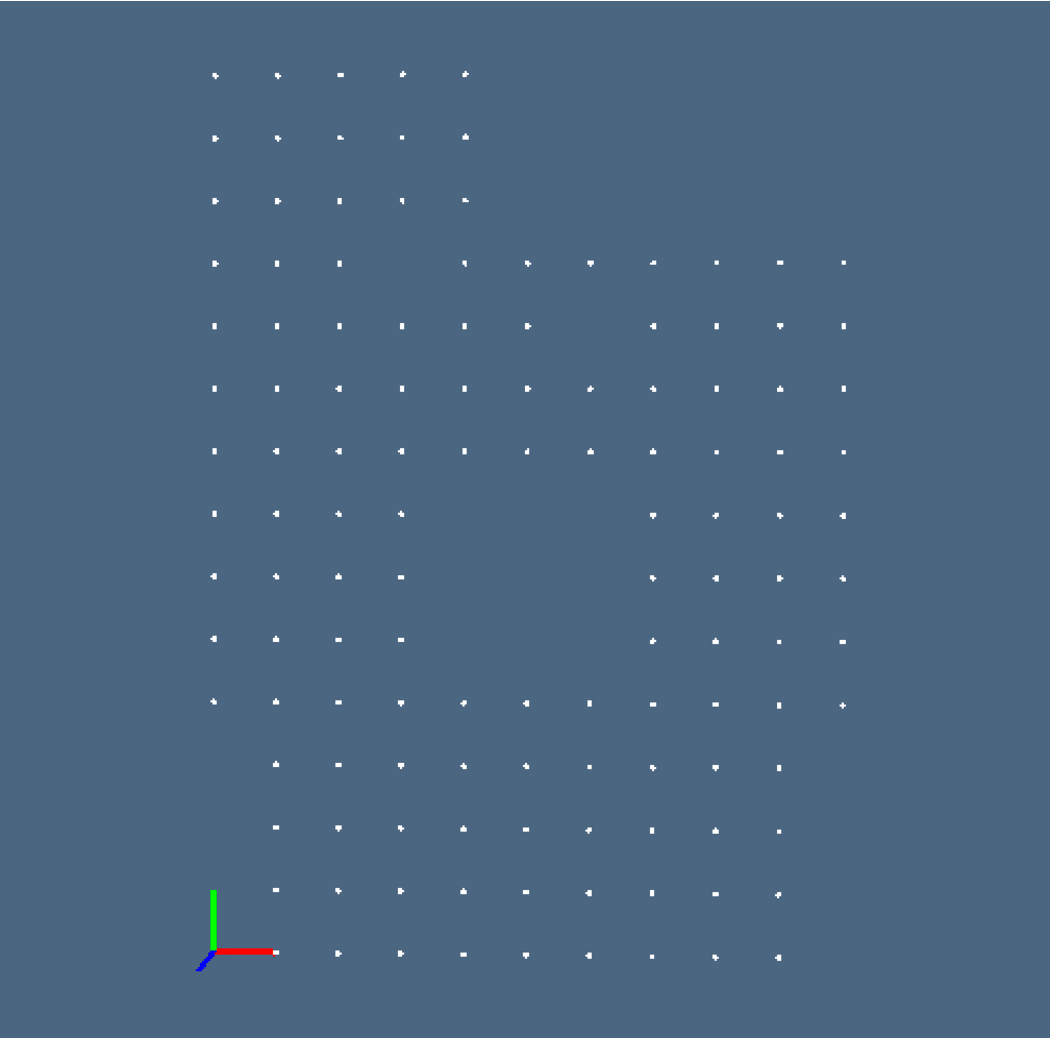
\includegraphics[height=0.33\linewidth,width=0.328\linewidth]{images/pillars1} 
   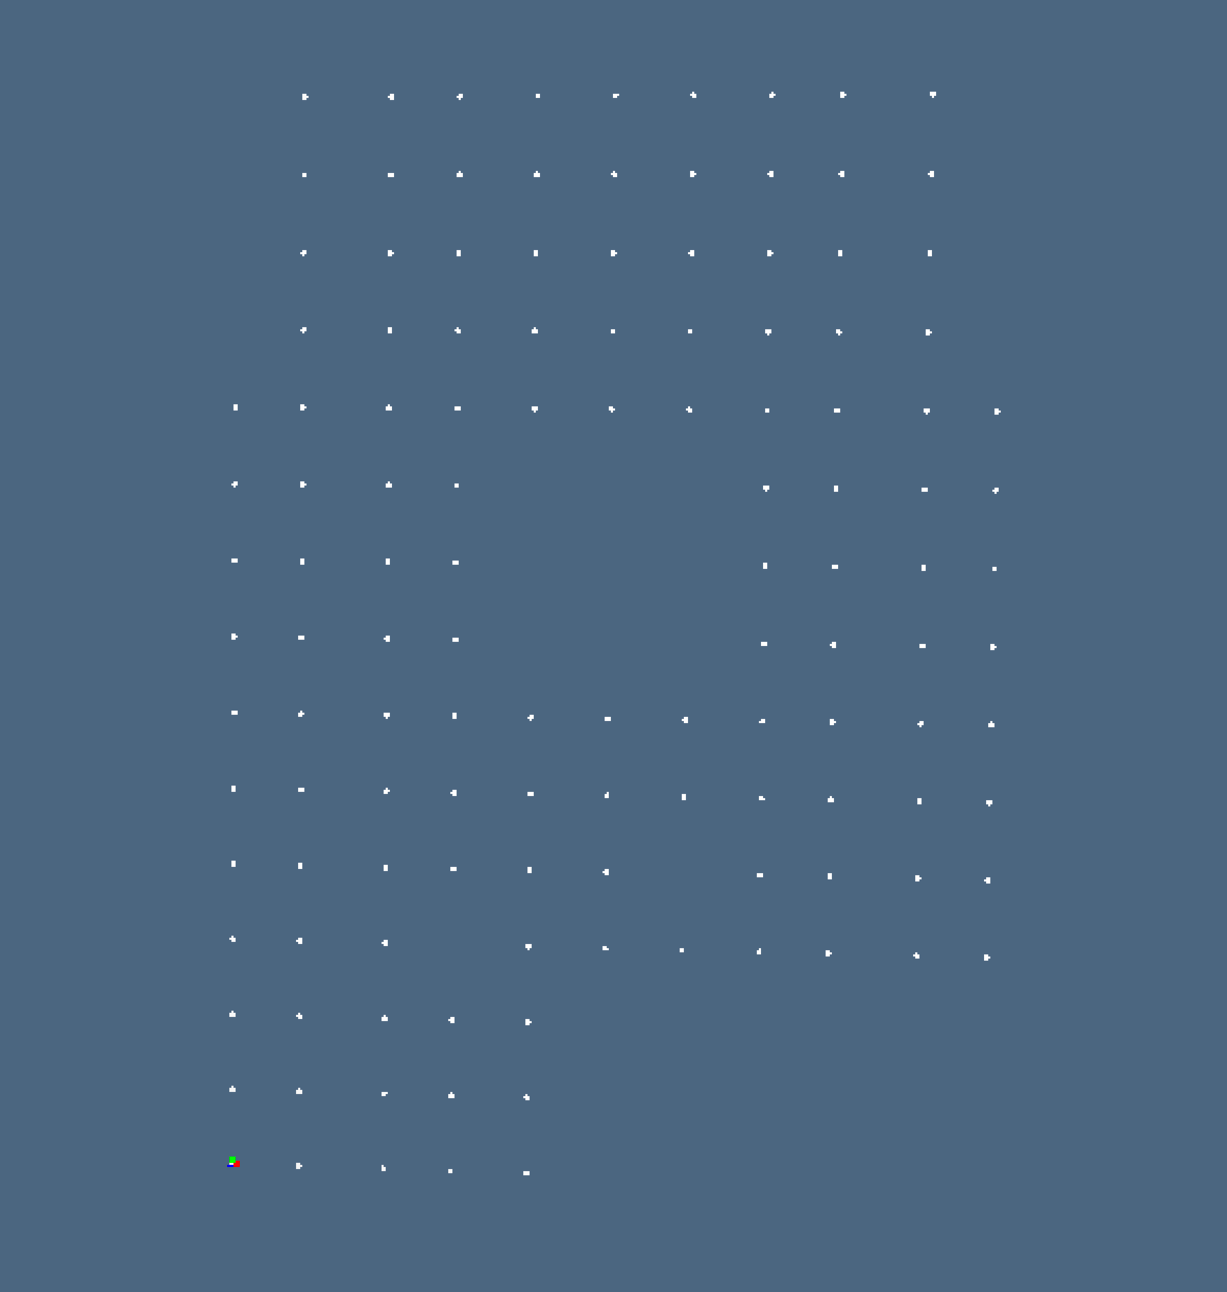
\includegraphics[height=0.33\linewidth,width=0.328\linewidth]{images/pillars2} 
   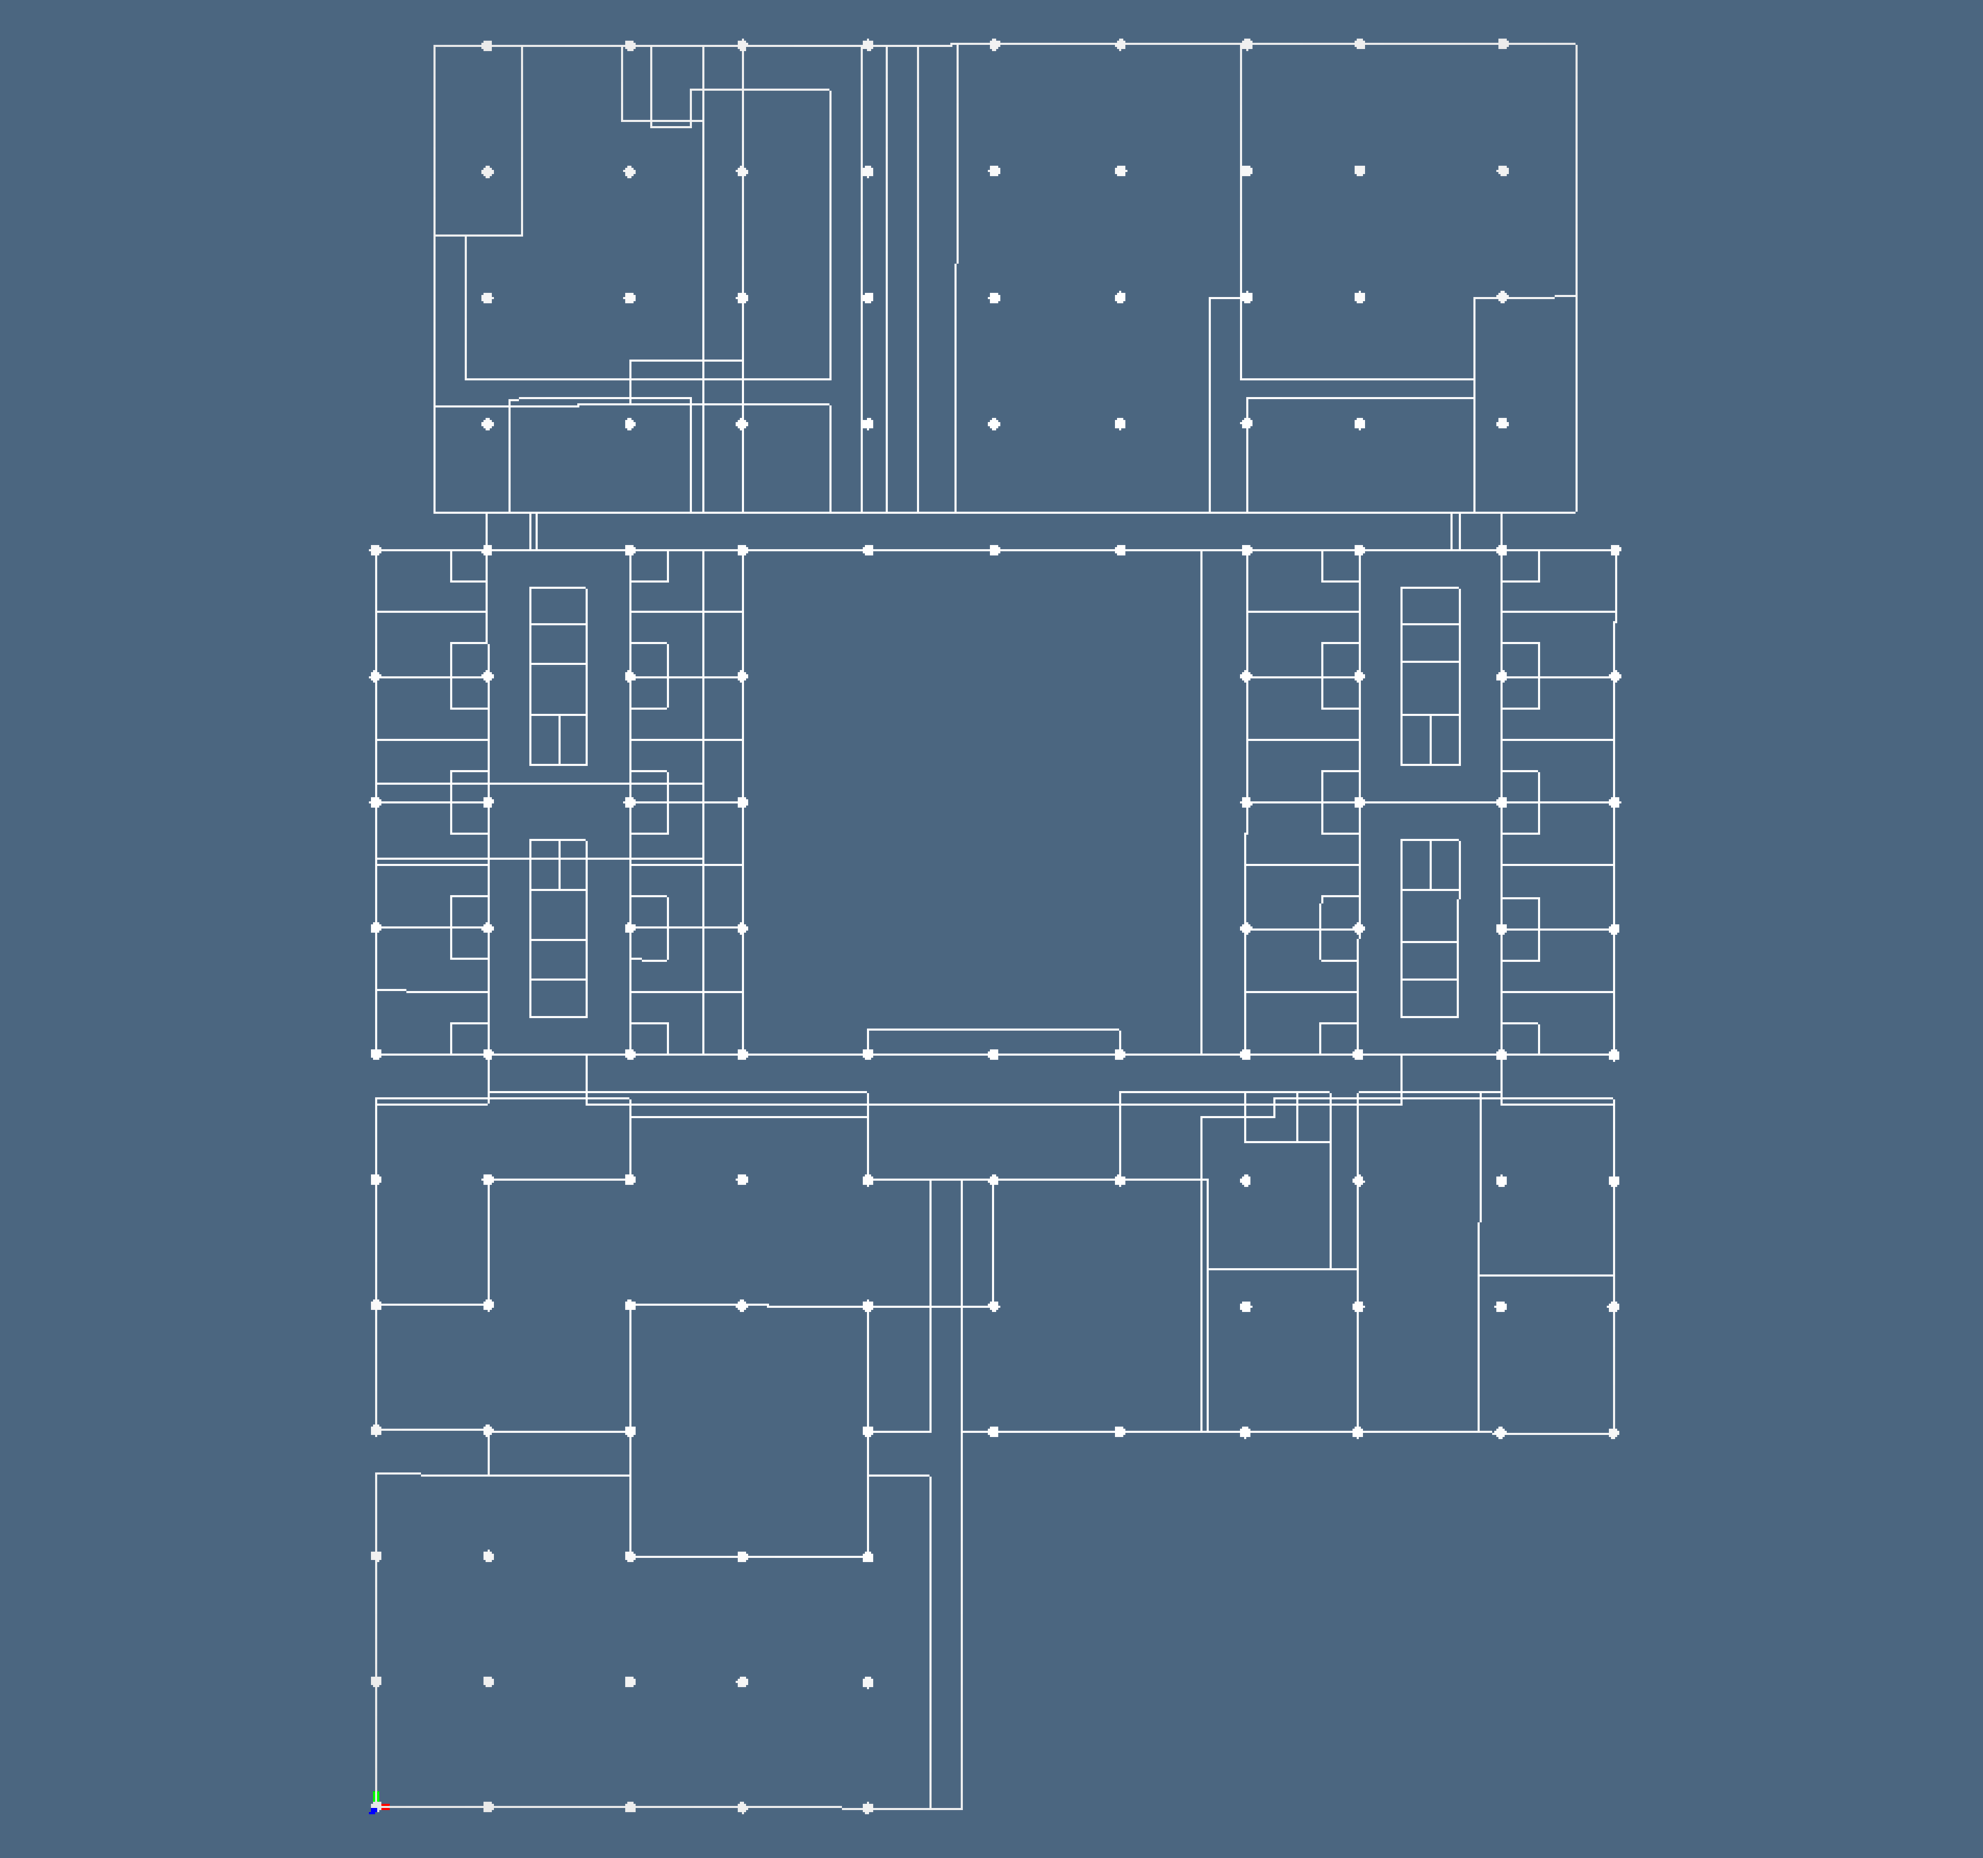
\includegraphics[height=0.33\linewidth,width=0.328\linewidth]{images/pillars3} 
   \caption{The position of pillars of \texttt{groundFloor}, in (a) \emph{grid} and (b) \emph{metric} coordinates, and (c) superimposed to \texttt{floors} layouts.}
   \label{fig:pillars}
\end{figure}

\paragraph{Manhattan test}
The function \texttt{manhattanTest} is used to verify if two nodes of indices \texttt{i},\texttt{j} are either vertically or horizontally adjacent within the set of sublattice points, orderly sorted into the \texttt{nodes} array.
%-------------------------------------------------------------------------------
@D Generation of beams and structural chains 
@{""" Manhattan test """
def manhattanTest(nodes,nDict,i,j):
    hi,ki = nodes[i]
    hj,kj = nodes[j]
    return nDict.setdefault((hi,kj),-1)!=-1 and nDict.setdefault((hj,ki),-1)!=-1
@}
%-------------------------------------------------------------------------------

\paragraph{Generation of beams and structural chains}
%-------------------------------------------------------------------------------
@D Generation of beams and structural chains @{
@< Remove duplicates in structure frame @>

""" Generation of beams and structural chains """
def structureGrid(loci):
    nodes = AA(tuple)(CAT([CART([range(*I), range(*J)]) for (I,J) in loci]))
    nDict = dict([(node,k) for k,node in enumerate(nodes)])
    def node(h,k): return nDict.setdefault((h,k),-1)
    arcs = CAT([[ (node(i,j),node(i,j+1)), (node(i,j),node(i,j-1)),
        (node(i,j),node(i+1,j)), (node(i,j),node(i-1,j)) ] for (i,j) in nodes])
    arcs1 = list(set(AA(tuple)([sorted(arc) for arc in arcs if arc[1]!=-1])))
    arcs = CAT([[ (node(i,j),node(i+1,j+1)), (node(i,j),node(i+1,j-1)),
        (node(i,j),node(i-1,j-1)), (node(i,j),node(i-1,j+1)) ] for (i,j) in nodes])
    arcs2 = list(set(AA(tuple)([sorted(arc) for arc in arcs if arc[1]!=-1])))
    arcs2 = [(i,j) for i,j in arcs2 if manhattanTest(nodes,nDict,i,j)]
    faces = [(node(i,j),node(i,j+1),node(i+1,j+1),node(i+1,j)) for (i,j) in nodes]
    faces = [face for face in faces if not any([v==-1 for v in face])]
    nodes = metric([[j,i] for i,j in nodes])
    return removeDups(nodes,arcs1,arcs2,faces)
@}
%-------------------------------------------------------------------------------


\paragraph{Remove duplicates in structure frame}

For the sake of simplicity and speed, the user's input of sublattice definitions may have non-empty intersections. Therefore, in order to obtain a valid representation of the structural complex, both structural grid vertices and edges must be checked and possible duplicates must be removed. This is achieved by using a Python \emph{defaultdict} data structure \texttt{ndict}, where the indices of duplicated points are accumulated into lists, and then disambiguated using a new numbering of  vertices, codified inside the \texttt{index} array.

%-------------------------------------------------------------------------------
@D Remove duplicates in structure frame 
@{""" Remove duplicates in structure frame """
def removeDups(nodes,arcs1,arcs2,faces):
    ndict = defaultdict(list)
    index = [None for k in range(len(nodes))]
    for k,node in enumerate(nodes):
        ndict[vcode(node)] += [k]
    for h,nodeIndices in enumerate(ndict.values()):
        for k in nodeIndices:
            index[k] = h
    outNodes = [eval(node) for node in ndict.keys()]
    outArcs1 = list(set([tuple(sorted([index[i],index[j]])) for i,j in arcs1]))
    outArcs2 = list(set([tuple(sorted([index[i],index[j]])) for i,j in arcs2]))
    outFaces = list(set([tuple(sorted([index[i],index[j],index[h],index[k]])) 
        for i,j,h,k in faces]))
    return outNodes, outArcs1,outArcs2,outFaces
@}
%-------------------------------------------------------------------------------

\begin{figure}[htbp] %  figure placement: here, top, bottom, or page
   \centering
   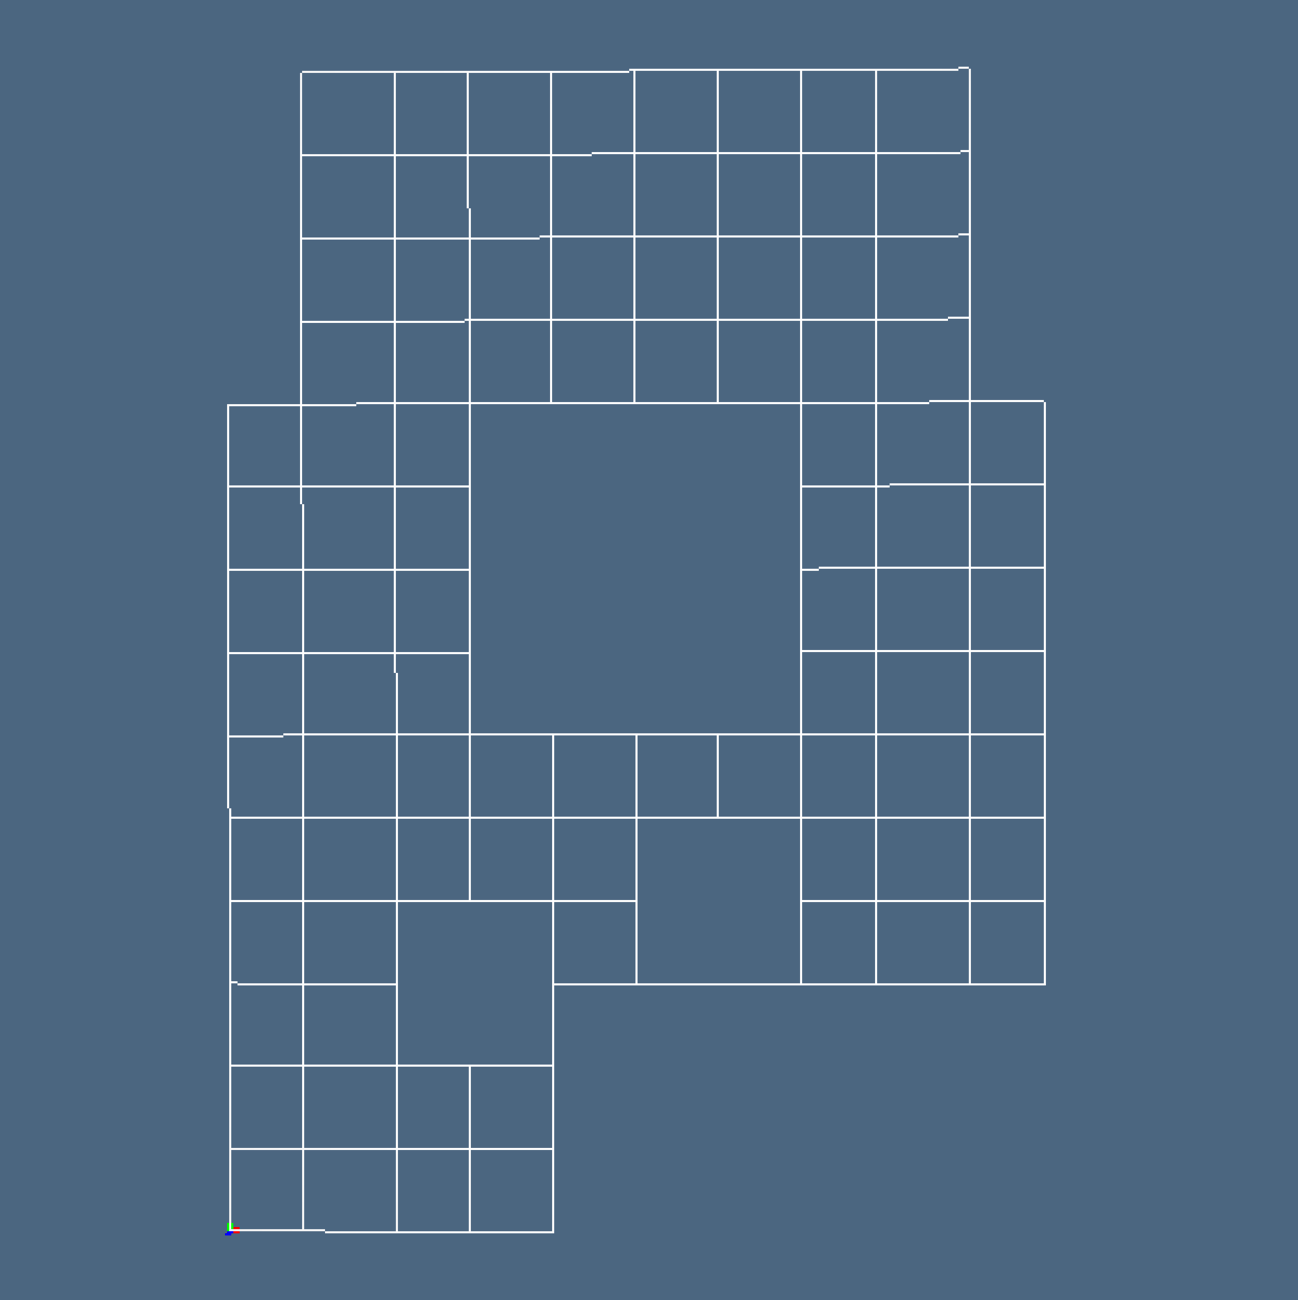
\includegraphics[height=0.243\linewidth,width=0.243\linewidth]{images/frame1} 
   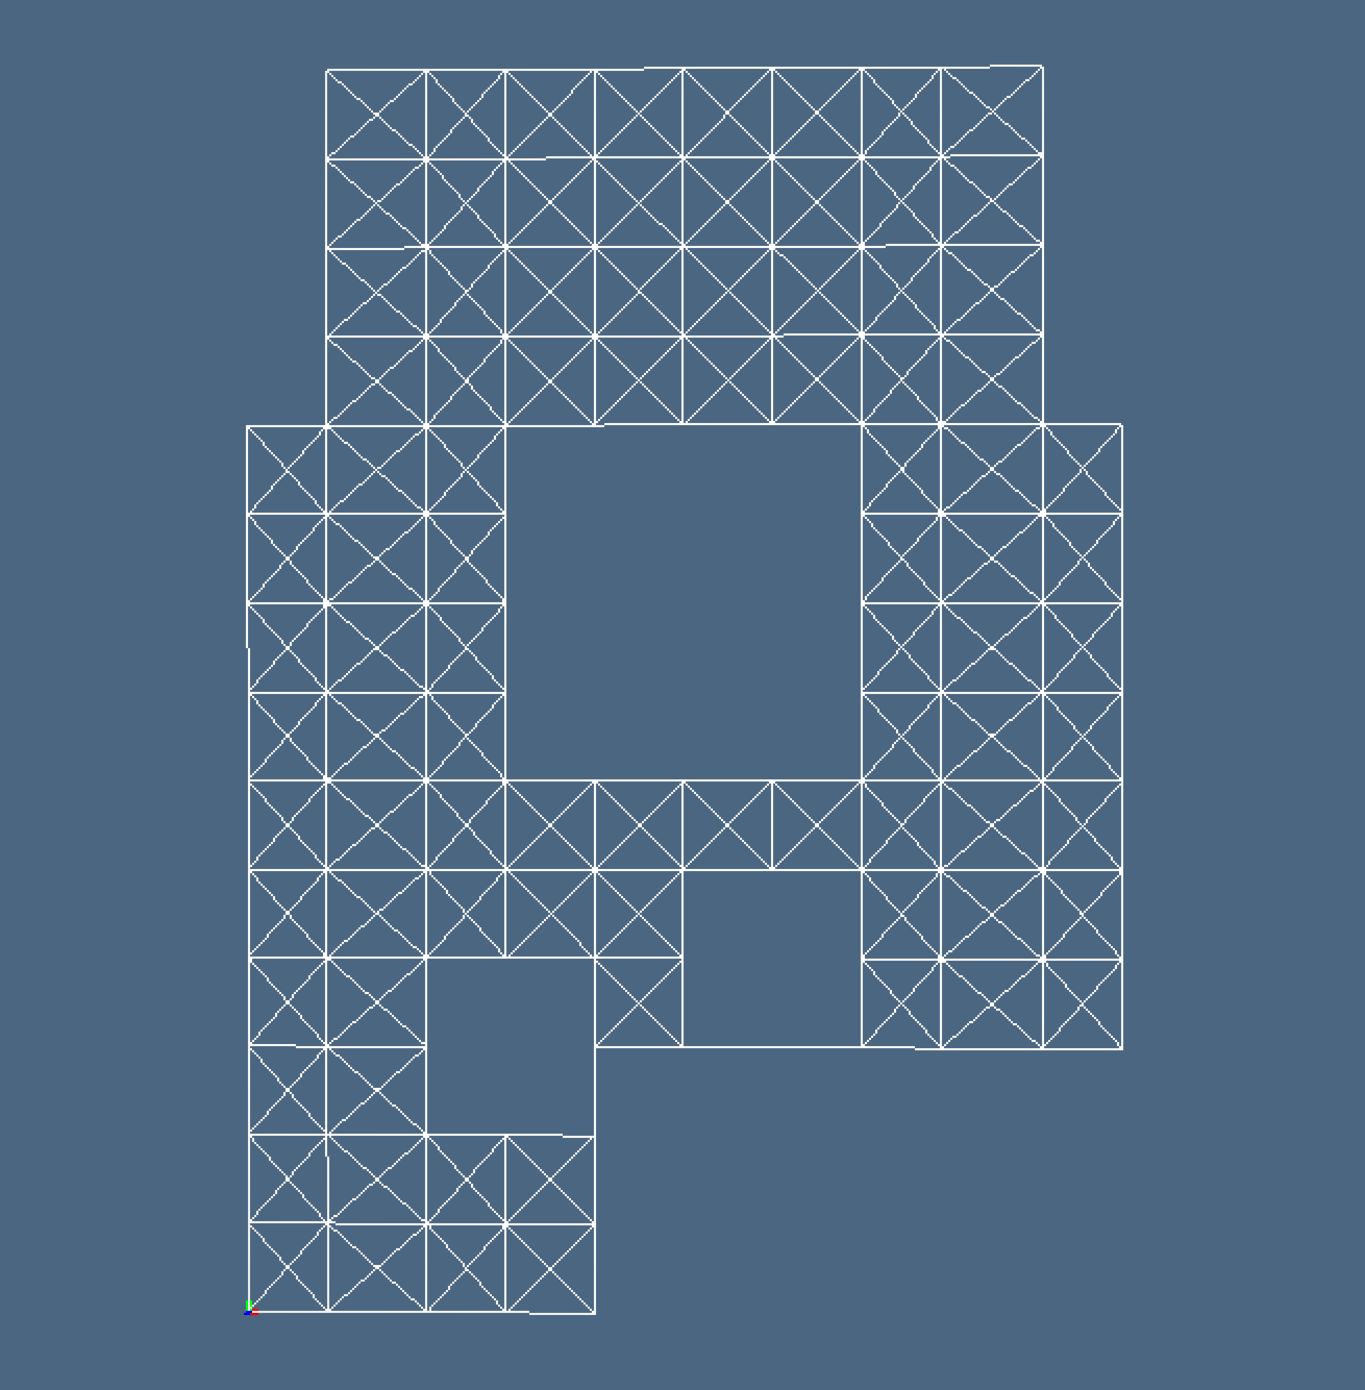
\includegraphics[height=0.243\linewidth,width=0.243\linewidth]{images/frame2} 
   
\includegraphics[height=0.243\linewidth,width=0.243\linewidth]{images/frame3} 
   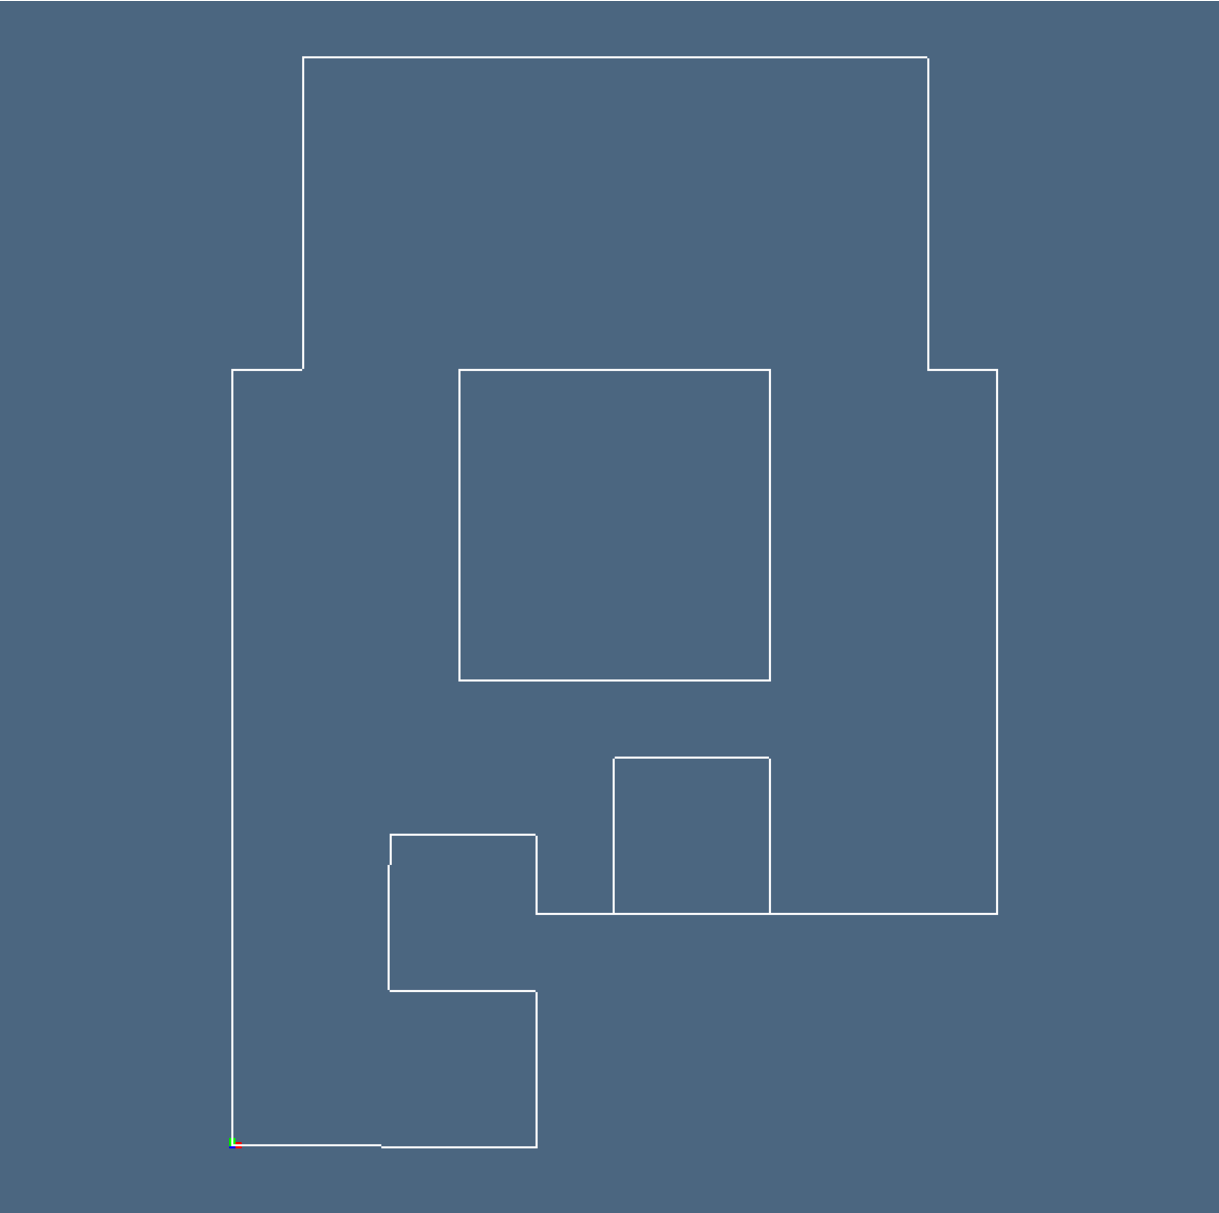
\includegraphics[height=0.243\linewidth,width=0.243\linewidth]{images/frame4} 
   \caption{The 1-complexes and the 2-complex defined by the LAR models by (a) \texttt{(nodes,arcs1)}, (b) \texttt{(nodes,arcs1+arcs2)}, (c) \texttt{(nodes,faces)}, (d) \texttt{(V,[EV[e] for e in boundaryCells(FV,EV)])}, respectively.}
   \label{fig:frames}
\end{figure}

\paragraph{Instancing of structure frame by floor}

Our structural frame, actually a simplified version of \emph{chimera grid} or \emph{overset grid} (see, e.g.~\cite{Meakin:99}) used in Computational Fluid Dynamics, is instanced at the different floors of the hospital model, as shown by the script below.

%-------------------------------------------------------------------------------
@D Instancing of structure frame by floor 
@{""" Instancing of structure frame by floor """
nodes0, arcs10,arcs20, faces0 = structureGrid(mezaninePillars+bottomPillars)
nodes1, arcs11,arcs21, faces1 = structureGrid(mezaninePillars)
nodes2, arcs12,arcs22, faces2 = structureGrid(firstPillars)
nodes3, arcs13,arcs23, faces3 = structureGrid(secondPillars)
nodes4, arcs14,arcs24, faces4 = structureGrid(secondPillars)
nodes5, arcs15,arcs25, faces5 = structureGrid(secondPillars)
nodes6, arcs16,arcs26, faces6 = structureGrid(secondPillars)

V,FV,EV = nodes0,faces0,arcs10

if __name__=="__main__":
    VIEW(STRUCT(MKPOLS((V,EV)) ))
    VIEW(STRUCT(MKPOLS((V,EV + arcs20)) ))
    VIEW(STRUCT(MKPOLS((V,FV)) ))
    VIEW(STRUCT(MKPOLS((V,[EV[e] for e in boundaryCells(FV,EV)]))))
@}
%-------------------------------------------------------------------------------


\paragraph{Assembling the 3D structure frame}
%-------------------------------------------------------------------------------
@D Assembling the 3D structure frame 
@{""" Assembling the 3D structure frame """
if __name__=="__main__":

    Nodes0 = AA(lambda v: list(v)+[4-.3])(nodes0)
    Nodes1 = AA(lambda v: list(v)+[8-.3])(nodes1)
    Nodes2 = AA(lambda v: list(v)+[12-.3])(nodes2)
    Nodes3 = AA(lambda v: list(v)+[16-.3])(nodes3)
    Nodes4 = AA(lambda v: list(v)+[20-.3])(nodes4)
    Nodes5 = AA(lambda v: list(v)+[24-.3])(nodes5)
    Nodes6 = AA(lambda v: list(v)+[28-.3])(nodes6)
    
    Frame0 = STRUCT(MKPOLS((Nodes0, arcs10))+MKPOLS((Nodes1, arcs11))+
        MKPOLS((Nodes2, arcs12))+MKPOLS((Nodes3, arcs13))+
        MKPOLS((Nodes4, arcs14))+MKPOLS((Nodes5, arcs15))+
        MKPOLS((Nodes6, arcs16)) + \
        CONS(AA(T([1,2,3]))(Nodes0+Nodes1+Nodes2+Nodes3+Nodes4+Nodes5+Nodes6))(
        POLYLINE([[0,0,0],[0,0,-4]])  ))
    
    Frame1 = STRUCT(MKPOLS((Nodes0, arcs20))+MKPOLS((Nodes1, arcs21))+
        MKPOLS((Nodes2, arcs22))+MKPOLS((Nodes3, arcs23))+
        MKPOLS((Nodes4, arcs24))+MKPOLS((Nodes5, arcs25))+
        MKPOLS((Nodes6, arcs26)) )
    SteelFrame = OFFSET([.2,.2,.3])(STRUCT([Frame0,Frame1]))
    """
    ConcreteFrame = OFFSET([.4,.4,.8])(Frame0)
    """
    VIEW(Frame0)
    VIEW(STRUCT([Frame0,Frame1]))
@}
%-------------------------------------------------------------------------------


\begin{figure}[htbp] %  figure placement: here, top, bottom, or page
   \centering
   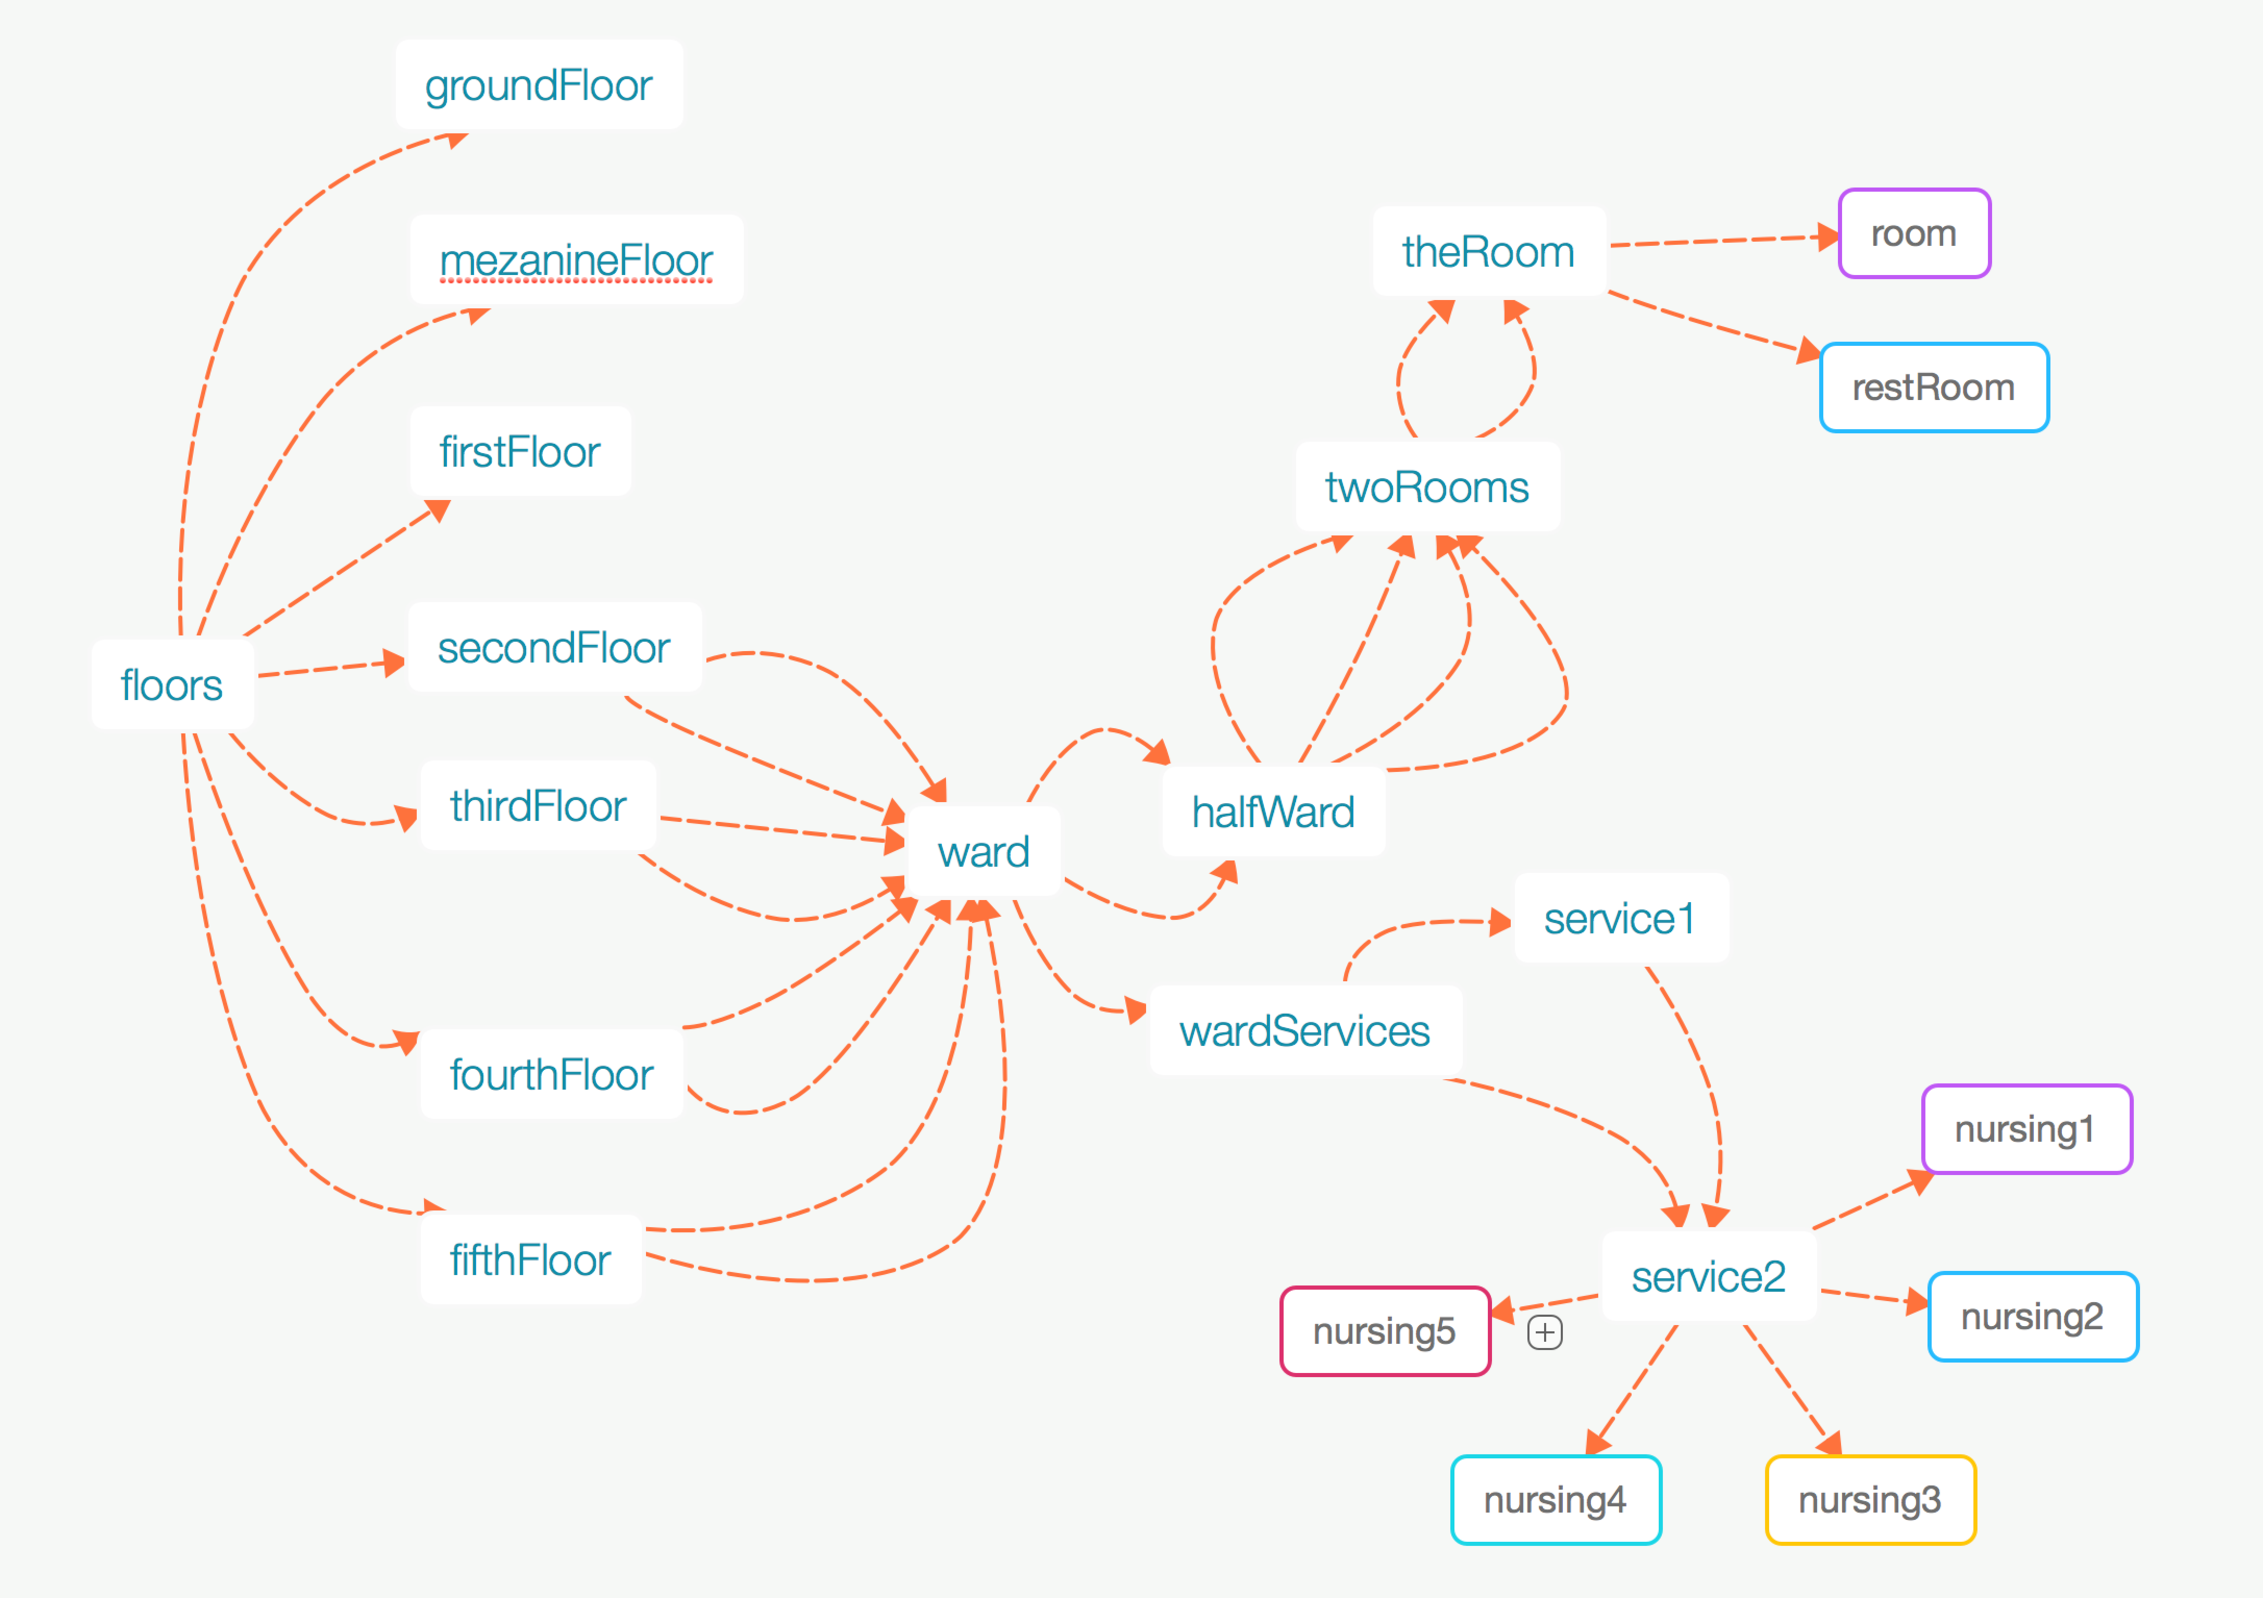
\includegraphics[width=\linewidth]{images/multigraph} 
   \caption{The direct acyclic multigraph representing the hierarchical structure \texttt{floors} of the hospital model. 
   Multiple arcs between a couple of nodes represent the number of different instances of the son node within the father node.}
   \label{fig:multigraph}
\end{figure}

\paragraph{2.5D building assembly}
%-------------------------------------------------------------------------------
@D 2.5D building assembly
@{""" 2.5D building assembly """       
if __name__=="__main__":
 
    floors = Struct([groundFloor,mezanineFloor,firstFloor,
                     secondFloor,thirdFloor,fourthFloor,fifthFloor],"Floors")
    
    floors3D = embedStruct(1)(floors)
    building = Struct(CAT(DISTR([floors3D.body,t(0,0,4)])),"Building")
    V,FV,EV = struct2lar(building,metric)
    VIEW(STRUCT(MKPOLS((V,EV))))
    
    storeys = STRUCT(CAT(DISTR([[ground,mezanine,first,
                    second,third,fourth,fifth],T(3)(4)])))
    VIEW(STRUCT([storeys,SteelFrame] + MKPOLS((V,EV)) ))
@}
%-------------------------------------------------------------------------------


\begin{figure}[htbp] %  figure placement: here, top, bottom, or page
   \centering
   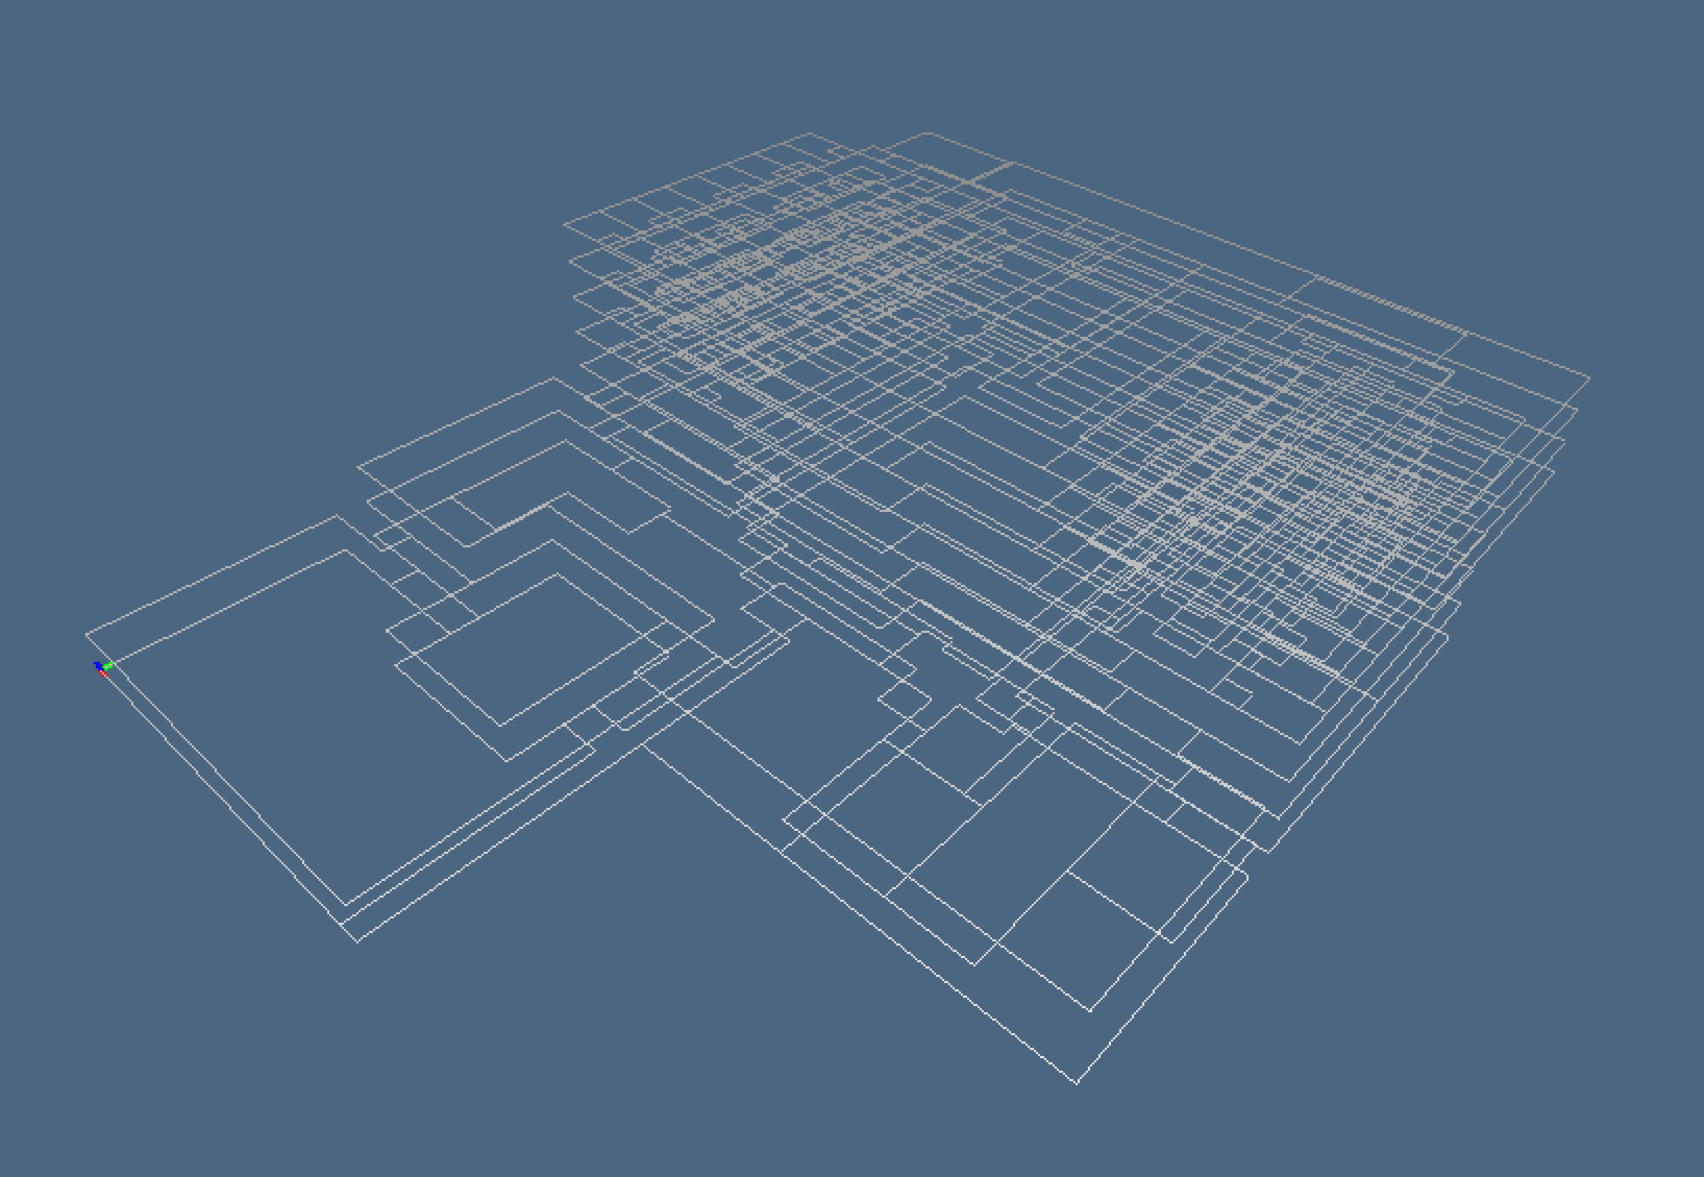
\includegraphics[height=0.35\linewidth,width=0.495\linewidth]{images/floor3D} 
   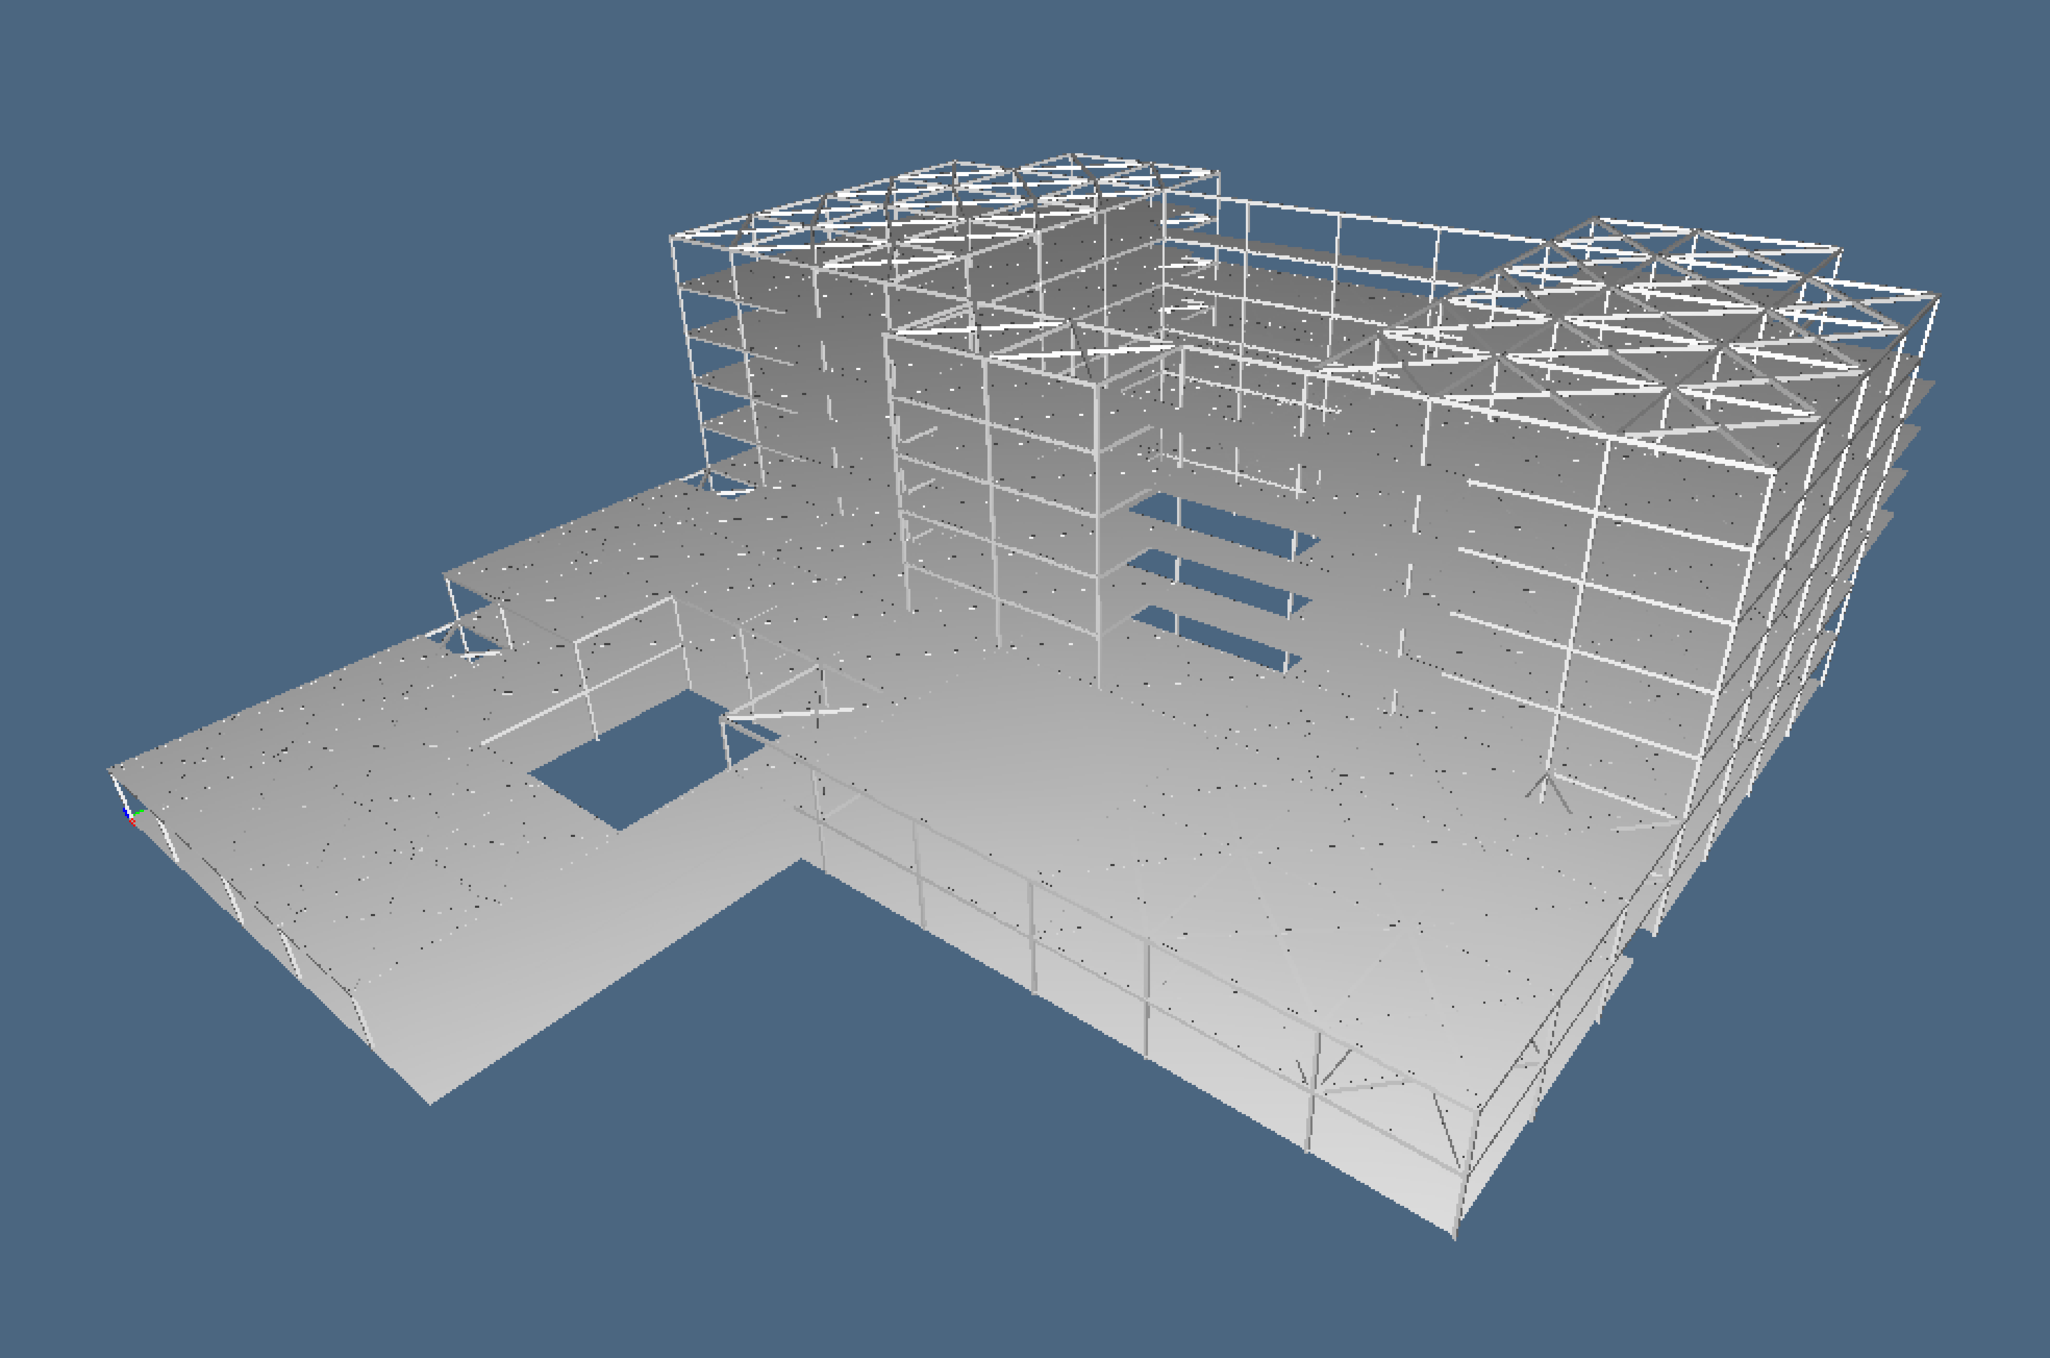
\includegraphics[height=0.35\linewidth,width=0.495\linewidth]{images/floor3Da} 
   \caption{2.5D building assembly: (a) 1-skeletons of 2D floors embedded in 3D; (b) 2-skeletons of floors and 3D structural grid.}
   \label{fig:example}
\end{figure}




\paragraph{2.5D building assembly}
%-------------------------------------------------------------------------------
@D 2.5D building assembly
@{""" 2.5D building assembly """    
"""    
VIEW(STRUCT([ STRUCT(MKPOLS((metric(V),EV))), STRUCT(CONS(AA(T([1,2]))(metric(EXPAND(pillars))))(CIRCLE(.4)([8,1]))) ]))
lars = AA(struct2lar)(floors)
AA(COMP([STRUCT,MKPOLS,CONS([S1,S3])]))(lars)
AA(COLOR)([RED,GREEN,BLUE,CYAN,MAGENTA,YELLOW,BROWN])
colors = AA(COLOR)([RED,GREEN,BLUE,CYAN,MAGENTA,YELLOW,BROWN])
hpcs = AA(COMP([STRUCT,MKPOLS,CONS([S1,S3])]))(lars)
AA(APPLY)(TRANS([colors,hpcs]))
VIEW(STRUCT(AA(APPLY)(TRANS([colors,hpcs]))))
hpcs = AA(COMP([STRUCT,MKPOLS,CONS([COMP([metric,S1]),S3])]))(lars)
VIEW(STRUCT(AA(APPLY)(TRANS([colors,hpcs]))))
pils = STRUCT(CONS(AA(T([1,2]))(metric(EXPAND(pillars))))(CIRCLE(.4)([8,1])))
VIEW(STRUCT(AA(APPLY)(TRANS([colors,hpcs]))+[COLOR(BLACK)(pils)]))
"""
@}
%-------------------------------------------------------------------------------


\begin{figure}[htbp] %  figure placement: here, top, bottom, or page
   \centering
   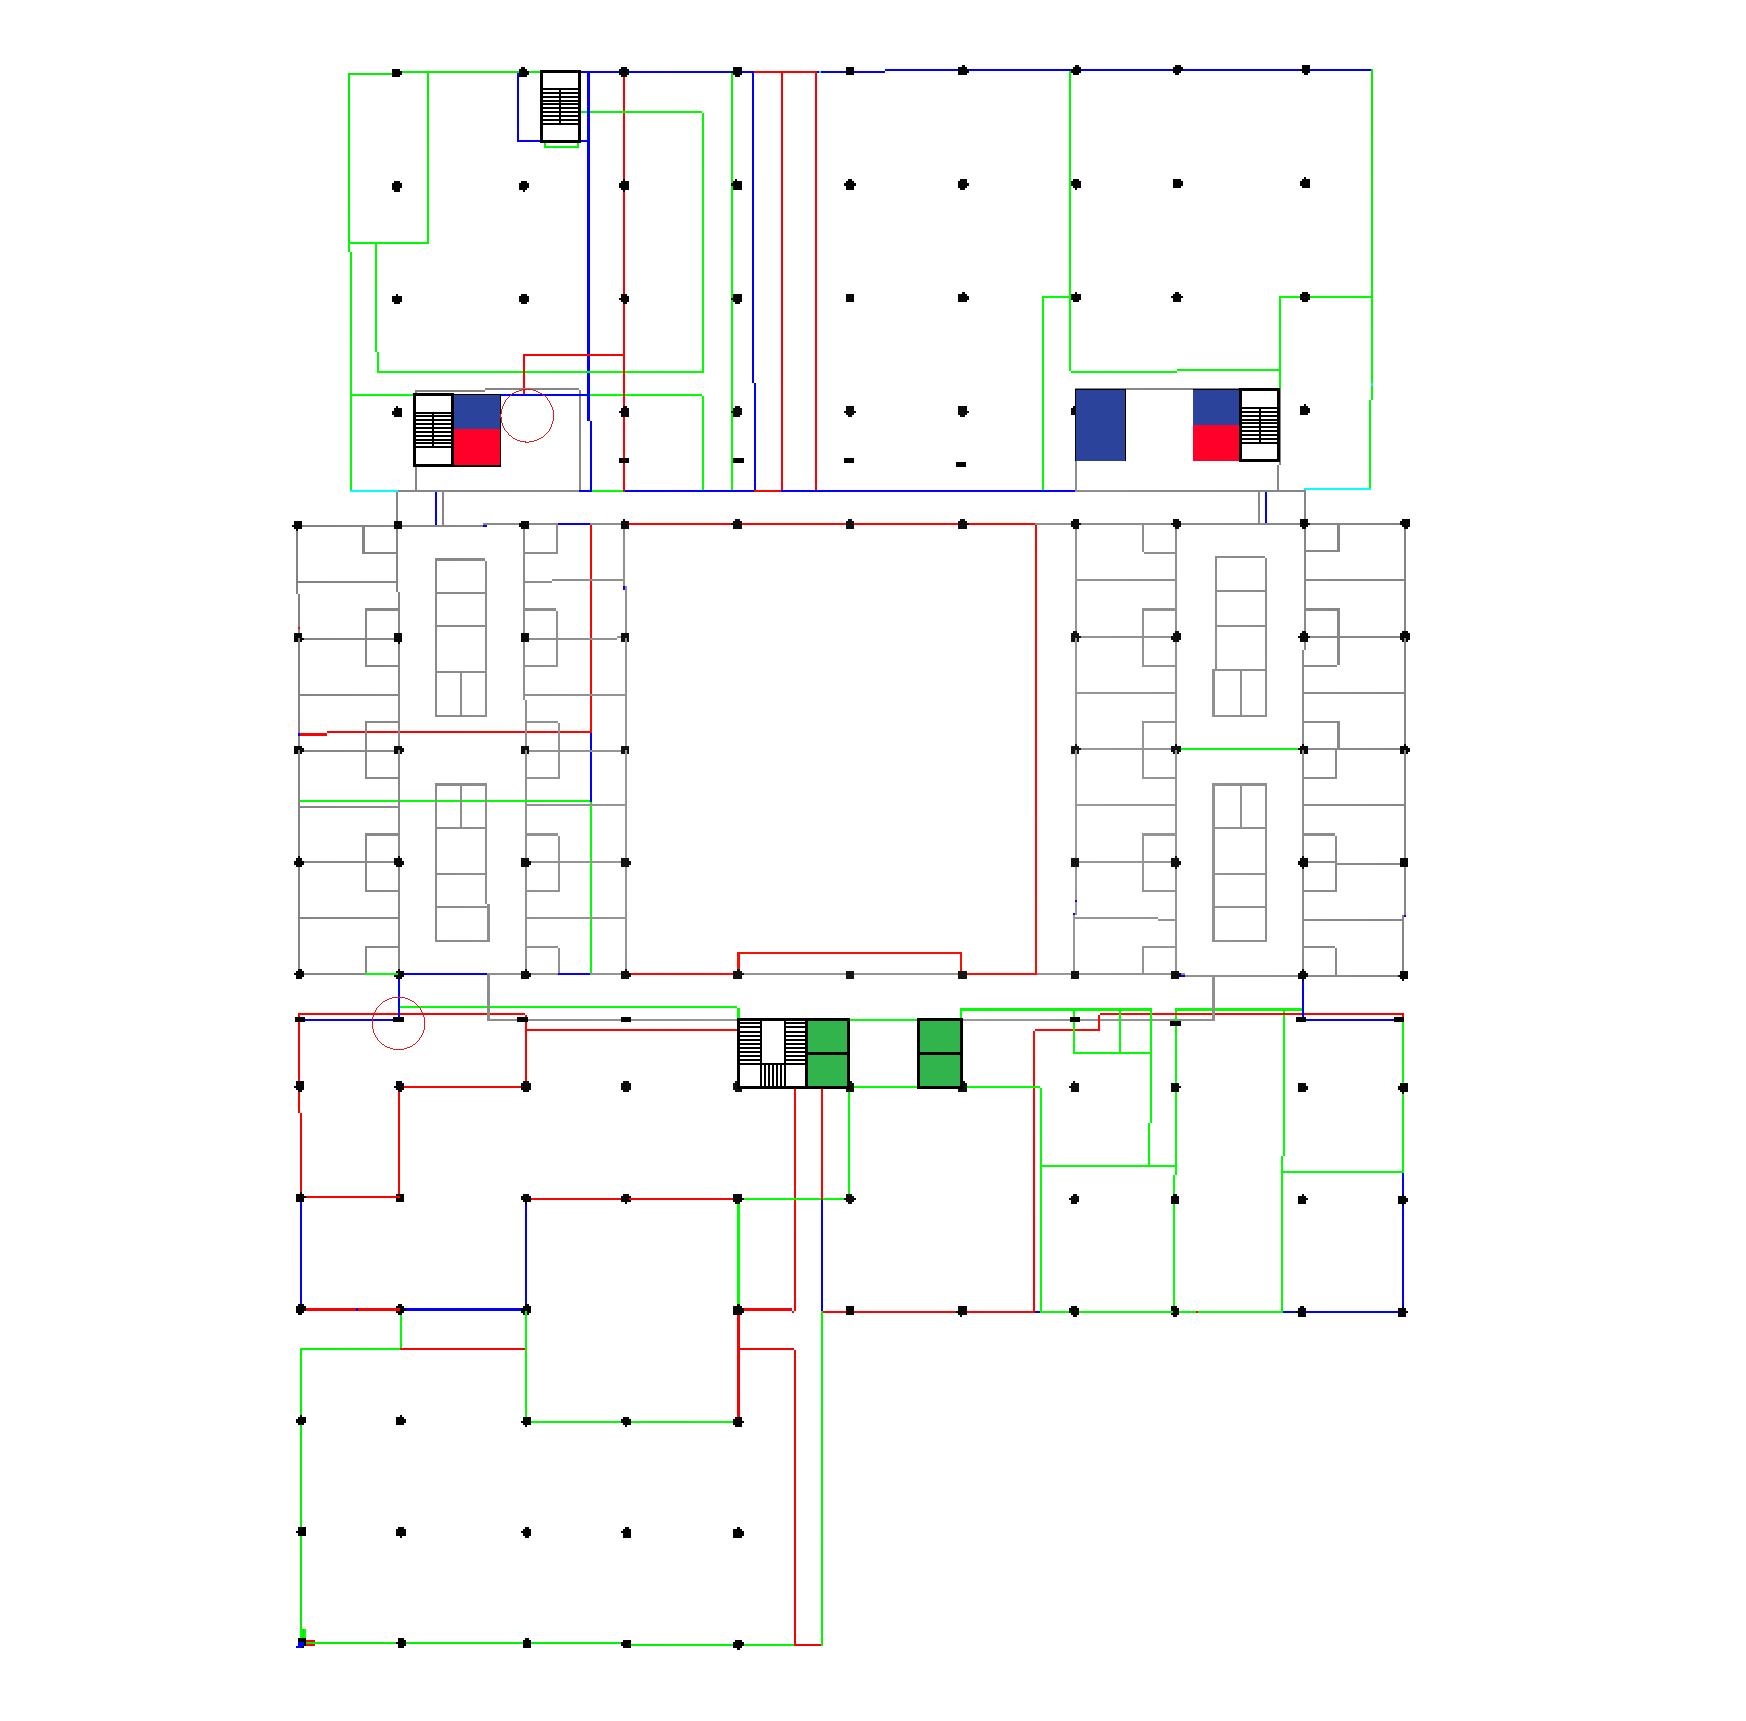
\includegraphics[width=\linewidth]{images/planupdate} 
   \caption{Superimposition of the 2D floors in different colours, and vertical communications of visitors (green); patients (red); personel (blue).}
   \label{fig:example}
\end{figure}


\subsection{Vertical communications}


\paragraph{aaaa}
%-------------------------------------------------------------------------------
@D aaaa
@{""" aaaa """

@}
%-------------------------------------------------------------------------------

%===============================================================================
\section{Design review}
%===============================================================================

The design review is here intended as the computation of the discrete fields of interest,
above the space decomposition generated in the previous design steps. 

As stated in the beginning of this document, the design processing proceeds by step-wise refinement 
of topological (and geometrical) constraints on the planned spaces, aimed to satisfy
a set of design requirements. In case of non-satisfaction, some design changes are introduced, producing a different space decomposition, and repeating the tests.

The discrete field values within the cells of the decomposition provide an evaluated \emph{cochain} over 
a chain (subset of cells) defined above the design decomposition. Both the chain of interest, and the cochain evaluated over it may vary, depending on the design task at hand. In any case the \emph{evaluation} of a cochain $\phi$ above a chain $\rho$, denoted as either $\phi(\rho)$ or the pairing $\langle \phi,\rho \rangle$, will produce a field value, in our case a number, corresponding to the integral of the field (discrete differential form) above the discretized integration domain (set of cells).

%-------------------------------------------------------------------------------
\subsection{Integration and cochains computation}
%-------------------------------------------------------------------------------

Very often, the discrete field value associated to every cell of a cellular decomposition  results from the integration  of some differential $k$-form on the given $k$-cell.  In general, a $k$-form can be described as an entity to be integrated on a $k$-dimensional (sub)region~\cite{Desbrun:2005:DDF:1198555.1198666}.
For this purpose, we are going to  (a)  approximate the given form (function $\R^k \to \R$) with a multivariate polynomial;
(b)    use a finite integration method for $k$-variate monomials in 2D or 3D Euclidean space~\cite{CattaniP-BIL1990}.
The result is a (hierarchical) mapping between the (hierarchy of) cells of the decomposition, and the integral of an approximating polynomial on the cells.

\paragraph{Computing a surface cochain via Struct traversal}

The function \texttt{structCochain}, given in the script below, returns the hierarchical (surface) cochain corresponding to the given \texttt{depth} of the \texttt{struct} input. In particular, every value in the output dictionary \texttt{cochain} returns the evaluated (i.e.~summed) cochain associated to the \texttt{struct} subgraph rooted in every node at  \texttt{depth} distance from the root node of \texttt{struct}. Just notice that the keys of the output \texttt{cochain} dictionary result from the \emph{string-join} of the names of the \texttt{struct} nodes along the \emph{current} path from the root to the node (at level \texttt{depth}) associated with the key.

%-------------------------------------------------------------------------------
@D Computing a surface cochain via Struct traversal
@{""" Computing a surface cochain via Struct traversal """

@< Traversing a hierarchical surface cochain @>

def structCochain(depth=1):
    def structCochain0(struct):
        cochain = defaultdict(int)
        dim = checkStruct(struct.body)
        CTM, stack = scipy.identity(dim+1), []
        cochainMap = structCochainTraversal(CTM, stack, struct, [], [], []) 
        for cell,cochainValue in cochainMap:
            nameArray = cell.split(".")
            cochain[".".join(nameArray[:depth])] += cochainValue[0]
        return cochain
    return structCochain0
    
@< Example of hierarchical surface cochains @>
@}
%-------------------------------------------------------------------------------

\paragraph{Traversing a hierarchical surface cochain}
The \texttt{structCochainTraversal} function given below executes a standard traversal of a hierarchical structure, consisting in relocating all encountered objects from local coordinates to the root coordinates. 

While executing the traversal, a set of pairs (corresponding to each traversed node) is accumulated in the \texttt{cochainMap} list, initially empty. Every such pair contains the joined names of nodes along the current path, and the surface integral evaluated on the traversed node, cast to an integer value. 

Notice that if a \texttt{struct} node contains more than one instance of the same son, then the names of such instances are joined with the counter value associated to the son's \texttt{name} within a dictionary \texttt{repeatedNames}, in order to make individually identifiable the various object instances.

%-------------------------------------------------------------------------------
@D Traversing a hierarchical surface cochain
@{""" Traversing a hierarchical surface cochain """
def structCochainTraversal(CTM, stack, obj, cochainMap=[], names=[], nameStack=[]):
    repeatedNames = defaultdict(int)
    
    def map(model):
        V,FV,EV = larApply(CTM)(model)
        return AA(int)(surfIntegration((metric(V),FV,EV)))
    
    for i in range(len(obj)):
        if isinstance(obj[i],Struct):
            repeatedNames[obj[i].name] += 1
            if repeatedNames[obj[i].name]==1: theName = obj[i].name
            else: theName = obj[i].name + str(repeatedNames[obj[i].name]-1)
            names.append(theName)
            nameStack = nameStack+[names]
            
            stack.append(CTM) 
            structCochainTraversal(CTM, stack, obj[i], cochainMap, names, nameStack)
            CTM = stack.pop()
            theName = names.pop()
            
        elif isinstance(obj[i],Model): 
            cochainMap += [( ".".join(names), map(obj[i]) )]
        elif (isinstance(obj[i],tuple) or isinstance(obj[i],list)) and (
              len(obj[i])==2 or len(obj[i])==3):
            cochainMap += [( ".".join(names), map(obj[i]) )]
        elif isinstance(obj[i],Mat): 
            CTM = scipy.dot(CTM, obj[i])
    return cochainMap
@}
%-------------------------------------------------------------------------------

\paragraph{Example}

Few examples are given below of computation of the surface cochain for the \texttt{ward} and the \texttt{twoRooms} structures, at several different depth depths.

%-------------------------------------------------------------------------------
@D Example of hierarchical surface cochains
@{""" Computing a surface cochain via Struct traversal """
if __name__ == "__main__":
    print "\nsurface cochain(ward) =", structCochain(0)(ward)
    print "\nsurface cochain(ward) =", structCochain(1)(ward)
    print "\nsurface cochain(ward) =", structCochain(2)(ward)
    print "\nsurface cochain(ward) =", structCochain(3)(ward)
    print "\nsurface cochain(ward) =", structCochain(4)(ward)
    print "\nsurface cochain(twoRooms) =", structCochain(1)(twoRooms)
    print "\nsurface cochain(twoRooms) =", structCochain(3)(twoRooms)
@}
%-------------------------------------------------------------------------------


%===============================================================================
\section{System semantics}
%===============================================================================

\subsection{Topological requirements}

\subsection{Geometrical requirements}


%===============================================================================
\section{Code exporting}
%===============================================================================

\paragraph{The \texttt{Hospital.py} module}
%-------------------------------------------------------------------------------
@O larlib/larlib/hospital.py
@{""" The 'Hospital' module """
from larlib import *
from copy import deepcopy
DEBUG = True

@< Reference grid @>
@< Coding utilities @>
@< From array indices to grid coordinates @>
@< Storey input @>
@< Storey generation @>
@< Storey viewing @>
@< Column locations on grid @>
@< Generation of beams and structural chains @>
@< Instancing of structure frame by floor @>
@< Assembling the 3D structure frame @>
@< Structure embedding @>
@< 2.5D building assembly @>
@< Computing a surface cochain via Struct traversal @>
@}
%-------------------------------------------------------------------------------


%===============================================================================
\appendix
\section{Code utilities}
%===============================================================================

\paragraph{Coding utilities}
%-------------------------------------------------------------------------------
@D Coding utilities
@{""" Coding utilities """
@< From grid to metric coordinates @>
@< Mapping a grid frame to a Cartesian one @>
@< Solidify the boundary of polyline-like building units @>
@< Make a struct object from a 2D polyline @>
@}
%-------------------------------------------------------------------------------

\paragraph{Mapping the grid frame to a Cartesian right-hand frame}
%-------------------------------------------------------------------------------
@D Mapping a grid frame to a Cartesian one
@{""" Mapping the grid frame to a Cartesian right-hand frame """
def vmap(YMAX):
    def vmap0(V):
        if len(V[0])==3: W = [[x,YMAX-y,z] for x,y,z in V]
        else: W = [[x,YMAX-y] for x,y in V]
        return W
    return vmap0
                
def embed(z):
    def embed0(p): 
        return p+[z]
    return embed0
@}
%-------------------------------------------------------------------------------

\paragraph{Solidify the boundary of polyline-like building units}
%-------------------------------------------------------------------------------
@D Solidify the boundary of polyline-like building units
@{""" Solidify the boundary of polyline-like building units """
def floor(X,Y):
    def floor0(structure2D,metric=ID):
        V,FV,EV = struct2lar(structure2D,metric)
        BE = [EV[e] for e in boundaryCells(FV,EV)]
        theFloor = SOLIDIFY(STRUCT([POLYLINE([V[v],V[w]]) for v,w in BE]))
        return theFloor,V,EV
    return floor0
@}
%-------------------------------------------------------------------------------

\paragraph{Make a struct object from a 2D polyline}
%-------------------------------------------------------------------------------
@D Make a struct object from a 2D polyline
@{""" Make a struct object from a 2D polyline """
isPolyline = ISSEQOF(ISSEQOF(ISNUM))
isPolylineSet = ISSEQOF(ISSEQOF(ISSEQOF(ISNUM)))

def buildingUnit(polyline,string):
    if ISSEQOF(ISSEQOF(ISNUM))(polyline): model = polyline2lar([polyline])
    else: model = polyline2lar(polyline)
    return Struct([model],str(string))
@}
%-------------------------------------------------------------------------------

\paragraph{Extract 1-cells from the lar of a polylineSet}
%-------------------------------------------------------------------------------
@D Make a struct object from a 2D polyline
@{""" Make a struct object from a 2D polyline """
def lineSet(polylineSet):
    EV = []
    for polyline in polylineSet:
        EV += [(v,w) if v<w else (w,v) for v,w in zip(polyline,polyline[1:]+[polyline[0]])]
    return AA(list)(EV)
@}
%-------------------------------------------------------------------------------
    

\paragraph{The 2.5D mock-up}
%-------------------------------------------------------------------------------
@O test/py/hospital/mock-up.py
@{""" The 2.5D mock-up of an hospital building """

@}
%-------------------------------------------------------------------------------


\bibliographystyle{amsalpha}
\bibliography{hospital}

\end{document}
